%%---------------------
%% THESIS - REPORT -DRAFT
%% AMAREN PRASANNA DAS
%% REPORT COMPLETED ON: 
%% THESIS DATE: 
%%---------------------
%\documentclass[a4paper, 12pt]{report}
\documentclass[a4paper, 12pt, notitlepage]{report}
%%%%%%%%%%%%%%%%%%%%%%%%%%%%%%%%%%%%%%%%%%%%%%%%%%%%%%%%%%%%%%%
\usepackage{graphicx}
\usepackage{setspace}%for double spacing etc
\usepackage[top=1.0in, bottom=1.0in, left=1.5in, right=1.0in, twoside]{geometry}
\usepackage{emptypage}%to make empty pages number less and to use \cleardoublepage
\usepackage{longtable}%for long table in nomenclature
%\usepackage[none]{hyphenat}%to remove hyphenation
\usepackage{adjmulticol}%for multiple columns in certificate
%\usepackage{tikz}%for flow charts
%\usetikzlibrary{shapes,arrows,positioning}
%\usepackage{algorithm} 
%\usepackage{algorithmicx}
%\usepackage{algpseudocode}
%\usepackage{cite}%for combining citations when referred together
%\usepackage{natbib}
%\usepackage[comma,authoryear]{natbib}
\usepackage{epstopdf} 
\usepackage{blindtext}
%\hyphenpenalty=10000
\usepackage{caption}
\usepackage{subfigure}
\usepackage{latexsym}
\usepackage{float}
\usepackage{textcomp}
\usepackage{gensymb}
\usepackage{upgreek}
\usepackage{lmodern}
\usepackage{textcomp}
\usepackage{url}
\usepackage[T1]{fontenc}
%\usepackage{isomath} 
\usepackage{bm}
\usepackage{lipsum}
\usepackage{enumerate}
\usepackage{amsmath}
\usepackage{ amssymb}
%\usepackage{subcaption}
 % % ADDITIONAL TO COMMENT IN FINA
%\usepackage{slashbox} % For two title in a box
\usepackage{hyperref}
\usepackage{color}
\usepackage{algorithm}
\usepackage{algpseudocode}
\usepackage{rotating} % For sideways table
\usepackage{adjustbox}
\usepackage{booktabs}
\usepackage{color}
\usepackage{multirow}
\usepackage{xcolor,colortbl} % Colored Row in Table

\providecommand{\greektext}{\fontencoding{LGR}\selectfont\def\encodingdefault{LGR}} 
\providecommand{\textgreek}[1]{\leavevmode{\greektext #1}} 
%%%%%%%% For Integration in Sobol Method %%%%%%%%%%%%%%%%%%%%%%%%%%%%%%
\DeclareMathOperator*{\uint}{\scalerel*{\rotatebox{8}{$\!\scriptstyle\int\!$}}{\int}}
\usepackage{scalerel}
%%%%%%%%%%%%%%%%%%%%%%%%%%%%%%%%%%%%%%%%%%%%%%%%%%%%%%%%%%%%%%%%%%%
\def\mathbi#1{\textbf{\em #1}} 
%%%%%%%%%%%%%%%%%%%%%%%%%%%%%%%%%%%%%%%%%%%%%%%%%%%%%%%%%%%%%%%%%%%
\usepackage{tikz}
\newcommand*\circled[1]{\tikz[baseline=(char.base)]{
        \node[shape=circle,draw,inner sep=1pt] (char) {#1};}}
\newcommand{\algrule}[1][.2pt]{\par\vskip.5\baselineskip\hrule height #1\par\vskip.5\baselineskip}
\renewcommand{\thealgorithm}{\arabic{chapter}.\arabic{algorithm}} 
\DeclareMathAlphabet\mathbfcal{OMS}{cmsy}{b}{n}
%%%%%%%%%%%%%%%%%%%%%%%%%%%%%%%%%%%%%%%%%%%%%%%%%%%%%%%%%%%%%%%%%%%
\usepackage{pseudocode}
%%%%%%%%%%%%%%%%%%FOR Appendix%%%%%%%%%%%%%%%%%%%%%%%%%%%%%%%%%%%%%%%%

%%%%%%%%%%%%%%%%%%%%%%%%%%%%%%%%%%%%%%%%%%%%%%%%%%%%%%%%%%%%
\usepackage{geometry}
\usepackage{afterpage}

\usepackage{hyphenat}

%%%%%%%

\setcounter{tocdepth}{4}
\setcounter{secnumdepth}{4}


\begin{document}
\pagenumbering{roman}
\newgeometry{top=1.3in,bottom=1.0in,left=0.8in,right=0.8in}
\doublespacing
\thispagestyle{empty}
\begin{center}



\textbf{\large{DESIGN AND CONTROL OF TELE OPERATED MOBILE PLATFORM}}

\bigskip
\bigskip
\bigskip
\bigskip
\bigskip
\bigskip
\bigskip
\bigskip
\bigskip
\bigskip

\textbf{AMAREN PRASANNA DAS}

\bigskip
\bigskip
\bigskip
\bigskip
\bigskip
\bigskip
\bigskip
\bigskip
\bigskip
\bigskip
\bigskip
\bigskip
\bigskip
\bigskip
\bigskip
\bigskip
\bigskip
\bigskip
\bigskip
\bigskip
\bigskip


\includegraphics[height=4cm]{Misc_front/iitlogo.eps}

\bigskip
\bigskip
\bigskip
\bigskip
\bigskip
\bigskip

\textbf{DEPARTMENT OF MECHANICAL ENGINEERING}

\textbf{INDIAN INSTITUTE OF TECHNOLOGY DELHI}

\textbf{OCTOBER 2018}



\end{center}
%%%%%%%%%%%%%%%%%%%%%%%%%%%%%%%%%%%%%%%%%%%%%%%%%%%%%%%%%%%%%%%%%%%%%%%%
\newpage
\thispagestyle{empty}
\vspace*{\fill}
\textbf{ \textcopyright Indian Institute of Technology Delhi (IITD), New Delhi, 2017}
\vspace*{\fill}
\mbox{}
%%%%%%%%%%%%%%%%%%%%%%%%%%%%%%%%%%%%%%%%%%%%%%%%%%%%%%%%%%%%%%%%%%

\newpage
\thispagestyle{empty}
\begin{center}



\textbf{\large{DESIGN AND CONTROL OF TELE OPERATED MOBILE PLATFORM}}

\bigskip
\bigskip
\bigskip
\bigskip
\bigskip
\bigskip
\textbf{by}
\bigskip
\bigskip

\textbf{AMAREN P DAS}

\bigskip
\bigskip

\textbf{Department of Mechanical Engineering}

\bigskip
\bigskip
\bigskip
\bigskip
\bigskip
\bigskip


\textit{Submitted}

\textit{in fulfillment of the requirements of the degree of Doctor of Philosophy}

\bigskip
\bigskip

\textbf{}

\bigskip
\bigskip

\textit{to the}

\bigskip
\bigskip
\bigskip
\bigskip
\bigskip
\bigskip
\bigskip


\includegraphics[height=4cm]{Misc_front/iitlogo.eps}

\bigskip
\bigskip



\textbf{INDIAN INSTITUTE OF TECHNOLOGY DELHI}

%\textbf{HAUZ KHAS, NEW DELHI - 110016}

\textbf{OCTOBER 2018}
\end{center}
%%%%%%%%%%%%%%%%%%%%%%%%%%%%%%%%%%%%%%%%%%%%%%%%%%%%%%%%%%%%%%%%%%%%%%%%
\mbox{}
%%%%%%%%%%%%%%%%%%%%%%%%%%%%%%%%%%%%%%%%%%%%%%%%%%%%%%%%%%%%%%%%%%
\restoregeometry
\newgeometry{top=1.3in,bottom=1.0in,left=1.2in,right=0.8in}
\doublespacing
%%%%%%%%%%%%%%%%%%%%%%%%%%%%%%%%%%%%%%%%%%%%%%%%%%%%%%%%%%%%%%%%%%%%%%%%
\pagenumbering{roman}
\newpage
\thispagestyle{empty}
\mbox{}
%%%%%%%%%%%%%%%%%%%%%%%%%%%%%%%%%%%%%%%%%%%%%%%%%%%%%%%%%%%%%%%%%%
\newpage
\thispagestyle{empty}
\begin{center}
\textbf{\Large{Certificate}}
\end{center}

\addcontentsline{toc}{section}{Certificate}
This is to certify that the thesis entitled \textbf{DESIGN AND CONTROL OF TELE OPERATED MOBILE PLATFORM}, submitted by   \textbf{Shri. Amaren Prasanna Das} to the Indian Institute of Technology Delhi, for the award of the degree of \textbf{Doctor of Philosophy} in Mechanical Engineering, is a record of the original, bona-fide research work carried out by him under my supervision and guidance. The thesis has reached the standards fulfilling the requirements of the regulations related to the award of the degree.

The results contained in this thesis have not been submitted in part or in full to any other university or institute for the award of any degree or diploma.
\bigskip
\bigskip
\bigskip
\bigskip
\bigskip


\textbf{Dr. S. K. Saha}

Professor

Department of Mechanical Engineering

Indian Institute of Technology Delhi

New Delhi - 110016, India





%%%%%%%%%%%%%%%%%%%%%%%%%%%%%%%%%%%%%%%%%%%%%%%%%%%%%%%%%%%%%%%%%%%%%%%%

\restoregeometry
\newgeometry{top=1.3in,bottom=1.0in,left=1.5in,right=1.0in}
\doublespacing
%%%%%%%%%%%%%%%%%%%%%%%%%%%%%%%%%%%%%%%%%%%%%%%%%%%%%%%%%%%%%%%%%%%%%%%%
%\pagenumbering{roman}
\newpage
\thispagestyle{empty}
\mbox{}
%%%%%%%%%%%%%%%%%%%%%%%%%%%%%%%%%%%%%%%%%%%%%%%%%%%%%%%%%%%%%%%%%%

\newpage
%\thispagestyle{empty}

\begin{center}
\textbf{\Large{Acknowledgements}}
\addcontentsline{toc}{section}{Acknowledgements}
\bigskip
\bigskip
\end{center}

The work presented in this thesis would not have been possible without the assistance
of countless individuals.  I extend my eternal gratitude  to all those people. However, despite being a dangerous practice, I would like to single out a few, select, individuals for special recognition.

 This thesis would not have seen the light of the day without the continuous and persistent motivation of my guide Prof. S. K. Saha. His advice and guidance  on technical  issues helped give direction to this research. Moreover, he played a pivotal role in providing the much needed psychological and emotional support. Each and every meeting with him was a booster to my self confidence. 
 
    
I am deeply grateful to my co-supervisor, Professor S. Bhasin in the Department of Electric Engineering at  IIT-Delhi, for his continued encouragement and invaluable suggestions in the field of control engineering and in particular adaptive control during this work. He has been instrumental in introducing me to the latest research results  in the field of time delayed non-linear systems.  
I also express my gratitude to Dr. Deepak N Badodkar, my supervisor at my parent organization BARC, Mumbai for his encouragement and the logistic support he had provided throughout the tenure of my research. Without his support the development and fabrication  of the  physical system would not have been possible.  


It will be imprudent not to mention the help and support provided by my colleague Shri. Rahul V Sakrikar. One person, on whom I fell back in case of any hardware issues be it electrical or mechanical. While discussing and sorting out technical glitches I found his profound experience and field knowledge highly enriching. I still remember his \textit{encouragin}g words, ``Are tera PhD ka kya hua? Saha kuch kaam nahi deya kya?" Another colleague, Shri Shishir Kr. Singh has provided his selfless service to help me develop all the software required for running the actual system. Without his help and support it would have been impossible to conduct experimental runs and data collection. I express my deepest regards to both of them.

I cannot forget the support and help of my co-researchers and classmates Dr. Riby Abraham, Dr. Parmanand Nandihal, Dr. Abdullah Aamir Hayat and Dr. Arun Dayal Uday during my stay and course work at IIT-Delhi. Thereafter, providing all kinds of logistic support at IIT-Delhi. Without their help it would have been impossible to continue my work at IIT-Delhi. I thank them from the bottom of my heart and wish them grand success  in their life.


Finally, I thank my two daughters, Akaisha and Sayuri, my mother for their patience  and support. Special thanks to my wife Namrata, who had taken upon herself  the responsibility of managing the family during my course work at IIT-Delhi and providing the required time and space for my research work thereafter. In absence of  her support, patience and companionship this journey would not have been completed.  



\bigskip
\bigskip
\bigskip
\bigskip

\hfill \textbf{Amaren Pasanna Das}

%%%%%%%%%%%%%%%%%%%%%%%%%%%%%%%%%%%%%%%%%%%%%%%%%%%%%%%%%%%%%%%%%%%%%%%%
\restoregeometry

\doublespacing
\addcontentsline{toc}{section}{Abstract}
%%\section*{Abstract}
\begin{abstract}
\noindent 
 A customized mobile manipulator was designed, developed and fabricated  for radiation measurement and mapping. The detail design aspects based on the environment and mission requirement is presented in the thesis. The dynamic model of the system was developed and simulations were performed for specific paths to verify the actuator requirements and response time. The user interface and control architecture implemented on the mobile robot for teleoperation  were developed for convenient and reliable function of the same. The time delay introduced due to  video data transfer and its effects on system's stability and poor operator performance is demonstrated using simulations. A predictive display of the remote environment based on mathematical model of the mobile robot  and RGB-Depth sensor data received from remote location was proposed, which was practically implemented. This strategy has largely improved robot's navigation by the operator even over significantly  delayed communication network. 

%\lipsum[3-5]

\end{abstract}

%%%%%%%%%%%%%%%%%%%%%%%%%%%%%%%%%%%%%%%%%%%%%%%%%%
%\section*{Abstract}
\begin{abstract}
\noindent 
 A customized mobile manipulator was designed, developed and fabricated  for radiation measurement and mapping. The detail design aspects based on the environment and mission requirement is presented in the thesis. The dynamic model of the system was developed and simulations were performed for specific paths to verify the actuator requirements and response time. The user interface and control architecture implemented on the mobile robot for teleoperation  were developed for convenient and reliable function of the same. The time delay introduced due to  video data transfer and its effects on system's stability and poor operator performance is demonstrated using simulations. A predictive display of the remote environment based on mathematical model of the mobile robot  and RGB-Depth sensor data received from remote location was proposed, which was practically implemented. This strategy has largely improved robot's navigation by the operator even over significantly  delayed communication network. 

%\lipsum[3-5]

\end{abstract}


%%%%%%%%%%%%%%%%%%%%%%%%%%%%%%%%%%%%%%%%%%%%%%%%%%

\cleardoublepage
\tableofcontents
\addcontentsline{toc}{section}{\listfigurename}

\cleardoublepage
\listoffigures

\cleardoublepage
\addcontentsline{toc}{section}{\listtablename}
\listoftables

\cleardoublepage
\addcontentsline{toc}{section}{Important Symbols and Abbreviations}
\include{Misc_front/nomenclature}

\cleardoublepage
\doublespacing
\pagenumbering{arabic}


\chapter{{Introduction}}
\label{ch_1}
The use of robots such as robotic arm  has been used in factories for a long time, basically for repetitive kind  of job. Though it started with the intention to reduce human labour, production cost and increased productivity. With development of technology ,  their scope has expanded beyond  manufacturing domain. Robots are now being used for health care, surveillance, exploration etc. The reduction in development cost of  robotic system has resulted in introduction of robotic system in entertainment industries and personal care. Robots have matured form heavy duty serial linked mechanical arms to a more presentable form such as ASIMO by Haonda and Aibo by Sony.  

 In areas where human access is not preferred or restricted  due to risk of life or inhospitable environmental conditions such as which exists in chemical, space or nuclear industries, robotic systems have gained huge popularity in providing services as surveillance, rescue, exploration \& remote maintenance.  Research in teleoperated and autonomous mobile robotics has been fuelled largely by these  requirement. Teleoperated mobile robots are suitable for these applications  as the work space required to be covered is very large and it is essential to maintain  physical separation between the robot and its control station,   moreover the remote environment is in general unknown. 
 
 This research too was motivated by a similar requirement for in-situ measurement of the radioactive radiation, mostly neutron field, inside the vault and cave areas of   K-130,  K-500  and Medical Cyclotron operational at VECC, Kolkata, West Bengal. Cyclotrons are used to accelerate  charged particle beam to high energy. These are required for experiments in nuclear physics and nuclear medicine. The particles are accelerated to high energy using a high frequency alternating voltage which is applied between two hollow "D"-shaped sheet metal electrodes called "Dees" inside a vacuum chamber. The area surrounding the Dee is called the vault  and cave is the areas where beam line (beam of  accelerated particles) is available for experimentation. Radiation mapping of these areas are  mandatory requirements for getting safety clearance from regulators during  commissioning of new units and at regular intervals during operational life of the cyclotron facility.   Though there are radiation detectors placed at different locations in these area they can only measure radiation levels at discrete location but can not provide the 3-D radiation  map. The advantage of having a  radiation map is that it  provide detailed  input to health physicist  of the dose a person may receive and accordingly plan emergency  operations. These maps also provide the plant operators with the location of radiation leakage and accordingly tune there system to improve its efficiency.

The challenge faced for in-situ inspection during operation of cyclotron is that the interaction  between  an  accelerated  beam   of  charged  particles  and  the  target  produce Bremsstraghlung and characteristic x-rays, prompt $\gamma$-rays, neutrons and delayed radiation ($\beta $ and $\gamma$) thus making human presence unacceptable.  A teleoperated mobile robot with wireless communication link is the obvious solution. This thesis discusses design analysis and develop of a prototype robot  to carry out in-situ measurement and mapping of radiation level.

\section{Research Contributions}
The original contributions of the present research are listed below:
\begin{enumerate}[(i)]

\item Design of customized teleoperated mobile robot for remote surveillance and mapping application.
\item Development of kinematic and dynamic model of the robot at hand.
\item Control architecture required for intuitive teleoperation of this mobile robot.
\item Predictive visual feedback control to alleviate problem arising due to time delayed.


\end{enumerate}
\section{Thesis Organization}
The thesis contains eight chapters and one appendix. They are organized as follows:
\paragraph*{Chapter 1: Introduction\\}
The present chapter, discusses the scope of mobile robotics in general and the motivation which lead to this research followed by the organization of the thesis.
\paragraph*{Chapter 2: Literature Review\\}
This chapter presents the literature review in the following areas \textit{kinamatics and dynamics} of mobile robot, \textit{control of mobile robot}, \textit{control for time delay systems}, \textit{performance of operator under teleopreration}  and \textit{predictive display systems}.

\paragraph*{Chapter 3: Design of Mobile Platform\\}
This chapter highlights the design considerations of tele-operated mobile platform based on environmental conditions mission requirements. This paper presents the design and control scheme of a mobile manipulator used for radiation survey of Cyclotron vault and cave regions. It discusses the mechanical design for the traction system, the steering gear and the scissor mechanism. Selection of  steering system based on terrain condition and power requirement is also discussed.   
\paragraph*{Chapter 4: Mathematica Modelling of Wheeled Mobile Platform \\}
In this chapter, we present the orthogonal compliment method for deriving the dynamic equation of four wheeled differentially driven platform. The platform has two actuated wheels and two passive wheels. Different types of passive wheels has been studied and there corresponding dynamic equation are presented. The main contribution of this paper is derivation of dynamic equation a differentially driven  mobile platform with the most general form of passive wheel.
\paragraph*{Chapter 5:Control of mobile manipulator \\}
The control architecture and the hardware used for tele-operation is presented along with the detailed description of implementation of the controller software at both the remote (mobile robot)  and the local station. The experimental results of robots position based on wheel odometry and is torque requirement for few predefined paths is presented. A comparison study  with the simulated results based on dynamic analysis presented in chapter 4 is also presented.  
\paragraph*{Chapter 6: Simulation Time Delay Tele-operation \\}

In this chapter simulation of a teleoperated mobile platform is presented both under time delay due to communication link and without time delay. It is shown via simulation that with increase in time delay the stability of the teleoperation loop become unstable. A mathematical model of human driver is also presented to simulate the human factor in the teleoperation loop.
 
\paragraph*{Chapter 7: Predictive Display \\}
In this chapter we propose a Predictive Display strategy to counter the time delay in video feedback by extrapolating in time  the camera view based on the predicted position of the robot at remote location. 

\paragraph*{Chapter 8: Conclusions\\}
This chapter summarizes major results of this research work. Limitations along with the future scope from the present experiences are also addressed.


\paragraph*{Bibliography}
\paragraph*{Appendix A:  Measurement of Time Delay in Video Feedback  \\}
Here the experimental set up and methodology used to determine the time delay is presented.
%\paragraph*{Appendix B:  Dynamics  \\}
In this appendix, 


\cleardoublepage
\setcounter{secnumdepth}{4} 
\chapter{Literature Review}
\label{c2_LitRev}

In this chapter, we  discuss some of the important works published pertaining to the scope of this thesis. Few of the techniques and methods published in these literatures are directly used. The section on \textit{Special Purpose Robots} lists literature which were reviewed to arrive at the overall design of the mobile robot developed in this research.
 The dynamic analysis of the mobile platform was based on the works cited in section\textit{ Mathamatical Modeling}. 
 The literature discussed in \textit{Path Tacking } helped to arrive at the "human model" proposed in this thesis for simulation of teleoperation. 
 The section on \textit{Tele-operation} discusses literature in a much broader sense; such as force feedback, haptic interface  design, etc., than what was adapted in this thesis. 
 This was done for completeness of the subject. 
 Last section on \textit{Predictive Display}, though a part of human interface for tele-operation is discussed separately because it forms one of the major components of the tele-operation system network designed  for the mobile robot  presented in this thesis.   
\section{ Special Purpose Robots}
This section reviews some of the special purpose  robots built for various typical applications. 
Design and fabrication of a low cost, solar powered mobile robot for  scientific missions on the Antarctic plateau was presented by Ray  \cite{ray2005design}. Honeycomb-glass-fibre composite was used to provide high strength and low weight. Ohno, et al. \cite{ohno2011robotic}   developed a robotic  vehicle shown in Figure \ref{fig:fukuRobot} for measuring the radiation in the Fukushima Daiichi Nuclear Power Plant. A survey of different types of climbing robots for non-destructive testing of pressure vessel is given by \cite{luk2006tele}, such as NERO III shown in Figure \ref{fig:nero3}.  Briones \cite{briones1994wall} presents a vacuum cup based wall climbing robot for inspection of  nuclear power plants. Galt \cite{galt1997tele} has developed eight-legged teleoperated mobile robot for the use in nuclear industry. Development of a magnetic-wheel based mobile robot for painting of ship is discussed by Cho \cite{cho2013study}. Compliant link based mobile robot was designed and tested by Borenstein\cite{borenstein1995control}, in which the author claims that due to its unique design, better dead-reckoning accuracy was achieved compared to other contemporary designs. This vehicle has two independent drive units or "trucks" that are free to rotate about a vertical shaft connected to the vehicle body. Each truck comprises two drive motors on a common axes and forms a differential drive system. Mechanical compliance was implemented by means of a linear bearing that allows relative motion between the front and rear truck. Other literature giving details of  mobile robots based on   differential wheel, traction belt and omnidirectional wheel are given in the introductory part of Chapter \ref{ch_3:Design}.
 \begin{figure}
	\centering
	\begin{minipage}{.5\textwidth}
		\centering
		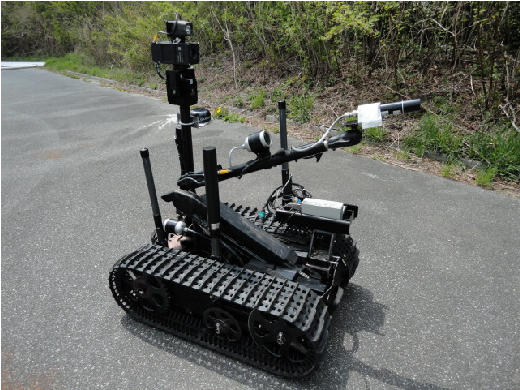
\includegraphics[height=5cm,keepaspectratio]{Chapter2/fig/FukusimaRobot}
		\captionof{figure}{Robot for Fukushima Daiichi \\  Source:  Ohno, et al  \cite{ohno2011robotic} }
		\label{fig:fukuRobot}
	\end{minipage}%
	\begin{minipage}{.5\textwidth}
		\centering
		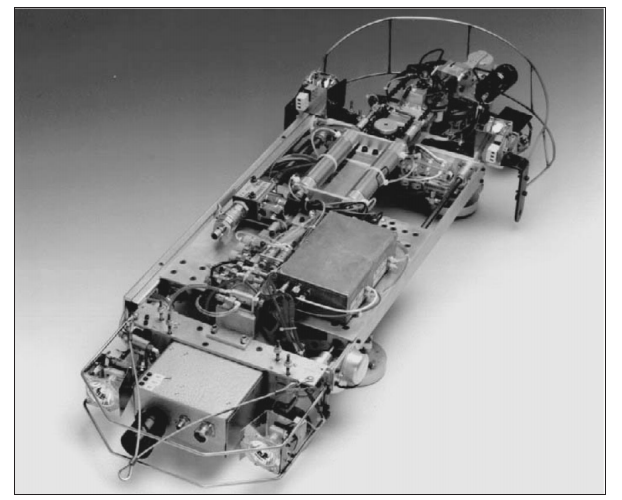
\includegraphics[width=1\linewidth,height=5cm,keepaspectratio]{Chapter2/fig/nero3}
		\captionof{figure}{NERO III \\ Source: Luk et al \cite{luk2006tele}}
		\label{fig:nero3}
	\end{minipage}
\end{figure}

   
\section{Mathematical Modeling}
A very comprehensive list of Wheeled Mobile Robots (WMR) using different wheel configuration is given by Muir and Neuman \cite{muir1987kinematic}. In the paper, kinematic equations of conventional, omnidirectional and ball wheels were presented. The kinematics of the WMR was derived by combining the kinematic information of   individual wheel. Detection of wheel slip based on  error in the least square solution was also discussed. Similar issues were addressed by Alexander in \cite{alexander1989kinematics}. The major difference is that he uses physical friction model in the analysis of over actuated systems where rolling constrains are not satisfied. A seminal work by Champion \cite{campion1996structural} gives the structural classification of wheeled mobile robots based on the \textit{degree of mobility}, $\delta_m$, and \textit{degree of steeribility}, $\delta_s$. It was based on the number of conventional fixed wheels and  conventional centered orientable wheels. According to them any WMR fall in one of the 5 categories given by $(\delta_m,\delta_s)\rightarrow(3,0),(2,1),(1,1),(1,2)$. 
The configuration and posture kinematic models of each type was derived. Based on  dynamic model, the minimal number of actuators required for full maneuverability of each type was presented. Kinematic analysis of omi-directional over-actuated mobile robot  was presented in \cite{yi2002kinematics}. Two different methods for forward kinematics was also discussed along with  singularity analysis. Actuator switching scheme based on load distribution to avoid singularity was also presented. 

Dynamic modeling of mobile manipulator can be categorized as: force based ,i.e, the Newtaon-Eular (NE) formulation and  energy based as in Eular-Lagrange (EL) equations. Hoostmans \cite{hootsmans1992motion} used NE method to arrive at  the dynamic model of a mobile manipulator that has two links mounted on a mobile platform. Chung \cite{chung1998interaction} used EL method to arrive at the equations of motion for a mobile manipulator. Geometric mechanics was used to adapt Luh and walker \cite{luh1980line} algorithm  by Boyer and Ali \cite{boyer2011recursive} to apply recursive inverse dynamics formulation to wheeled systems.   

Orthogonal compliment method utilizes the advantage of NE and EL approach to derive the equations of motion of  a multibody  system.  It uses the fact that the motion can take place only in the null space of the constrains inducing matrix $A$ defined as $Ax=0$, where $x$ is a vector of independent co-ordinates. The orthogonal compliment of the constraint inducing matrix $A$ is used to eliminate the non-working constraint  forces  and moments from the equations of motion.  Angeles and Lee \cite{angeles1988formulation} used the natural orthogonal compliment method to derive the equations of motion for holonomic mechanical systems. In this,  orthogonal compliment was derived from the velocity constraints naturally, hence the name. This was  used by Angeles \cite{angeles2013fundamentals} and Saha in \cite{saha1989kinematics},\cite{saha1991dynamics} to derive the equations of motion for a WMR. 

\section{Path Tracking}
Path tracing algorithm for the control of a mobile robot is used to arrive at the mathematical model of a human operator for simulation of tele-operation loop, as done in chapter 6. Geometry based path tracking algorithms are most intuitive and hence suitable for the present application. The major algorithms in this  category reported in the literatures are \textit{pure pursuit} \cite{coulter1992implementation}, \textit{follow the carrot} \cite{barton2001controller}, \textit{vector pursuit} \cite{wit2004autonomous}, and \textit{follow the past} \cite{hellstrom2006follow}. In pure-pursuit \cite{coulter1992implementation}, the steer angle of the robot is set so that the robot moves in circle to reach a \textit{ goal point} on the desired path. The goal point is based on the "Look Ahead Distance", which is practically the maximum distance one can see from the current vehicle position. The detailed discussion is given in Chapter \ref{c6_simulation}.  Corrective action was based on  position error of the vehicle, where orientation error was not taken into account explicitly. 

In case of "Follow the Carrot" method \cite{barton2001controller},  the steering angle is set proportional to the \textit{orientation error} defined in Figure \ref{fig:FollowCarrot}. The orientation error is defined as the difference between the current orientation of the vehicle and the orientation required from the present position of the vehicle to reach the goal point on the referance path.  The proportionality constant is decided based on trial and error.

 \begin{figure}
	\centering
	\begin{minipage}{.5\textwidth}
		\centering
		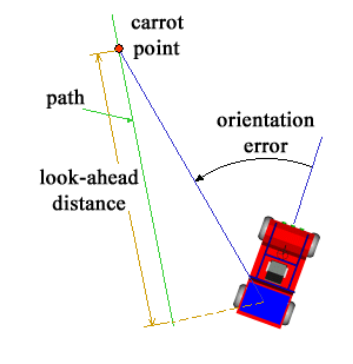
\includegraphics[height=5cm,keepaspectratio]{Chapter2/fig/FollowTheCarrot}
		\captionof{figure}{Follow the carrot}
		\label{fig:FollowCarrot}
	\end{minipage}%
	\begin{minipage}{.5\textwidth}
		\centering
		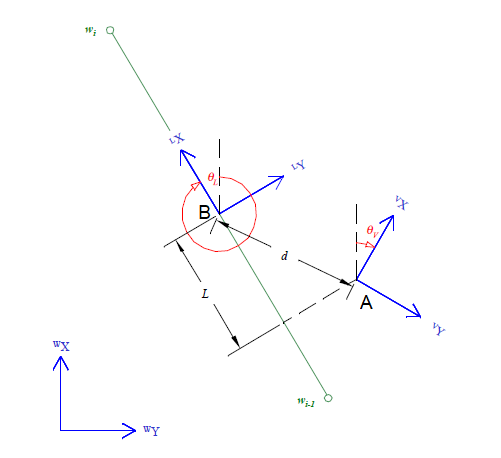
\includegraphics[width=1\linewidth,height=5cm,keepaspectratio]{Chapter2/fig/VectorPursuit}
		\captionof{figure}{Vector pursuit}
		\label{fig:VectorPursuit}
	\end{minipage}
\end{figure}
 The two previous geometric path tracking techniques  generate steering commands based upon the goal point on the reference trajectory to be traced. 
 %The requirement of vehicle posture control for accurate trajectory following remains unsatisfied.  
 Wit in \cite{wit2004autonomous} suggested a strategy to uses the path orientation and curvature  known at the goal point to improved path tracking,  such that the vehicle arrived at the goal point  with the correct orientation and curvature. Wit used Screw theory to find the error between the screw at the current location, point $A$  and the required screw at the goal position, Point $b$ as shown in Figure \ref{fig:VectorPursuit}. Control is then generated proportional to this error.

Hellstrom \cite{hellstrom2006follow} has proposed an algorithm which uses the knowledge of previously recorded steer angle, associated with  the path traced earlier. In this algorithm, the steer angle of the vehicle is set based on the orientation error, position error and the past recorded steer angle. A recent survey by Paden \cite{paden2016survey} provides extensive review of other control strategies for path tracking of autonomous unmanned vehicles such as those based on Lyapunov method, Model Predictive Controller, adaptive control, etc. 


   
\section{Tele-operation}
Tele-operation deals with  connecton of a   human operator with the robot in order to reproduce human action at distance. Tele-operation is in general bidirectional or bilateral as the human needs to have a feedback in order to understand the results of his action and to perceive the remote environment. It started with its use in nuclear and space industries \cite{martin1985teleoperated,vertut1986teleoperations}, but now it is used in underwater exploration, surgery, live-power line maintenance, mining, etc. All characterized by reducing the risk to human operators. The two major related research areas are the "human interface" and "control" design.
\subsection{Human interface}

Human interface is a means through which the operator interacts with the remote robot by perceiving the remote environment and sending commands accordingly. Thus, the human interface has two important purpose: one to excite the human senses to show the action of the executed task and to process the human command properly to execute it at the remote end.  Force and haptic feedback of remote environment drastically improves operator's performance. Hence a serial link haptic device PHANTOM \cite{massie1994phantom} was developed at MIT during 1994 to provide 3-DOF force feedback  for touch feedback purpose. DELTA Haptice Device described in \cite{grange2001overview} provides 6-DOF force feedback with moderate force. Clover \cite{clover1997dynamic} has reported  the use of off-the-shelf serial industrial robots for haptic realization of tasks requiring a large workspace and high force capability. Customized 10-DOF  haptic device was reported  for similar purpose in \cite{ueberle2004vishard10}. Design  of a 6-DOF parallel mechanism for force feedback is discussed in \cite{yoon2001design}.

Another major form of human interface is the visual feedback. The main challenge is to provide depth perception of remote environment. Most stereoscopic systems used in telerobotics are based on shutter glasses \cite{aracil1997telerobotic,matthies1992stereo}, head-mounted displays \cite{matthies1992stereo} or polarized images \cite{hirzinger1994robots}. Systems based on shutter glasses hide user's eyes alternately in synchronization to screen refreshment, which projects images for left and right eye alternately. A second type of interfaces is based on polarized images. The user is also required to wear glasses that filter the left and right images. The third type of interface is  the head mounted display such as "Google cardboard",  especially designed to immerse users into virtual environments where the left and right images are projected on each eye using two separate screens or split screens.

\subsection{Control}
Control of a tele-operetion system deals with two issues, \textit{transparency} and \textit{stability}. Transparency deals with what information is to be exchanged between the remote and local station so that the operator can have a natural feel of the remote environment. A position-position architecture is suggested by  Goertz \cite{goertz1961anl}, where  master position is passed as a command to the slave servo (position) controller, and slave position is returned to the master as a position command. A position-force architecture has been proposed by Flatau \cite{flatau1977sm} in which the master sends the position to the slave and the slave sends back the force felt by it in the remote environment. A general 4-channel architecture been suggested by Lawrence \cite{lawrence1993stability}, and transparency has been defined  as a measure of performance in teleoperation and evaluated for different architectures.
 
An excellent survey article on control of bilateral teleoperation was given by Hokayem and Spong \cite{hokayem2006bilateral}. Few of these are briefly presented here. A teleoperation system, comprised of a master and slave with their corresponding controllers, residing between the human operator and the environment,   can be modeled as a two port network. Passivity based design of stabilizing control using  wave-variable concept and scattering theory has been proposed by Anderson and Spong \cite{anderson1989bilateral}, Rebelo \cite{rebelo2015time} and Anderson and Slotin \cite{niemeyer1991stable}.   Port-Hamiltonian  based approach was used in \cite{stramigioli2010novel,stramigioli2005sampled}. Design of controller for time delayed systems  based on back-stepping method in combination with partial differential heat  equation was studied by  Kristic \cite{krstic2009delay}. 



\section{Predictive Display}
Delays are inherent in teleoperation over wireless network. Practically, much of the delay is due to relay stations and limited  bandwidth of the network.  As little as a half second delay in the visual feedback significantly reduces human performance \cite{chen2007human}. The operator tends to adopt an inefficient "move then wait and see" policy in order to complete the task.

    To overcome performance deterioration of the operator due to time delay in visual feedback, two approaches have been reported in the literature, namely, \textit{supervisory control or tele-assistance  } and \textit{predictive display}. In \textit{supervisory control} \cite{sheridan1986human,pook1994teleassistance,jagersand1995visual} the robot is partly guided by operator by giving the robot intermittent commands to achieve the goal. The drawback of such system is that operator looses direct contact with the task.
    In  predictive display systems, a natural and widely used techniques, synthesised view of the remote environment is displayed to the operator based on his movements. It has been used for space teleoperation as early as in 1993, which was reported by Sherdan \cite{sheridan1993space}, Bejczy \cite{bejczy1990predictive} and Kim \cite{kim1993demonstration}. Whereas the above two used a-prior modeling and  calibration of remote environment, Jagersand \cite{jagersand1999image} used delayed visual feedback and operator control signal to build predicated image which was presented to the operator. The system was implemented with a fixed remote environment with a manipulator arm with  two wall mounted cameras. An estimation function was proposed 
    $I_i \approx \phi_k(x_i), i \in {1,..k}$, that approximated each image  $I_i$ seen so far on the trajectory, i.e, ${x_1, x_2 .....x_k}$. Un-calibrated monocular camera mounted on manipulator (eye-in-hand) based image predication method was discussed   by Yeres \cite{yerex2003predictive} and Deng \cite{deng2003predictive}. Multiple sensors based dense 3-D  map of a remote scene was reported by Kelly \cite{kelly2011real} and \cite{burkert2004photorealistic}. While Kelly used fusion of  lidar and  camera,  Burkert used stereo cameras. Hu \cite{hu2015line} has used SLAM based Predictive Dispalay  (PD) system for telemanipulation of a mobile robot. In his approach, texture and geometry of the remote site was transmitted instead of  video stream. This, the author, claims reduces bandwidth utilization.
    \section{Summary}
    Different literatures relevant to the topic addressed in this research were presented. Each topic is a separate area of research in its self.  There are many more literatures in each topic which could be of great interest but was been skipped due to space constraints.  



\cleardoublepage
\chapter{Design of Mobile Platform}
\label{ch_3:KPI}
%The % Comment the below command to supress the random text
%\lipsum[3-20]
% % % % % % % % % % % % % % % % % % % % % % % % % % % % % % % % %

Most of the mobile robots presented in literature uses differential wheel drive  with passive castor, as in \cite{yamamoto1992coordinating}, \cite{rajendran2004} and \cite{saha1989kinematics}. The other  common methods for locomotion of mobile robots are the omnidirectional wheels  \cite{pin1994new} and \cite{salih2006designing}, and tracked wheel system \cite{suthakorn2009design} and \cite{guarnieri2004development}. According  to  Nagatani \cite{nagatani2000improvement},  a  vehicle  with  Mecanum  wheels  is  susceptible  to slippage and same is the case for tracked vehicle, which are inherently skid steered. The slippage of the wheels prevents the most popular dead-reckoning method using rotary shaft  encoders   from  being  performed  well. This chapter   discusses the  design methodology of a novel mobile manipulator based on environmental requirements. We also  highlight the advantage of the Davis steering mechanism over castor wheels  or other steering methods from the perspective of this mobile manipulator.   The Davis steering system modifies the heading of  front wheels in a way that, at low speeds, all the wheels are in pure rolling without lateral sliding \cite{wong2008theory}.  
%The kinematics and control of such systems are discussed in \cite{d1992dynamic} and references therein but no detail design is presented.  


\section{Design Overview}
 The objective of a  mobile robot under consideration is to navigate inside the cyclotron vault and collect radiation intensity data at all the required points decided by the operator. Data is to be collected not only at different planer locations of the floor but also at varying height from the floor. To cater to this operational requirement, a mobile platform with a vertically extendable manipulating arm was developed as shown in  Figures \ref{fig:robo3Dmodel} and \ref{fig:roboActual}. Together, they are   referred henceforth as mobile-manipulator. The 3-D model of the mobile-manipulator with its major subsystems are shown in Figure \ref{fig:robo3Dmodel}, whereas  and the actual   system  is shown in Figure  \ref{fig:roboActual}. 

 The environmental condition required that the vehicle be either  autonomous or teleoperated. To keep the complexity low it was decided to have wireless teleoperated   navigation and control. This gives an  operator full flexibility to drive  and control the system from a remote station  using  visual  feedback provided by the on board camera. The key parameters of the mobile manipulator are listed in  Table \ref{tb:specifications}.


 \begin{figure}
 	\centering
 	\begin{minipage}{.5\textwidth}
 		\centering
 		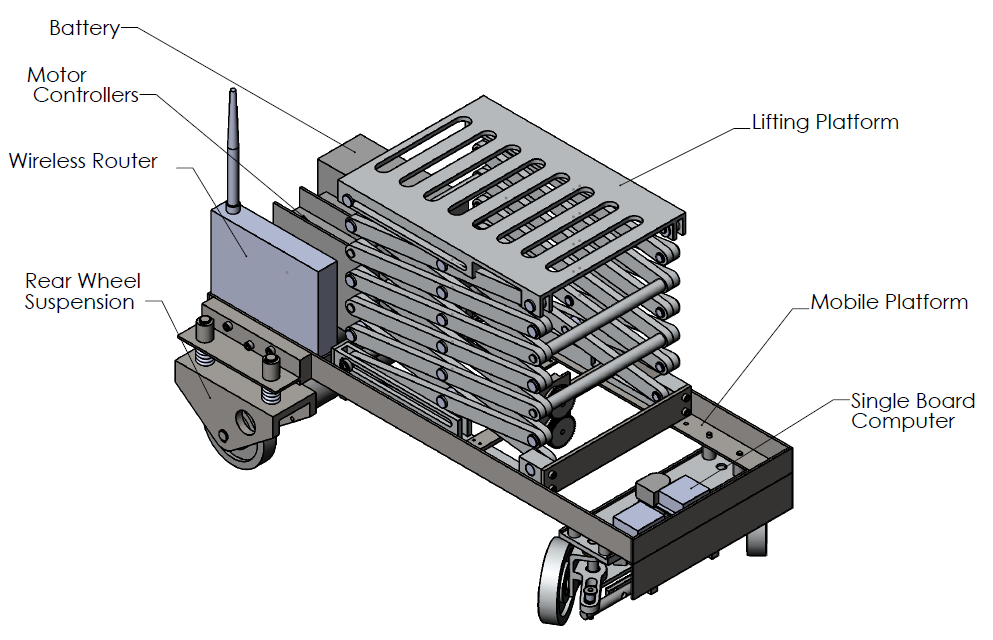
\includegraphics[height=5cm,keepaspectratio]{Chapter3/fig/robo3Dmodel}
 		\captionof{figure}{3-D Model of the mobile manipulator}
 		\label{fig:robo3Dmodel}
 	\end{minipage}%
 	\begin{minipage}{.5\textwidth}
 		\centering
 		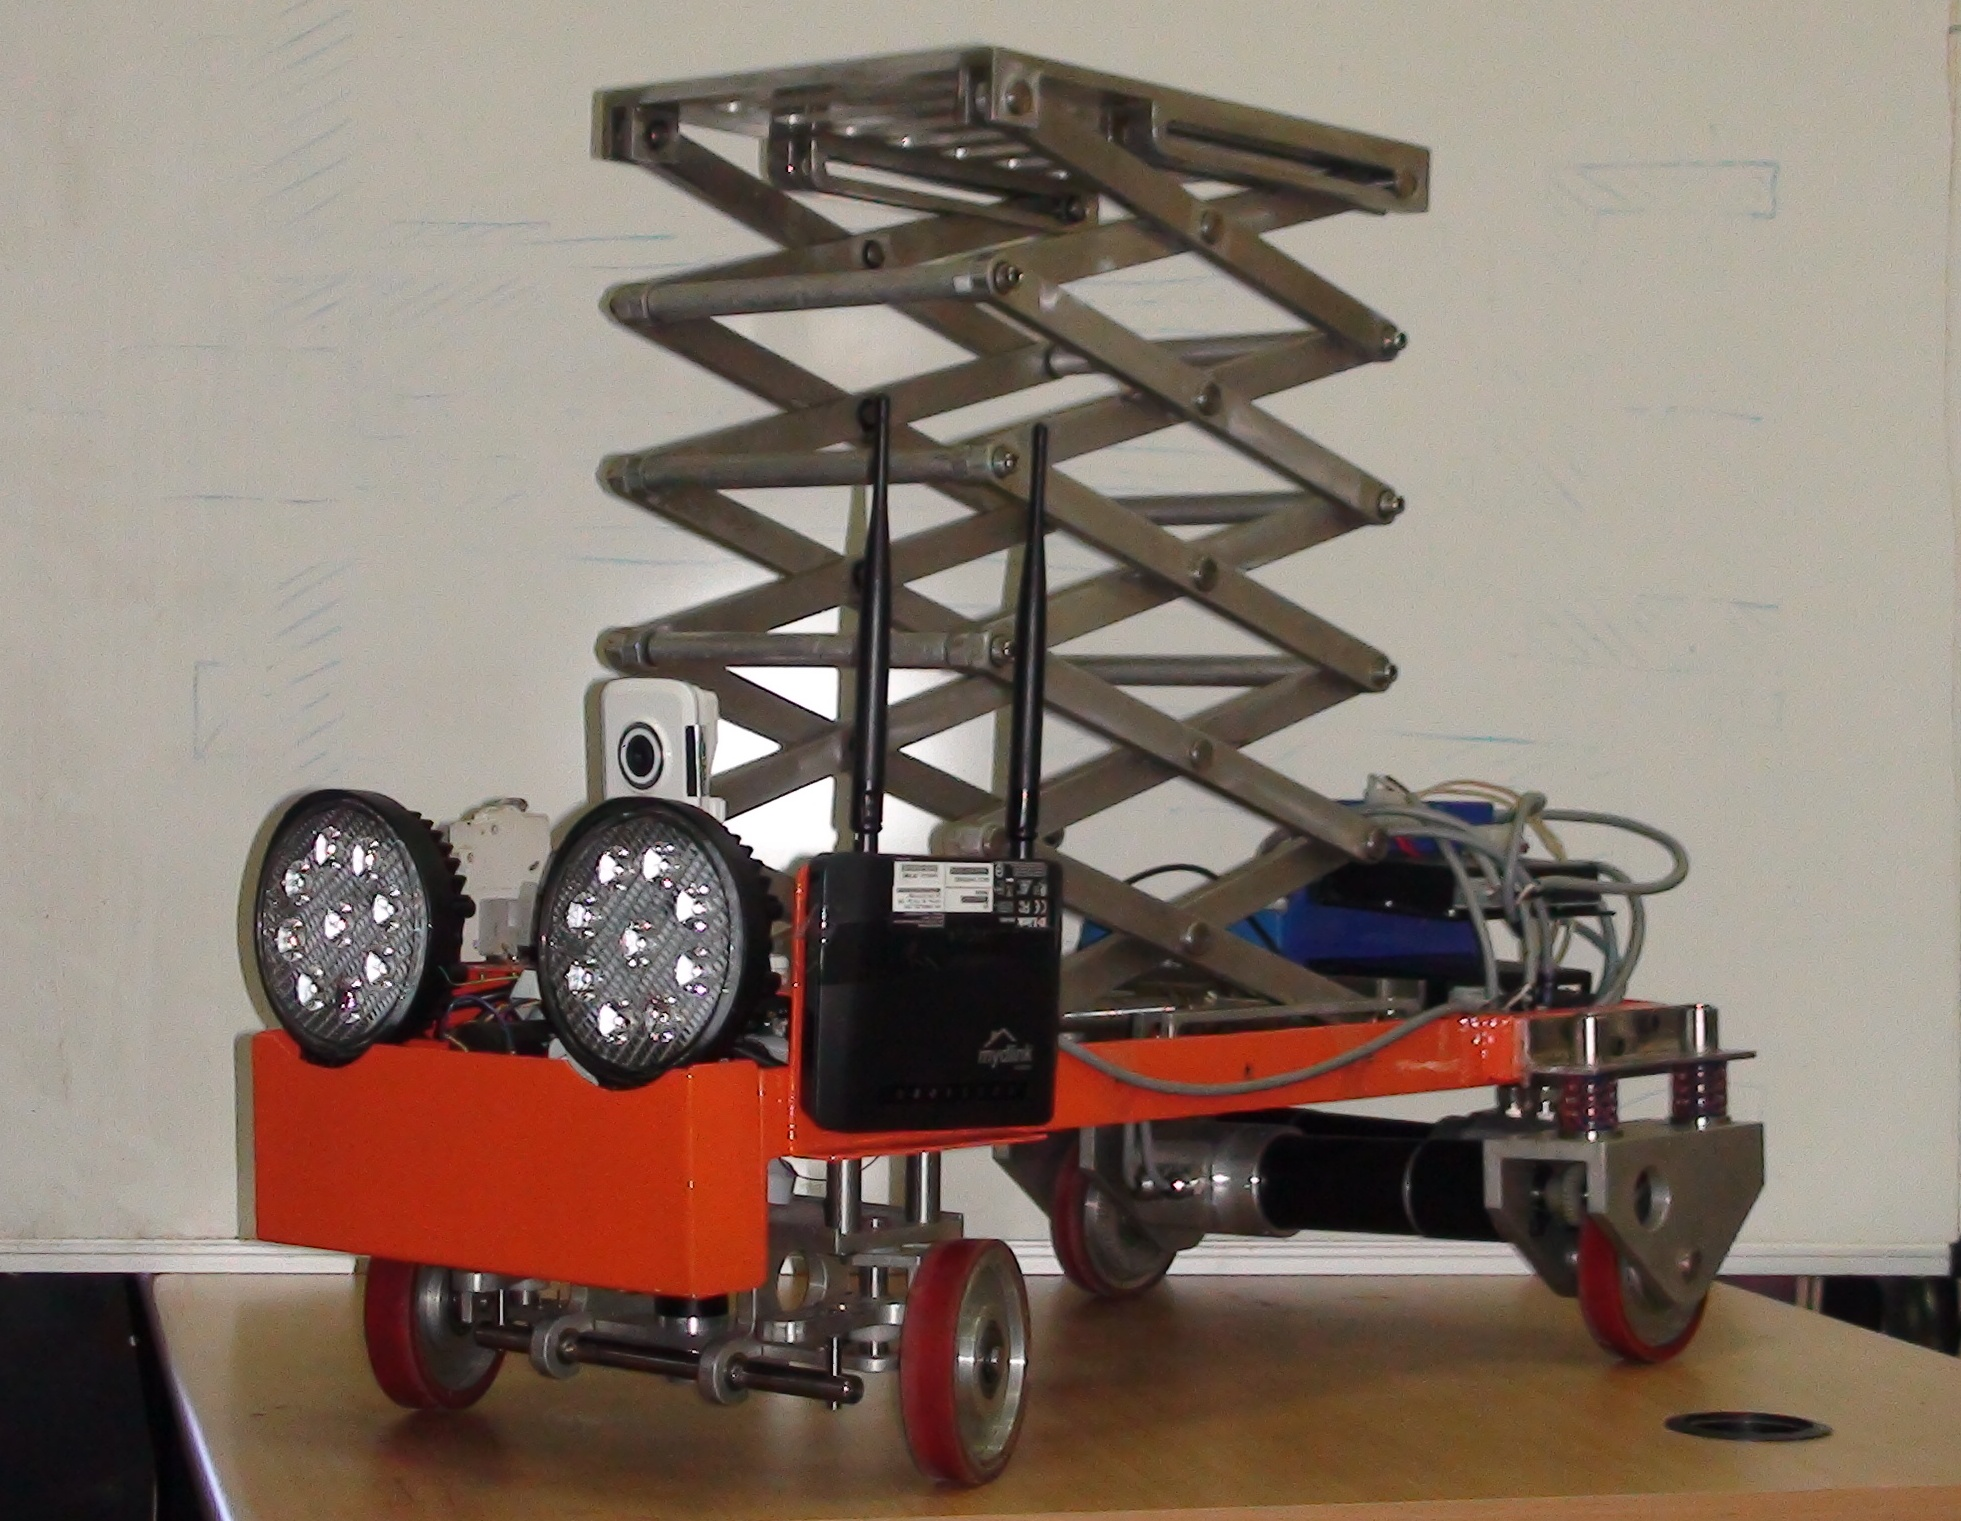
\includegraphics[width=.8\linewidth,height=5cm,keepaspectratio]{Chapter3/fig/roboActual}
 		\captionof{figure}{Photograph of the actual System}
 		\label{fig:roboActual}
 	\end{minipage}
 \end{figure}

%
\begin{table}[!htbp]
	\caption{Key parameters and specifications of the mobile manipulator.}
	\label{tb:specifications}
	\centering
	\begin{tabular}{l l l}
		\hline
		
		%\emph{Parameter}  & \emph{Example} & \emph{Font size and style} \\
		%\hline
		Weight  & 70 Kg & without payload \\ 
		Payload & 10 Kg &---\\
		Footprint & 700 mm $\times$  400 mm & - \\
		Height Collapsed & 500 mm  & Along  Z-Axis\\
		Height Extended & 1500 mm & Along  Z-Axis  \\
		Steering mechanism & Davis Steering & --\\
		Turning radius & 415 mm & - \\
		Ground clarence & 45 mm & --\\
		Maximum traction speed & 2 m/min & On flat terrain \\
		Ramp climb angle & $30^\circ $ & Checkerboard surface\\
		\hline
	\end{tabular}
\end{table}

The mobile-manipulator has a footprint of 700 mm x 400 mm  based on the narrow passage through which the system  has to negotiate. These passages are formed inside the vault area by the pipelines and  structural supports of the cyclotron and its associated equipment.  Two DC motors,with speed servo controller,  provide the traction to each rear wheels. The two front wheels are  inter-connected with a Davis steering mechanism \cite{TOMBook}. A scissor mechanism provides the vertical  motion of the detector that is mounted on the manipulating arm.

 In order to keep the self weight of the system small all the  structural parts are made of aluminum alloy AL6061, apart from the base frame. Stainless Steel (SS304)  angle sections was used for the base frame, which give it  excellent strength to weight ratio. 

\section{Design of the Traction System}
Traction is provided by the two rear wheels driven independently. This makes the system over actuated. A mechanical differential connecting the two rear wheels, as used in cars,  would overcome this. It was not proposed to do so as the proposed vehicle is planned to be teleoperated in a environment inaccessible to humans. This calls for a single-failure-safe design. The proposed design gives two major advantages. 
Firstly, in case  one of the wheel loosing contact with the ground due to  overhang in small pits or while over an obstacle, the mechanical differential system would keep supplying power to the free hanging wheel. The system will hence get stuck, maybe in an unrecoverable location. This situation is avoided in the present design as the motor having traction can be independently powered, to move the vehicle.  
Secondly, using the proposed design, in case of one  actuator failure, either the traction or the steering motor, still the vehicle can be manoeuvred to a  safe location, albeit with dragging of the wheel with failed actuator.

    Each wheel is driven by a  Maxon DC RE50 200W Motor through a 26:1 reduction gearbox. The motors are mounted at an offset to the wheel axis for increased ground clearance, as shown in Figure \ref{fig:tractionDrive}. Spring suspension is provided at each wheel to ensure sufficient contact force on uneven  ground. The diameter of the wheel is 100 mm $(D_w)$, which is sufficient to ride over obstacle of height 20 mm (Max). They are made of Aluminum alloy-6061 with 5mm thick molded polyurethane (PU) liner. The PU liner provides large traction on cement flooring while being resistance to wear.

  The load distribution was optimized to generate maximum normal reaction, $F_n$,  at the rear wheels without overturning while moving up the ramp of $30^o$. Maximizing rear wheel reaction by increasing  "b" as per Equation \ref{eqn:loadratio} ensures increased traction, $F_T=\mu F_N$ ($\mu$ is the coefficient of friction), but at the same time decreases the stability margin indicated by "X" in Figure \ref{fig:loadDistribution}. The static moment and force balance yield
\begin{equation}
\label{eqn:loadratio}
F_{N2}=\frac{b}{a}F_{N1}, \quad F_{N1}+F_{N2}=mg\cos\theta
\end{equation}

The stability margin $X$ as shoen in Figure \ref{fig:roboActual} was fixed as $30mm$ so as to achieve  maximum acceleration of $0.144g$  over the ramp of $30^o$ without overturning. This was done based on the condition of dynamic stability given by
\begin{equation}
\label{eqn:overturn}
mgb\cos\theta=(mg\sin\theta+ma)z_{cg}, \quad \Rightarrow g(\frac{b}{z_{cg}}\cos\theta-\sin\theta)=a
\end{equation}


Where 
\begin{itemize}
\item[] $F_{N1}$, $F_{N2}$ are normal reaction on the front and rear wheels.
\item[] a and b are the distance of the vehicle cg from the rear and front wheels.
\item [] $Z_{cg}$ is the height of the cg from the  plane containing the contact point of the wheels.
\item [] $m$ is mass of the vehicle.
\item [] $g$ is acceleration due to gravity.
\item[] $\theta$ is the inclination of the traction surface from horizontal.
\end{itemize}


 
\begin{figure}
 	\centering
 	\begin{minipage}{.5\textwidth}
 		\centering
 		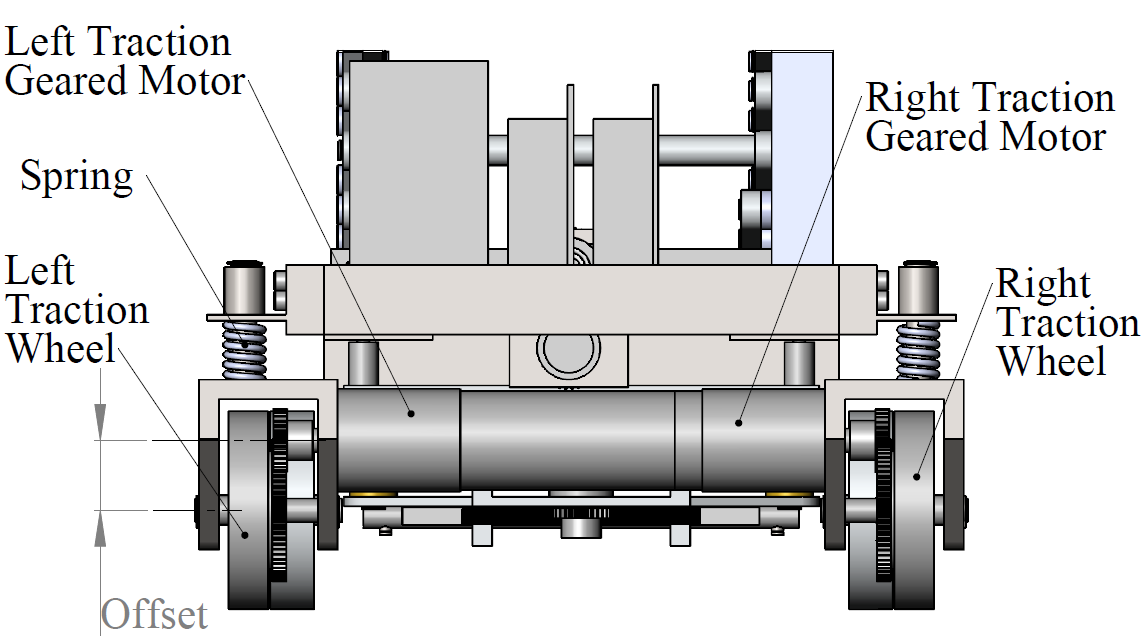
\includegraphics[width=.9\linewidth,height=4.5cm,keepaspectratio]{Chapter3/fig/WheelOffset}
 		\captionof{figure}{Rear Suspension}
 		\label{fig:tractionDrive}
 	\end{minipage}%
 	\begin{minipage}{.5\textwidth}
 		\centering
 		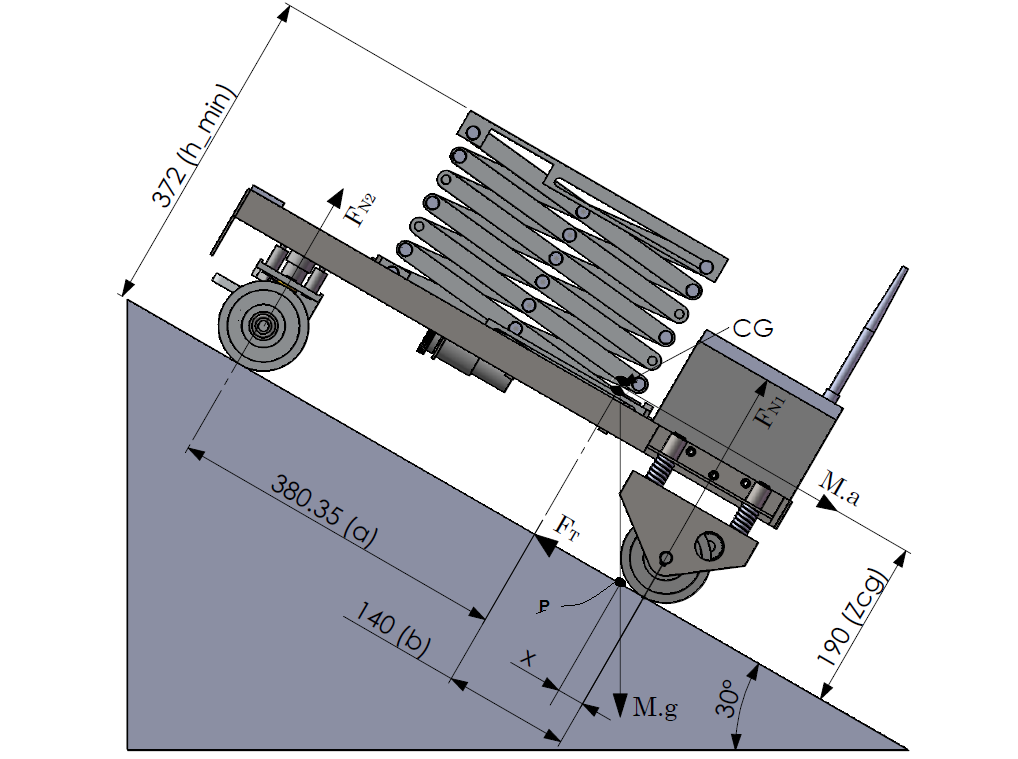
\includegraphics[height=4.5cm,keepaspectratio]{Chapter3/fig/loadDist}
 		\captionof{figure}{Mobile Manipulator on slope}
 		\label{fig:loadDistribution}
 	\end{minipage}
 \end{figure}
 \subsection {Selection of Motor and Gearbox}
 The torque requirement for each rear wheel was calculated based on the static moment balance with the assumption that each rear wheel shares equal load and the total suspended weight is 80 Kg. From the freebody diagram (Figure   \ref{fig:loadDistribution}), using moment and force balance  we get the following:
\begin{equation}
\label{eqn:t1}
F_{N1}=\frac{a M \cos \theta}{a+b-\mu Z_{cg}} , \quad \quad
F_T=\mu F_{N1}
\end{equation}
In order to estimate the traction motor size, we take worst case scenario of $\theta=30^o$ and $\mu =0.3$. This leads to
\begin{equation*}
F_{N1}=66 Kg, \quad\quad F_T=0.3*66 \approx 20Kg
\end{equation*}
 Since the traction is provided by the two rear wheels, the torque required per wheel $(T_w)$ is given by
\begin{eqnarray}
T_w=(F_T/2)(D_w/2)= (20/2)*50=500 Kg-mm \simeq 5 Nm
\end{eqnarray}
The motor torque $T_M$, required based on the assumption of factor of safety, $FS=1.5$ is
\begin{equation}
T_M=(FS)*T_w=1.5*5 =7.5 \simeq 8Nm
\end{equation}
 Assuming the maximum speed, $V_{ramp}=1m/s$, of the mobile manipulator over a ramp, the required power, $P_M$, of the traction motor is calculated as,
 \begin{equation}
 \begin{aligned}
\omega_w&=V_{ramp}/(D_w/2) \simeq 200rpm\\
P_m&=\omega_w T_m=20*8=160W
 \end{aligned}
 \end{equation}
 The nearest Maxon motor available as per the catalogue \cite{catMaxon} is 200W,  RE50-370354 motor.  The nominal speed, $N_s$ is 5680rpm. Therefore, the  gearing  ratio required is, $N_s/\omega_w=5680/200 \simeq 28.4$. The nearest gear box available  is of ratio $26:1$, which was chosen. 

\section{Design of Steering System }
The design objective of a steering system should ensure rolling motion of all the  wheels during every possible manurers of the mobile robot. This is important to reduce the friction drag due to sliding motion which reduces the energy efficiency of the mobile robot. In case of four wheeled vehicle with rear wheels fixed and front wheels steered the condition is  shown in Figure \ref{fig:steerCond},  referred in some literature as Ackerman steering conduction.   

This mobile manipulator uses Davis steering mechanism,  Figure \ref{fig:davis},  on the front wheels. Caster wheels  were not used as they tend to align with  obstacles and thus get stuck. On the  other hand tracked wheels have excellent rough terrain capabilities, but is power intensive due to skid steering. another option was to use   Omnidirectional wheels, which need complex controller for coordination and an extra actuator. Moreover, the operation are are in general not clean of loose small objects, which may get stuck in between the free rollers of the omnidirectional wheels. This will reduce the efficiency of the vehicle.  

\begin{figure}
 	\centering
	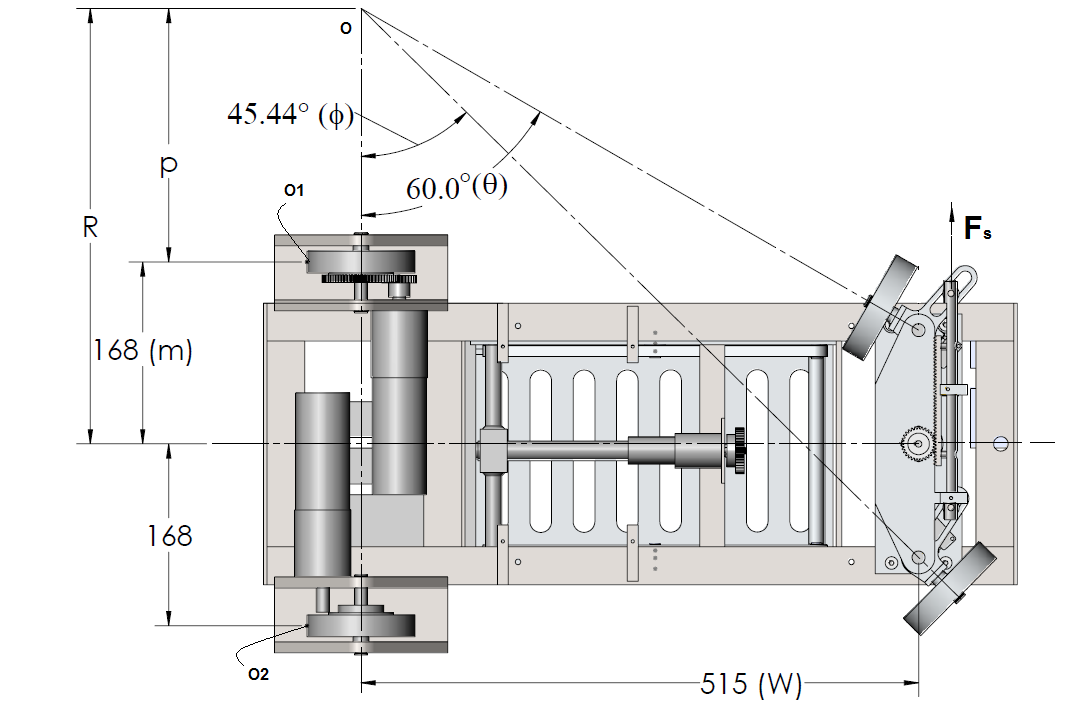
\includegraphics[width=\linewidth,keepaspectratio]{Chapter3/fig/steerringCondition}
	\captionof{figure}{Ackerman Steering Condition }
	\label{fig:steerCond} 
\end{figure} 
 

Davis mechanism was chosen over Ackerman steering gear as it satisfies the steering condition given by  Equation \ref{eqn:Acker}, which ensures pure rolling of all  wheels over the entire steering range. This makes the system suitable for passive wheel odometry and energy efficient.  The mechanism being positively driven by position controlled servo motor does not align with the obstacles and thus are able to crossover it. The dimensions of the links used in the steering mechanism is given in Figure \ref{fig:davis}, and are based on the Ackerman steering law given below:
\begin{equation}
\label{eqn:Acker}
\cot\phi-\cot\theta=a/w, \quad  \frac{2b}{h}=\frac{a}{w}
\end{equation}
Where $a$ and $b$ is limited by the over all size of the vehicle, discussed earlier.

\subsection{Minimum Turning Radius}
The mechanical construction of this steering mechanism limits the steering angle. This in turn limits the minimum radius the vehicle can negotiate.
Figure \ref{fig:steerCond} shows the extreme values of $\phi$ and $ \theta$, one side of the steering limits. The \textbf{ turning radius } $R$ for a given steer angle $\theta$  is calculated  by the geometry of Figure  \ref{fig:davis} as
\begin{equation*}
\tan\theta =\frac{w}{P+m-\frac{a}{2}} \quad \text{and} \quad R=m+p
\end{equation*}
Substituting $R$ and rearranging the above equation, we get 
\begin{equation}
\label{eqn:turningRadius}
R(\theta)=\frac{a}{2}+w\cot\theta
\end{equation}
The extreme value of $\theta=60.$ as shown in Figure \ref{fig:steerCond}, this gives the \textit{minimum turning radius } $R_{min}$ as
\begin{equation*}
R_{min}=\frac{210}{2}+515 \times cot(60^o)=402mm
\end{equation*}

\begin{figure}
	\centering
	\begin{minipage}{.5\textwidth}
		\centering
		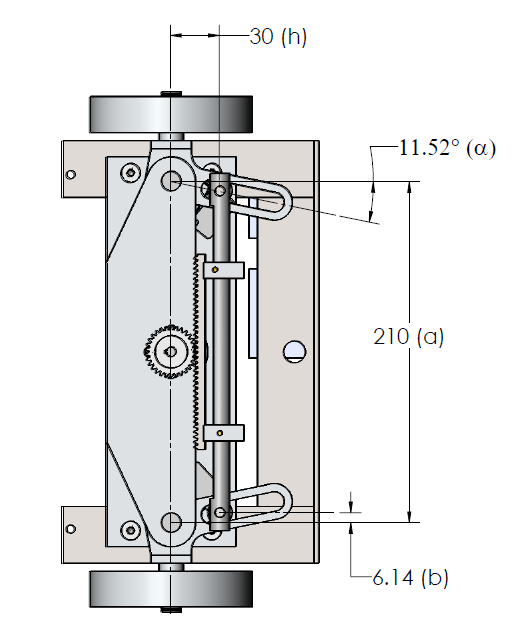
\includegraphics[width=\linewidth,height=5cm,keepaspectratio]{Chapter3/fig/davis}
		\captionof{figure}{Davis Steering Gear}
		\label{fig:davis}
	\end{minipage}%
	\begin{minipage}{.5\textwidth}
		\centering
		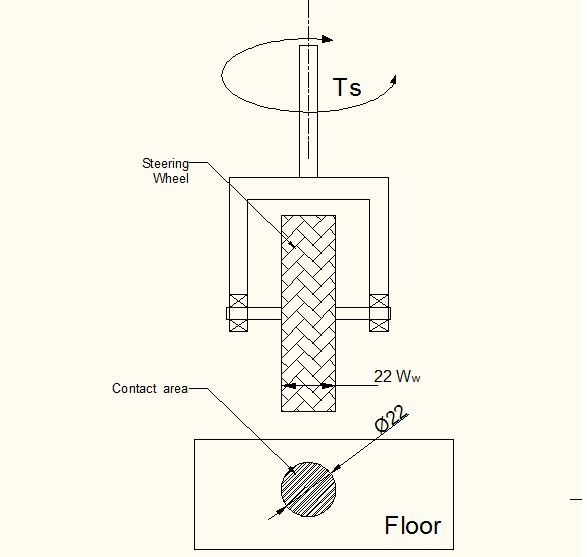
\includegraphics[width=\linewidth,height=5cm,keepaspectratio]{Chapter3/fig/steerTorqCal}
		\captionof{figure}{Steer Torque}
		\label{fig:steerTorq}
	\end{minipage}	
\end{figure} 

\subsection{Calculation of Steering Torque}
The torque required to steer the front wheel is estimated based on a simplified assumption that the wheel deforms under normal load and the contact area thus generated is  circular in shape with diameter that of the wheel width, $W_w$, as shown in Figure \ref{fig:steerTorq}. 
In order to estimate the normal reaction on each wheel, we assume that the total weight of 80kg is equally shared by the four wheels. 
Therefore, $N_s=80/4=20Kg$. Next, the uniform pressure formula used for  brakes/clutches design was applied to find the resistance  torque $T_s$, between the ground and the wheel i.e, 
\begin{equation}
\label{eqn:brake}
T_s=\frac{N_s\mu}{3}W_w= 0.4Nm
\end{equation}  
The resistance torque, $T_s$, of  both the wheels  are balanced by the force $F_s$ acting on the rack as shown in Figure \ref{fig:davis}. The rack is coupled to the steering motor by a pinion of diameter, $D_p=40mm$. The motor  torque, $T_{m_s}$  in Equation  \ref{eqn:SteerTq} is calculated with a  high factor of safety, $FS=3$. This is because $T_S$ is estimated  based on a simplified model of brake design. The power, $P_{m_s}$ of the steering motor based on  torque $T_{m_s}$ and the steering speed $\omega_s$ of 100rpm is 
\begin{equation}
\begin{aligned}
\label{eqn:SteerTq}
T_{m_s}=(FS)\frac{2T_s}{h}\frac{D_p}{2}=1.6Nm \quad \text{and}\quad P_{m_s}=T_{m_s}*\omega_s=17W
\end{aligned}
\end{equation} 

Based on the above specifications, a 20W, RE25 DC motor of Maxon  make and a gear box  GP32 of ratio 159:1 was chosen for the steering mechanism. 
 
\section{Design of Scissor Mechanism for Manipulating Arm}
 The manipulating arm  was designed to move  up to a height of 1.5m from the floor level. This motion was generated using  a scissor mechanism, as shown in Figure \ref{fig:scissor}. The scissor mechanism has two major advantages over other lifting methods such as telescopic pillar, etc.  First, the  ratio of height in extended and collapsed condition is very large. In our case it is $3:1$. Second, the self weight of the mechanism is less as it is made of rectangular links.

The scissor mechanism, Figure \ref{fig:scissor}, has 6 stages, where one "X" denotes one stage. 
\begin{figure}
	\centering
	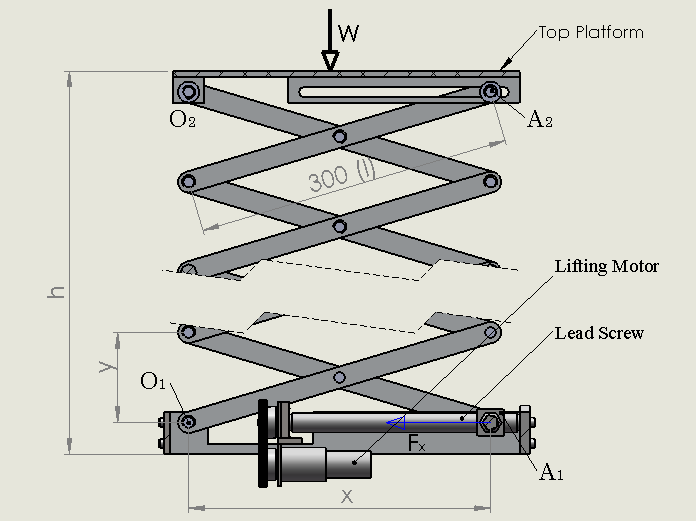
\includegraphics[width=\linewidth,keepaspectratio]{Chapter3/fig/scissor}
	\captionof{figure}{Scissor Mechanism}
	\label{fig:scissor}
\end{figure}
The Scissor is connected to the top platform by a pivot joint $O_2$ and a prismatic joint $ A_2$.
 This is coupled to the base frame by pivot joint $O_1$ and a prismatic joint $A_1$. The linear actuation of joint $A_1$ is provided by a lead screw of pitch ($P$) 1.5 mm and mean diameter ($d_m$) 10mm.
  This results in vertical motion of the top platform. 
  
 The relation between the vertical motion of the platform and the horizontal displacement of point $A_!$ is given by geometry of the mechanism shown in Figure \ref{fig:scissor} 
\begin{equation}
\begin{aligned}
y&=l\sin\theta,\; x=l\cos\theta,\; \Rightarrow dy=l\cos\theta d\theta, \; dx=-l\sin\theta d\theta\\
h&=Ny\rightarrow dh=Ndy
\end{aligned}
\end{equation} 
where $l$ is the link length, $\theta$ the angle of the link with horizontal plane and $h$ the height of platform.


The number of stages used in the scissor mechanism is N=6. From the principle of virtual work, we get 
\begin{equation}
\label{eqn:ScissorForce}
\begin{aligned}
-F_xdx=Wdh,\;\Rightarrow F_x=\frac{WN}{\tan\theta}
\end{aligned}
\end{equation}
where, $F_x$ is the axial force on the prismatic joint, $A_1$ and W is the payload. From Equation \ref{eqn:ScissorForce}, it is clear that as $\theta\rightarrow 0$, the force  $F_x \rightarrow \infty$. In the present design,  $\theta_{min}=5^o$ and $\theta_{max}=45^o$. Therefore, the extended height  $h_{max}=Nl\sin\theta_{max}=1.3m$ and the collapsed height $h_{min}=156mm$. Assuming $W=8kg$ as payload the maximum force $F_x=342Kg$ is required at $\theta_{min}=5^o$, . 

The motor torque required for the scissor mechanism is calsulated using  screw jack formula given in  \cite{TOMBook} and here presented as Equation \ref{eqn:liftingTorque}. 
\begin{equation}
\label{eqn:liftingTorque}
\begin{aligned}
T_L&=\frac{F_x d_m}{2}(\frac{p+\pi\mu d_m\sec\alpha}{\pi d_m-\mu p\sec \alpha})=7.5Nm
\end{aligned}
\end{equation}
where coefficient of friction assumed, $\mu=0.1$, ACME thread angle $2\alpha=60^o$, pitch diameter $d_m=15mm$ and pitch $p=1.5mm$ is used. Based on the above specification 10W RE20 DC motor with a gear box of 25:1 ratio was chosen from Maxon motor catalogue ~\cite{catMaxon}.



  
  

\section{Summary}
Design calculations for the proposed  mobile manipulator are presented in this chapter. Different aspects based on the requirements of radiation inspection around cyclotron was taken into account. Advantage of positively steered wheels over caster wheel was highlighted for the proposed mobile robot. 

%-------------------------------------------------------------
%\bibliographystyle{ieeetr} %bibliography style-file
%\bibliography{sample} % bibliography database file


\cleardoublepage
\chapter{Dynamics of Wheeled Mobile Robots }
\label{c4_Dynamics}
In the field of mobile robotics, extensive research has been carried out. 
Mobile robots can broadly be divided into three categorises, namely wheeled robots, legged robots ~\cite{machado2006overview}, and aerial vehicles ~\cite{valavanis2014handbook}. 
There are few mobile robots which use both wheels and legs for locomotion. For example,  Creadapt  \cite{mouret2015evolutionary} in order to take advantage of both modes of locomotion. 
Among these, the most extensively studied are the  Wheeled Mobile Robots (WMR). 
They have been classified into five generic classes by Champion et. al. \cite{campion1996structural},~\cite{campion2008wheeled}  based on their mobility resulting from the kinematic constrains due to  different wheel types.
 The most common among these are the  3 wheeled differentially driven WMR with one castor wheel.
  Because of its simplicity in modelling, they have been used in most of the  control and motion planing algorithms  \cite{desantis1995modeling}, \cite{koh1999smooth} and \cite{d1995control}. 

In order to develop a model-based control algorithm, it is imperative to have a good dynamic model of the WMR.
 These dynamic models are used in  simulation software,  Software in Loop (SIL) testing and Hardware in Loop (HIL) testing  of the controllers.
 Different methods have  been adopted to derive the dynamic model of WMRs.
  A general dynamical model was derived for three-wheel mobile robots with nonholonomic constraints  by B. d'Andrea-Novel \cite{d1991modelling} using  Lagrange formulation.
    Alternatively, Thanjavur and Rajagopalan \cite{thanjavur1997ease} have used Kane's method,  and  Saha et al. \cite{saha1991dynamics},\cite{saha1989kinematics} used Natural Orthogonal Compliment (NOC) method for the same.  
    
In this chapter we first present the kinematic model of the mobile robot with two passive wheel at the front. It is then proved using kinematics why a passive wheel with caster offset along the plane of the wheel self orients itself. while  casters with zero offset  must be actuated.  This has not been explicitly presented in literature.

 Next the dynamic equation of a mobile robot using Natural Orthogonal Compliment method is derived for both for ideal rolling condition of wheels and in presence of longitudinal and lateral slip of wheels. Use of NOC for modeling differential drive wheeled vehicle under ideal rolling condition as been presented by Angels and Saha \cite{saha1991dynamics}, \cite{saha1989kinematics}. We extend this method to include both the lateral and longitudinal slip of the wheels, and  derive the dynamic equations of motion of a mobile robot with redundant actuators. 
 
 The RARS robot has a unique  drive configuration, which uses both differential drive and Davis mechanism for steering. 
 This system has a redundant configuration and very few literature presents dynamical analysis with slip included in the dynamics. To our knowledge no literature is present, where the concept of  NOC  has been used to model redundantly actuated mobile robot. The two models are compared using simulation to find the deviation in the path traced by RARS robot under different peak value of co-efficient of friction between the wheel and ground plane.
   


   
 
 

  
  
  
  
  
\section{Modeling using the Natural Orthogonal Compliment (NOC)}
Let us consider a system with $n$ rigid bodies interconnected with different types of joints. 
Let, $f_i$ be the net force acting at the center of mass (CM) of the $i^{th}$  body and $n_i$ is the net moment.
 If $m_i$ is the mass, $I_{ci}$ is the  moment of inertia with respect to the CM, $c_i$ is the position vector of the CM and $\omega_i$ is the angular velocity of the same body, then equations of motion of the $i^{th}$ rigid body are given by Newton-Euler equations as 
\begin{equation}
\label{NE}
f_i=m_i\ddot{c_i} \quad and \quad n_i=I_{ci} \omega_i+\omega_i \times I_{ci} \omega_i
\end{equation}
Let us  define twist ($t$) and wrench($w$) as 
\begin{equation*}
t_i \equiv \begin{pmatrix}
\omega_i\\ \dot{c_i}
\end{pmatrix} \quad
w_i \equiv \begin{pmatrix}
n_i\\f_i
\end{pmatrix}
\end{equation*}
Note that the wrench $w_i$ acting on the $i^{th}$ body can be decomposed into $w^w_i$, called the \textit{working component} and  $w^c_i$, the \textit{non-working component}.
 The working component consists of all the external  moments and forces, which imparts/extracts energy to/from the system, e.g., motor actuating torque.
  The non-working component of the wrench consists of the moments and forces that are used to constrain the motion of the body at the joints.
Then, Newton-Euler equations (\ref{NE}) can be rewritten  in a single matrix equation as 
\begin{equation}
\label{2}
M_i\dot{t_i}+W_iM_it_i=w^w_i+w^c_i \quad \because w_i \equiv w^w_i+w^c_i
\end{equation}
where
\begin{equation}
\label{3}
M_i \equiv \begin{pmatrix}
I_{ci} & 0\\0 & m_i\tilde{1}
\end{pmatrix} ,
\quad W_i\equiv \begin{pmatrix}
\Omega_i &0\\0&0
\end{pmatrix},
\quad
\Omega_i\equiv \omega_i\times \tilde{1}
\end{equation}
in which  $\Omega_i$, is refered as the cross-product matrix of vector $\omega_i$ and $\tilde{1}$ denotes the identity matrix.For details, refer to \cite{angeles2013fundamentals},\cite{saha2010robotics}.If we define 
\[M \equiv diag[M_1,M_2,...M_n], \quad W \equiv diag[W_1,W_2,...W_n], \quad t \equiv [t_1^T,t_2^T, ....t_n^T]^T\] 
and 
\[ w^j \equiv [{w_1^j}^T,{w_2^j}^T, ....{w_n^j}^T]^T, \,j=c,w \]
then the equations of all the $n$ rigid bodies in the system can be collected and written as a single matrix equation 
\begin{equation}
\label{DCE}
M\dot{t}+WMt=w^c+w^w
\end{equation}
 The above equation is referred to as  decoupled equations of motion of the system.



The kinematic constraints, both holonomic and non-holonomic (e.g., pure rolling), between two bodies $i$ and $j$ of a system can be expressed as a linear homogeneous system of algebraic equations \cite{angeles2013fundamentals}, namely 
\begin{equation}
A_it_i+A_jt_j=0
\end{equation}
where $A_i,A_j$ depend on the kinematic parameters.

The constraint equations corresponding to all the joints in the system can be written in terms of the \textit{generalized twist vector} $t$. Furthermore, if $ \dot{\theta} \equiv[\dot{\theta_1},\dot{\theta_2},...\dot\theta_n]^T$ denote the \textit{independent generalized joint rates}. One can then write $t$ in terms of $\dot{\theta}$ as $t=T\dot{\theta}$. 
Using the fact, that $\dot{\theta}$ can take any arbitrary value, we get
\begin{equation}
\label{AT}
At=0 , \quad \Rightarrow  AT\dot{\theta}=0\quad \Rightarrow AT=0
\end{equation}
The Equation \ref{AT} indicates that $T$ is the orthogonal complement of $A$.
 Since this relation arises naturally, hence the name \textit{Natural Orthogonal Complement}.  It can be shown \cite{angeles2013fundamentals} that the non-working wrench $w^c$ lies in the range space of $A^T$.   In view of Equation \ref{AT}, it can be proved that $w^c$ lies in the null space of $T^T$. Therefore,
\begin{equation}
T^Tw^c=0
\end{equation}
To eliminate the non-working  moments and  forces, i.e., $w^c$ from the uncoupled equation of motion (\ref{DCE}), we multiply both sides of the equation  by $T^T$,
\begin{equation}
 T^TM\dot{t}+T^TWMt=T^Tw^W, \quad
 \Rightarrow T^TMT\ddot{\theta}+T^T(M\dot{T}+WMT)\dot{\theta}=T^Tw^w
 \label{eqn:CEM}
\end{equation}
Equation \ref{eqn:CEM} represents the dynamic equation of  interconnected $n$-body system.
 This equation is expressed in terms of the independent generalized joint rates $\dot{\theta}$ and cosponsoring  acceleration $\ddot{\theta}$. Further, using the relations $t=T\dot{\theta}$ and $\dot{t}=\dot{T}\dot{\theta}+T\ddot{\theta}$  in Equation \ref{eqn:CEM}  the final equations of motion can be written as

\begin{equation}
\label{CE}
 \quad I(\theta)\ddot{\theta}+C(\theta,\dot{\theta})\dot{\theta}=\tau
\end{equation}
where
\begin{align*}
I(\theta) &\equiv T^TMT\quad \quad:\text{generalized inertia matrix}\\
C(\theta,\dot{\theta})&\equiv +T^T(M\dot{T}+WMT) \quad :\text{generalized  convective inertia matrix}\\
\tau&\equiv T^Tw \quad \quad :\text{ generalized vector of driving forces }
\end{align*}

Where, 
\begin{equation}
	I(\theta)=\sum_{i=1..n}(T_i^TM_iT_i)
\end{equation}
\begin{equation}
C(\theta,\dot{\theta})=\sum_{i=1..n}(T_i^T M_i\dot{T_i}+T_i W_i M_i T_i)
\end{equation}
\begin{equation}
\tau=\sum_{i=1..n}T_i^T w^w_i
\end{equation}

\begin{figure}
	\begin{minipage}[t]{0.5\textwidth}
	\centering
		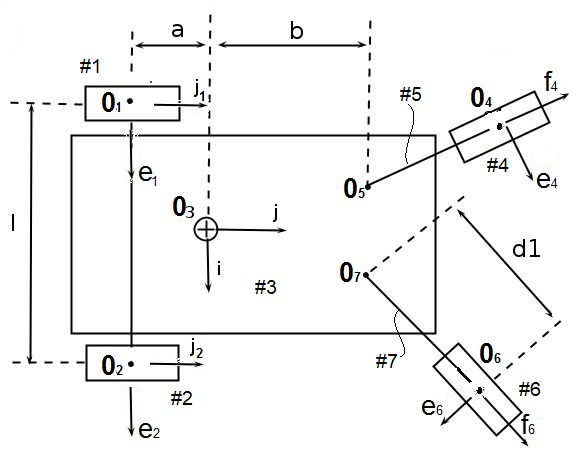
\includegraphics[width=3in]{Chapter4/fig/fig1.jpg} 
		\caption{WMR-Std. caster}\label{fig:std}
	\end{minipage}
	\hfill
	\begin{minipage}[t]{0.5\textwidth}
	\centering
		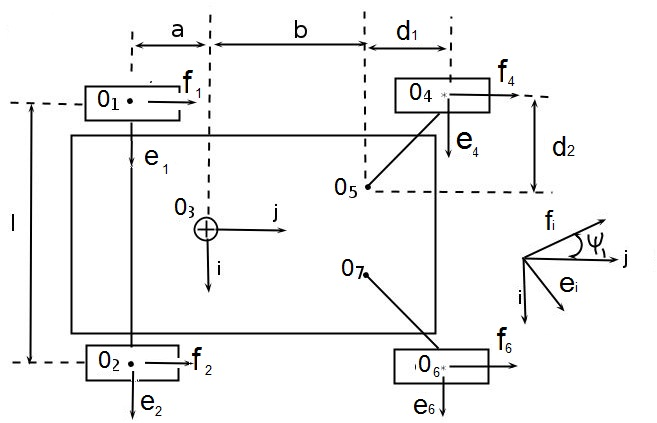
\includegraphics[width=3.5in]{Chapter4/fig/fig2.jpg} 
		\caption{WMR-general}\label{fig:gen}
			\end{minipage}
%\caption{Castor wheel configuration of a WMR}
\end{figure}


\section{Dynamic Equation of WMR}
\label{sec:DynamicNoSlip}
The dynamic equation of a differentially driven 3 wheeled mobile robot based on the  Natural Orthogonal Compliment (NOC) has been presented by Saha~\cite{saha1991dynamics}. The vehicle consisted of 2 driven wheels and one standard caster wheel. In general, for large vehicles, it is necessary to have at least four wheels from the point of stability of the vehicle. Such a vehicle  is shown in Figure \ref{fig:std}. It may be noted that the caster wheels used in this case are the standard caster, where the angle between line $O_4O_5$ and vector $e_4$ is  $90^o$. Which is a special case of the more general configuration of the passive wheels shown in figure \ref{fig:gen}, where angle between line $O_4O_5$ and vector $e_4$ is not $90^o$

 The vehicle considered for analysis in this chapter is shown in Figure \ref{fig:gen}. It consists of two independently driven wheels at the back and two passive wheels at the front. The actuated wheels are labelled as body \#1 and \#2 as indicated in Figure \ref{fig:gen}. The platform is body \#3. The first caster wheel and its bracket is labelled as \#4 and \#5 respectively, with the castor pivoted at $O_5$. Similarly, the second castor is pivoted at $O_7$, and its bracket and wheel are labelled as \#6 an \#7, respectively, all the wheels are assumed to be rolling without slipping.  
 
 The RARS robot wheel configuration can be arrived from the generalized configuration of caster wheels presented above when $d_1=0$. Under this condition the and assuming that the steering mechanism always provides the correct steer angle, which is true in case of small curvature paths, the dynamic behaviour of the proposed robot will be similar to that  shown Figure  \ref{fig:gen}.
\subsection{Kinematic analysis}
In order to proceed with the kinematic analysis of the vehicle in Figure \ref{fig:gen}, we define an orthogonal triad of vectors ${i,j,k}$ at point $O_3$, the control point of the platform, as shown in Figure \ref{fig:gen}. If $\dot{\theta_1}$ and $\dot{\theta_2}$ {( positive when pointing along $i$)} denote the rates of rotation of wheels \#1 and \#2 then the linear velocity of points $O_1$ and $O_2$ under pure rolling condition is given by 
\begin{equation}
\label{velO1}
{\dot{o_i}}=-r\dot{\theta_i}j, \quad \text{r=radius of wheel}
\end{equation}
The angular velocity of the platform $\omega_3$ can be written as 
\begin{equation}
\label{omegaPlat}
{\omega_3}=(r/l)(\dot{\theta_1}-\dot{\theta_2}){k}
\end{equation}
Further, the velocity of point $O_3$ can be written as
${\dot{o_3}=\dot{o_i}+\omega_3 \times (c-o_i)}, \quad i=1,2$, where $o_3 $ and $o_i$  is the position vector of points $O_3$ and $O_i$ respectively, with respect to some  point fixed to the ground. Eliminating $\omega_3$  one gets the following:

\begin{equation}
\label{velPlat}
 \quad \quad \dot{o_3}={(a r/l)(-\dot{\theta_1}+\dot{\theta_2})}i -(r/2)( \dot{\theta_1}+ \dot{\theta_2})j
\end{equation}
Now, the angular velocity of the drive wheel \#1 can be expressed as ${\omega_1}=-\dot{\theta_1}i+\omega_3k$. Using Equation \ref{omegaPlat}, the same can be rewritten as 

\begin{equation}
\label{omegaWheel1}
{\omega_1}=\begin{pmatrix}
-i+(r/l)k & -(r/l)k
\end{pmatrix}
\begin{pmatrix}
\dot{\theta_1}\\\dot{\theta_2}
\end{pmatrix}
\end{equation}
Similarly for the second wheel (\#2) we get
\begin{equation}
\label{omegaWheel2}
{\omega_1}=\begin{pmatrix}
(r/l)k & i-(r/l)k
\end{pmatrix}
\begin{pmatrix}
\dot{\theta_1}\\\dot{\theta_2}
\end{pmatrix}
\end{equation}
Based on  Equations \ref{velO1} and \ref{omegaWheel1}, the twist for wheel \#1 in terms of $\dot{\theta_a}\equiv (\dot{\theta_1},\dot{\theta_2})^T$, can be written as 
\begin{equation}
\label{twist1}
t_1=\begin{pmatrix}
\omega_1\\\dot{o_1}
\end{pmatrix}=
\begin{pmatrix}
i+(r/l)k & -(r/l)k\\- rj & 0
\end{pmatrix}
\begin{pmatrix}
\dot{\theta_1}\\\dot{\theta_2}
\end{pmatrix}
\end{equation}

Similarly, for the other actuated wheel \#2, one gets

\begin{equation}
\label{twist2}
t_2=\begin{pmatrix}
\omega_2\\\dot{o_2}
\end{pmatrix}=
		\begin{pmatrix}
		(r/l)k & i-(r/l)k\\
		  0 & -rj
		\end{pmatrix}
		\begin{pmatrix}
		\dot{\theta_1}\\\dot{\theta_2}
		\end{pmatrix}\\
		\end{equation}

To calculate the twist, $t_3$ of the platform body \#3, Equations \ref{omegaPlat} and \ref{velPlat} are combined to get
\begin{equation}
\label{twist3}
t_3=\begin{pmatrix}
\omega_3\\\dot{o_3}
\end{pmatrix}=
\begin{pmatrix}
\rho\delta & -\rho\delta\\
r(\lambda i+(1/2)j) & r(-\lambda i+(1/2)j)
\end{pmatrix}
\begin{pmatrix}
\dot{\theta_1}\\\dot{\theta_2}
\end{pmatrix}
\end{equation}
where
\[ \delta\equiv d/l, \quad \rho \equiv r/d, \quad \lambda \equiv a/l \]
From the above three equations, one gets 
\[T_1=\begin{pmatrix}i+(r/l)k & -(r/l)k\\ -rj & 0\end{pmatrix}, \quad  
T_2=\begin{pmatrix}	(r/l)k & i-(r/l)k\\  0 & -rj \end{pmatrix}\],
\[T_3=\begin{pmatrix}
	\rho\delta & -\rho\delta\\
	r(\lambda i+(1/2))j & r(-\lambda i+(1/2))j
	\end{pmatrix}\]


In order to calculate the twists of the caster bracket and the caster wheel, it is necessary to express the  un-actuated joint rates, $\dot{\psi_1}$ and $\dot{\phi_1}$, in terms of the actuated joint rate vector $\dot{\theta_a}$. Note here that $\dot{\psi_1}$ denotes the rate of rotation of the bracket body (\#5) about $O_5$ with respect to the platform, and $\dot{\phi_1}$ is the rate of rotation of caster wheel body (\#4) about its axis $e_4$ with respect to the bracket.
\begin{equation*}
\omega_5=\dot{\psi_1}k+\omega_3, \quad \quad \omega_4=\dot{\phi_1} e_4 +\omega_5
\end{equation*}
 The velocity of $O_5$ can be expressed in two independent forms, namely, one in terms of the velocity of $O_3$ and the other one in terms of the velocity of $O_4$, i.e.,
\begin{equation}
\dot{o_5}=\dot{o_4}+\omega_5\times(d_2e_4-d_1f_4), \quad
\dot{o_5}=\dot{o_3}+\omega_3\times(b j - m i)
\end{equation}
On equating the above two equations together, and using the rotation matrix (R) between coordinate system $\{i,j,k\}$ and $\{e_4,f_4,k\}$ given Equation \ref{eqn:RotMatrix}, 

\begin{equation}
\label{eqn:RotMatrix}
R=\begin{pmatrix}
\cos(\psi_1) & -\sin(\psi_1) \\
\sin(\psi_1) & \cos(\psi_1)
\end{pmatrix}
\end{equation}
 the equation in terms $e_4$ and $f_4$, is obtained as

\begin{equation}
(-\dot{\phi_1}r+\dot{\psi_1}d_1)f_3+d_3\dot{\psi_1}e_3=\dot{o_3}
+\omega_3(m\cos\psi_1-b\sin\psi_1-d_1)e_4
\end{equation} 
Taking the dot product of the above equation first with $e_4$ and then with $f_4$, and using Equation \ref{velPlat} for $\dot{o_3}$, one gets
\begin{eqnarray}
\label{unac2act1}
\begin{pmatrix}
d_2&0\\-d_1 &r
\end{pmatrix}
\begin{pmatrix}
\dot{\psi_1}\\ \dot{\phi_1}
\end{pmatrix}
&=&\begin{pmatrix}
(-ar/l)S_{\psi_1}+(r/2)C_{\psi_1}+\delta_1 & 
(ar/l)S_{\psi_1}+(r/2)C_{\psi_1}-\delta_1 \\
(ar/l)C_{\psi_1}+(r/2)S_{\psi_1}+\delta_2 & 
(-ar/l)C_{\psi_1}+(r/2)S_{\psi_1}-\delta_2 
\end{pmatrix}\dot{\theta_a}\nonumber \\
&=&[F_{ij}]\dot{\theta_a}
\end{eqnarray}
where, 
\[ \delta_1=(r/l)(mC_{\psi_1}-bS_{\psi_1}-d2, \quad  \delta_2=(r/l)(mS_{\psi_1}+bC_{\psi_1}+d_1) \]

Similarly, for the other caster wheel one gets,
\begin{align}
\label{unac2act2}
\begin{pmatrix}
d_2&0\\-d_1 &r
\end{pmatrix}
\begin{pmatrix}
\dot{\psi_2}\\ \dot{\phi_2}
\end{pmatrix}
&=\begin{pmatrix}
(-ar/l)S_{\psi_2}+(r/2)C_{\psi_2}-\delta_3 & 
(ar/l)S_{\psi_2}+(r/2)C_{\psi_2}+\delta_3 \\
(ar/l)C_{\psi_2}+(r/2)S_{\psi_2}+\delta_4 & 
(-ar/l)C_{\psi_2}+(r/2)S_{\psi_2}-\delta_4 
\end{pmatrix}\dot{\theta_a}\nonumber \\
&=[G_{ij}]\dot{\theta_a}
\end{align}
where, 
\[ \delta_3=(r/l)(mC_{\psi_2}+bS_{\psi_2}+d2, \quad  \delta_4=(r/l)(mS_{\psi_2}+bC_{\psi_2}+d1 \]




 The angular and the liner velocity of the CM of the caster wheel  \#4, is  written in terms of the co-ordinate frame fixed to the bracket \#5, i.e. $\{e_4,f_4,k\}$, as
\begin{equation}
\label{omegacastor1}
\omega_4=\dot{\phi_1}e_4+(\omega_3+\dot{\psi_1})k, \quad
\dot{o_4}=\dot{\phi_1}e_4
\end{equation}
Using Equations \ref{unac2act1} and \ref{omegaPlat}, the twist $t_4$ can be written as
\begin{equation}
\label{twist4}
t_4=\begin{pmatrix}
\Theta_4\\C_4
\end{pmatrix}\dot{\theta_a}
\end{equation}
Using the definition of $F(i,j)$ in  Equation \ref{unac2act1}, $\Theta_4$ and $C_4$ can be written as 
\[ \Theta_4=[F_{11}e_4+\bar{F_{21}}k \quad F_{12}e_4+\bar{F_{22}}k],\quad 
C_4=r[-F_{11}f_4 \quad -F_{12}f_4]\]
\[\bar{F_{21}}=F_{21}+\rho \delta, \quad \bar{F_{22}}=F_{22}-\rho\delta\]

The angular and the liner velocity of the CM of the caster bracket \#5  expressed in the co-ordinate frame fixed to the bracket is given as
\begin{equation}
\omega_4=\dot{\phi_1}e_3+\dot{\psi_1}k, \quad
\dot{o_4}=\dot{o_4}+\omega_5\times [-df_3]
\end{equation}
Using Equations   \ref{omegaPlat} and \ref{unac2act2}, the twist $t_5$ can next  be expressed as
\begin{equation}
\label{twist5}
t_5=\begin{pmatrix}
\Theta_5\\C_5
\end{pmatrix}\dot{\theta_a}
\end{equation}
where
\[ \Theta_5 \equiv [\bar{F_{21}}k \quad \bar{F_{22}}k],\quad 
C_5\equiv d[(1/2)\bar{F_{21}}e_4-\rho F_{11}f_4 \quad (1/2)\bar{F_{22}}e_4-\rho F_{12}f_4]\]
In a similar manner, the twists $t_6$ and $t_7$  of the other caster wheel and its bracket, respectively can be written as 
\begin{equation}
\label{twist6}
t_6=\begin{pmatrix}
\Theta_6\\C_6
\end{pmatrix}\dot{\theta_a}, \quad t_7=\begin{pmatrix}
\Theta_7\\C_7
\end{pmatrix}\dot{\theta_a}
\end{equation}
Using  $G(i,j)$ defined in  Equation \ref{unac2act2}, $\Theta_6$, $C_6, \Theta_7$ and $C_7$ are given by
\[ \Theta_6 \equiv [G_{11}e_6+\bar{G_{21}}k \quad G_{12}e_6+\bar{G_{22}}k],\quad 
C_6 \equiv r[-G_{11}f_6 \quad -G_{12}f_6]\]
\[ \Theta_7 \equiv [\bar{G_{21}}k \quad \bar{G_{22}}k],\quad 
C_7 \equiv d[(1/2)\bar{G_{21}}e_6-\rho G_{11}f_6 \quad (1/2)\bar{G_{22}}e_6-\rho G_{12}f_6]\]
\[\bar{G_{21}} \equiv G_{21}+\rho \delta, \quad \bar{G_{22}}\equiv G_{22}-\rho\delta\] 
\subsection{Special cases}
Based on the above kinematic equations \ref{unac2act1} and \ref{unac2act2} for the caster wheels two special cases can be recognized one with $d_1=0$ and another ($d_2=0$). The RARS mobile robot designed fall in the second category and hence it requires a steering actuator as discussed below.  
\subsubsection{Standard caster ($d_1=0$) }
The  standard caster wheel configuration can be obtained by setting the value of $d_1=0$. In such condition, the left hand side matrix of  Equations \ref{unac2act1} and \ref{unac2act2} become  a diagonal matrix. Therefore, the first and second row of Equations \ref{unac2act1} and \ref{unac2act2} get divided by $d_2$ and $r$, respectively. The resulting  equations relating the un-actuated joint rate to  actuated joint rates are similar to those reported by \cite{saha1991dynamics},\cite{angeles2013fundamentals}. These passive wheel are self orienting. Hence there is no need for steering motors. 
\subsubsection{Under-actuated case ($d_2=0$)}
It can be seen from Equation \ref{unac2act1} that when the \textit{caster offset}, $d_2=0$, the LHS matrix becomes singular. So the unactuated joint rates cannot be determined from $\dot{\theta_a}$. It is therefore essential to have proper caster offset in case we need caster like behaviour from a passive wheel. 

An alternative solution is to put an extra actuator to control the bracket motion i.e., $\dot\psi_i$. This is the case in Ackerman and Davis steering mechanism, where the steering wheel controls the orientation of the front passive wheels of a car.
\section{Dynamics with No Slip in Wheels }
In this section the equations of motion is derived under the assumption that all the wheel satisfies pure rolling condition, there is no slipping or skidding of the wheels. This is valid for vehicles with caster wheels as mentioned in Section 3.2.2.1 or incase where steered wheels are perfectly aligned according to the Ackerman steering condition. Dynamics of such architecture is simple which will lead to a realistic model of RARS developed in this research. This is effectively the case mentioned in Section 3.2.2.2. 


Based on the twists calculated in terms of the independent joint rate vector vector $\dot{\theta_a}$,  the generalized inertia matrix and the matrix of convective inertia term for the coupled equation of motion \ref{CE} can be derived 
\subsection{Generalized inertia matrix, I}
\label{sec:GIM}
 The equations gives in Section 4.2.1 of the twist of individual body, i.e $t_i=T_i\dot{\theta_a}$ are used to obtain   $t=[t_1^T, t_2^T....t_7^T]^T$ and $t=T\dot\theta$ where  $T=[T_1^T, T_2^T,... T_7^T]^T$. Since the matrix $M$ is block diagonal, the inertia matrix of the full system  denoted by $I$ is given by
\begin{equation}
I=T^TMT=T_1^TM_1T_1+T_2^TM_2T_2+...T_7^TM_7T_7
\end{equation}
Next, the contribution of the rear wheels  to the inertia matrix, i.e., $I_m$ is given by  \[ I_m=\sum_{i=1,2}T_i^TM_iT_i\] or
\begin{equation}
\label{eqn:I_wheel}
I_m=\begin{pmatrix}
I_w+(\rho\delta)^2H++m_wr^2 & -2(\rho\delta)^2H
\\
-2(\rho\delta)^2H &I+(\rho\delta)^2H++m_wr^2
\end{pmatrix} 
\end{equation}
where 
\begin{equation}
\label{eqn:wheelInertiaMatrix}
M_i \equiv\begin{pmatrix}
\tilde{I_w} &0\\0 & m_w\mathbf{1}
\end{pmatrix} , \quad\tilde{I_w}\equiv\begin{pmatrix}
I_w&0&0\\0&H&\\0&0&H
\end{pmatrix}
\end{equation} 

Matrix $\tilde{I_w}$ is the $3\times 3$ moment of inertia matrix of the wheel in co-ordinate frame $\{i,j,k\}$, $m_w$ is mass of the motorized wheels    and $\bm{1}$ is the $3\times 3$ identity matrix. If the mass of the platform is $m_p$ and its moment of inertia about vector ${k}$ is $I_p$, then  \cite{angeles2013fundamentals} 
\begin{equation}
\label{eqn:I_platform}
I_3=T^T_3M_3T_3 =I_p(\rho\delta)^2\begin{pmatrix}
1&-1\\-1&1 \end{pmatrix}\\
+m_pr^2\begin{pmatrix}
(1/4)+\gamma^2 & (1/4)-\gamma^2\\(1/4)-\gamma^2 & (1/4)+\gamma^2
\end{pmatrix}
\end{equation}
Similarly, if $m_c$ is the mass of the castor wheel and it is assumed to be a solid disk, then the generalized inertia matrix  can be written as
\begin{align}
I_c=\sum_{i=4,6}T^T_iM_iT_i=(m_cr^2/4)&
\begin{pmatrix}
6F_{11}^2+\bar{F_{21}}^2 & 6F_{11}F_{12}+\bar{F_{21}}\bar{F_{22}}\\
6F_{11}F_{12}+\bar{F_{21}}\bar{F_{22}} & 6F_{12}^2\bar{F_22}
\end{pmatrix}\\ \nonumber
&+\begin{pmatrix}
6G_{11}^2+\bar{G_{21}}^2 & 6G_{11}G_{12}+\bar{G_{21}}\bar{G_{22}}\\
6G_{11}G_{12}+\bar{G_{21}}\bar{G_{22}} & 6G_{12}^2\bar{G_22}
\end{pmatrix}
\end{align}
If the mass of the brackets, i.e., body \#5 and \#7, are small compared to the mass of the caster wheels, then the contributions of $T^T_5M_5T_5$ and $T^T_7M_7T_7$ can be neglected.


\subsection{Matrix of convective inertia term C}
The matrix of convective inertia terms of Equation \ref{CE} can be broken down into two parts, $T^TM\dot{T}$ and $T^TWMT$.  As can be seen from Equations \ref{twist1}, \ref{twist2} and \ref{twist3},  $T_1,T_2,T_3$ associated with rear wheels and the platform is constant. Therefore \[T^TM\dot{T}=0\]. The generalized inertia matrix  is constant for the rear wheels and the platform, therefore the vector $I_i\omega_i$ is parallel to  $\omega_i, i=1..3$ \[\Rightarrow\omega\times I\omega=0\] \[\Rightarrow T^TWMT =0\]. This shows that contribution of the rear wheels and the platform  to the convective inertia term is zero. Moreover, the mass of the brackets are assumed to be zero, so they also do not contribute to the convective inertia term. Hence
\begin{equation}
\label{Convective}
C=T^TM\dot{T}+T^TWMT=\sum_{i=4,6}T^T_iM_i\dot{T_i}+\sum_{i=4,6}T_i^TW_iM_iT_i
\end{equation}
The expression for the first term is found by using Equations \ref{unac2act1}, \ref{unac2act2}, \ref{twist4} and \ref{twist6}. The terms $\dot{F_{ij}}$ and $\dot{G_{ij}}$ denote the derivatives of the elements of the matrix $F$ and $G$ defined in Equations \ref{unac2act1} and \ref{unac2act2} . To find $\dot{T_4}$ and  $ \dot{T_6}$ we have used the fact $\dot{e_4}=\omega_4 \times e_4 $ and $\dot{e_4}=\omega_6 \times e_6 $. 
\begin{equation}
\label{corr1}
\begin{split}
T^TM\dot{T}=
(m_cr^2/4)& \biggl[ \begin{pmatrix}
6F_{11}\dot{F_{11}}+\bar{F_{21}}\dot{F_{21}} & 6F_{11}\dot{F_{12}}+\bar{F_{21}}\dot{F_{22}}\\
6\dot{F_{11}}F_{12}+\dot{F_{21}}\bar{F_{22}} & 6F_{12}^2\bar{F_{22}}
\end{pmatrix}\\
&+\begin{pmatrix}
6G_{11}\dot{G_{11}}+\bar{G_{21}}\dot{G_{21}} & 6G_{11}\dot{G_{12}}+\bar{G_{21}}\dot{G_{22}}\\
6\dot{G_{11}}G_{12}+\dot{G_{21}}\bar{G_{22}} & 6G_{12}^2\bar{G_{22}}
\end{pmatrix} \biggr]
\end{split}
\end{equation}
\\
The second term of Equation \ref{Convective} i.e, $ \sum_{i=4,6}T_i^TW_iM_iT_i$ evaluates to zero, as shown below. 

Next, consider passive wheel (\#4), using Equation \ref{twist4} and  $W$ defined in the Equation \ref{3} one gets,
\begin{equation}
\label{corr2}
T^T_4W_4M_4T_4=[\Theta_4, C_4]\begin{pmatrix}
\Omega_4 &0\\0&0
\end{pmatrix}
\begin{pmatrix}
I_4&0\\0 &m_4 \mathbf{1}
\end{pmatrix}
\begin{pmatrix}
\Theta_4\\C_4
\end{pmatrix}=\Theta_4\Omega_4I_4\Theta_4
\end{equation}

To evaluate the above equation, we express  all the terms in the coordinate system $\{{e_4,f_4,k}\}$. Moreover, $\omega_4=\Theta_4 \dot{\theta_a}$, using definition of $\Theta_4$ from Equation \ref{twist4} we get \[\omega_4= (F_{11}\dot{\theta_1}+F_{12}\dot{\theta_2})e_4+(F_{21}\dot{\theta_1}+F_{22}\dot{\theta_2})k\] and the cross product matrix of $\omega_4$ as 
\[
 \Omega_4 \equiv \begin{pmatrix}
 0& -(\bar{F_{21}}\dot{\theta_1}+\bar{F_{22}}\dot{\theta_2}) &0\\
 (\bar{F_{21}}\dot{\theta_1}+\bar{F_{22}}\dot{\theta_2}) & 0 & -(F_{11}\dot{\theta_1}+F_{12}\dot{\theta_2}) \\
 0& (F_{11}\dot{\theta_1}+F_{12}\dot{\theta_2}) &0 
 \end{pmatrix}
\]
When the above expressions are substituted in Equation  \ref{corr2}, we get
\begin{equation}
T^T_4W_4M_4T_4=0, \quad \Rightarrow T^TWMT=0
\end{equation} 
Therefore, the matrix of convective inertia term $C$ of Equation \ref{CE}  evaluates to 

\begin{equation}
\label{C_final}
\begin{split}
C=
(m_cr^2/4)& \biggl[ \begin{pmatrix}
6F_{11}\dot{F_{11}}+\bar{F_{21}}\dot{F_{21}} & 6F_{11}\dot{F_{12}}+\bar{F_{21}}\dot{F_{22}}\\
6\dot{F_{11}}F_{12}+\dot{F_{21}}\bar{F_{22}} & 6F_{12}^2\bar{F_{22}}
\end{pmatrix}\\
&+\begin{pmatrix}
6G_{11}\dot{G_{11}}+\bar{G_{21}}\dot{G_{21}} & 6G_{11}\dot{G_{12}}+\bar{G_{21}}\dot{G_{22}}\\
6\dot{G_{11}}G_{12}+\dot{G_{21}}\bar{G_{22}} & 6G_{12}^2\bar{G_{22}}
\end{pmatrix} \biggr]
\end{split}
\end{equation}

All the components of  Equation  \ref{CE}  are now been evaluated, except the $\tau$. These are simply the torques exerted by the actuated wheels. This completes the dynamic model of the WMR with generalized passive wheel configuration.










\subsection{Simulation }
\label{sec: SimulationIdealCondition) 
The mobile manipulator proposed in Chapter 3  was modelled as a differentially driven robot. The front wheels and steering mechanism were not included in the dynamic model as their masses are too small compared to the  platform. The weight of each wheel is 0.3Kg, the steering mechanism 0.24Kg, whereas the weight of the  platform is 70Kg.

In  simulation the vehicle reference  point $O_3$ is required to trace a circle of radius 5m. As shown in the Figure \ref{fig:CirTrace}. Let, $ \beta$ be the angle between the line joining  point $O_3$ and $O$ with respect to $X-axis$. The function $\beta(t)$ was defined such that the full circle is completed in 60Sec and the velocity and acceleration of the robot is zero at the beginning (t=0) and end of travel (t=60).
\begin{equation}
\label{path}
\beta(t)=\frac{20\pi}{60^3}t^3-\frac{30\pi}{60^4}t^4+\frac{12\pi}{60^5}t^5
\end{equation}
The initial pose of the vehicle is parallel to the $Y-axis$ i.e. $\beta=0$  as shown  by dotted line in Figure \ref{fig:CirTrace}.

\begin{figure}[H]
	\centering
		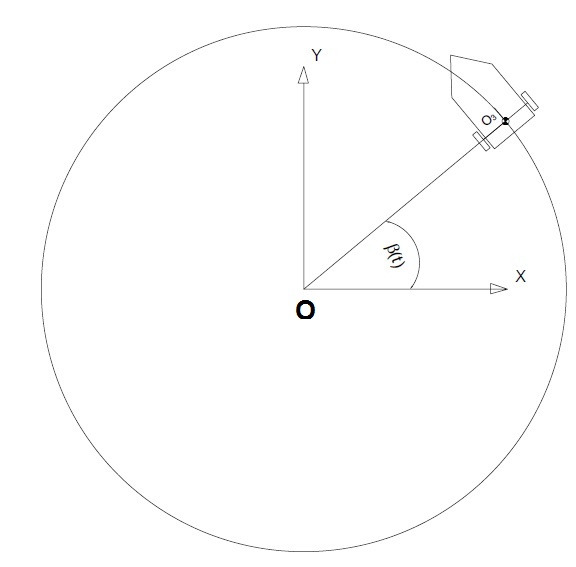
\includegraphics[height=250pt,keepaspectratio]{Chapter4/fig/pathCircle}
		\caption{Path traced by robot}
	\label{fig:CirTrace}
\end{figure}



\subsection{Inverse dynamics}
\label{sec:InvDynamics_NoSlip}
In order to find the torque required to trace the mobile platform on the circular curve given in Figure \ref{fig:CirTrace}, inverse dynamics was carried out.
Using the model's inverse kinematic,  the wheel velocity and acceleration were determined using pseudo inverse.  % from the equation given below. Where $r$ is radius of the wheel and $\theta_i$ is the wheel roll angle of wheel \#1 and \#2. The platform angular velocity is $\omega$ and the Cartesian velocity of point o3 is given by $\dot{x},\dot{y}$ in body coordinate system %   
The wheel angle, velocity and acceleration were used in the dynamics equation \ref{dnoc}  to calculate the torque required by each motor. The results are plotted in Figure \ref{fig:spiral}. 

The equation of  dynamic model  is given in equation \ref{dnoc}, where the actuated joints are  $\theta_a(t)=(\theta_l, \theta_r) $, the rear left and right wheel rotation angles. The dynamic  and kinematic  parameters used in the simulation is listed in table \ref{tb:massproperty}. The rear wheels $(i=1,2)$ and the platform $i=3$, twist $t_i^T=T_i\theta_a$, is given by Equations \ref{twist1}, \ref{twist2} and \ref{twist3}. The dynamic equation is of the vehicle on slope is given as 
\begin{equation}
\label{dnoc}
\begin{aligned}
T^TMT\ddot{\theta_a}&=-T^T(M\dot{T}+WMT)\dot{\theta_a}+T^T(w^J+w^G)\\
\text{where} \quad &
T=(T_1^T T_2^T T_3^T)^T, \quad M=diag(M_1, M_2, M_3)\\
T^TMT &=I_1+I_2+I_m+I_3= I_m+I_3\\
W&=diag(W_1,W_2,W_3),\quad w^G=g\sin\alpha, \quad \alpha=10^o
\end{aligned}
\end{equation}
where $w^G$, $ w^J$ and $\alpha$ represent the gravitational force acting along the inclined plane,  the external torque applied by a motor and the inclination of the plane to horizontal respectively. The generalized inertia matrix $I_m$ and $I_3$ are given in Equation \ref{eqn:I_wheel} and \ref{eqn:I_platform}.
As stated earlier the convective inertia term is zeros as the inertia matrices are constant. The expression for motor torque  is then given as 
\begin{equation}
T1^Tw_1^j=\tau_1, \quad T_2^Tw_2^j=\tau_2
\end{equation}
\begin{equation}
 T_3^Tw^g=\begin{pmatrix}
\rho\delta k & r(\lambda i+(1/2)j) \\
 -\rho\delta k & r(-\lambda i+(1/2)j)
\end{pmatrix}
\begin{pmatrix}
0\\
-jg\sin\alpha
\end{pmatrix}=\begin{pmatrix}
-\frac{1}{2}rg\sin\alpha\\ -\frac{1}{2}rg\sin\alpha
\end{pmatrix}
\end{equation} 

Figure \ref{fig:spiral} presents the torques required at the wheels of the vehicle while move up a spiral ramp  of slope $10^o$ and radius 5m. 

 \begin{figure}
	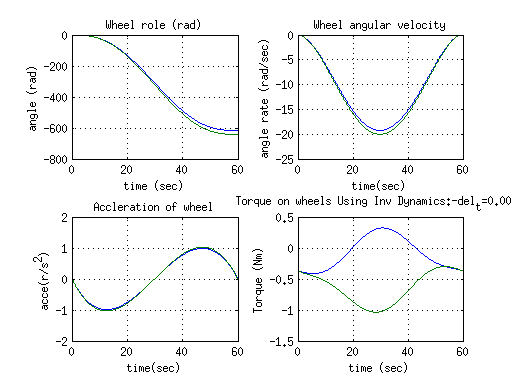
\includegraphics[height=300pt,keepaspectratio]{Chapter4/fig/FD}
	\captionof{figure}{Inverse dynamics of the mobile robot }
	\label{fig:spiral} 
\end{figure} 
%
\begin{table}[!htbp]
	\caption{Dynamic and kinematic parameters }
	\label{tb:massproperty}
	\centering
	\begin{tabular}{l l l}
		\hline
		\emph{Part Name}  & \emph{ Property} & \emph{Value} \\
		\hline
		Rear Wheels & & \\
		 $m_1,m_last section2$	& mass				&300g \\ 
		  $I_1,I_2$	& Moment of Inertia	& diag(242, 242, 465)kg $mm^2$\\
		Base Frame& & \\
		 $m_3$ & mass  & 70Kg \\
		 $ I_3$& Moment Of Inertia & $ \begin{pmatrix}
		 1.18& 0.01&-0.05\\ 0.01 & 1.28 & 0.08\\
		 -0.05 & 0.08 & 0.53
		 \end{pmatrix} Kg-m^2$ \\
		   l & length & 400mm\\
		  r & wheel radius (r) & 50mm\\
		 a & see Figure \ref{fig:CirTrace} & 220 mm \\ 
		\hline
		\end{tabular}
\end{table}



\section{Dynamics with Wheel Slip}
\begin{figure}
		\begin{minipage}[t]{0.5\textwidth}
		\centering
		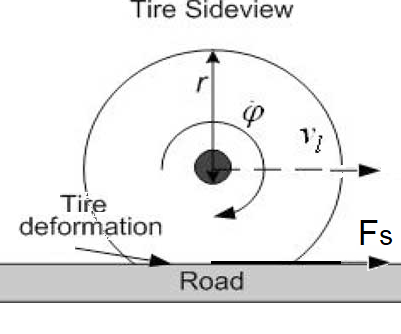
\includegraphics[width=2.5in]{Chapter3/fig/Slip} 
		\caption{Longitudinal slip \cite{wang2008modeling}}\label{fig:slip}
	\end{minipage}
	\hfill
	\begin{minipage}[t]{0.5\textwidth}
		\centering
		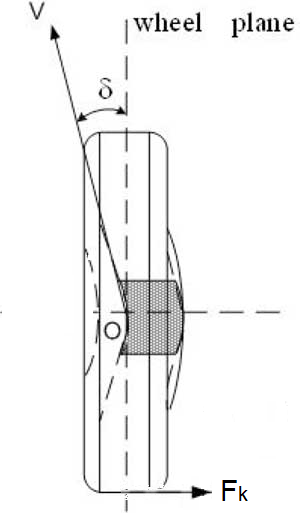
\includegraphics[width=1.5in]{Chapter3/fig/Skid} 
		\caption{Wheel Skid \cite{wang2008modeling}}\label{fig:skid}
	\end{minipage}
\end{figure}
The above section presented  the equations of motion  of a mobile robot  based on the no slip condition between the ground and the wheel, i.e. pure rolling condition. For RARS robot presented in this thesis the front steering wheels  are passive  but actively steered. Hence, the assumption of pure rolling condition of these wheels are no longer valid. Therefore, both the longitudinal slip and lateral slip (also called skid) are introduced in derive the equations of motion for RARS.
\subsection{Defining Slip}
\textbf{Longitudinal slip} occurs when the peripheral velocity of the wheel at the point of contact with respect to the ground, $\dot{\phi} r$ is different from the linear velocity $v_l$ of the wheel C.G., as shown in Figure \ref{fig:slip}, where, $\dot{\phi}$ is the angular rate of the wheel and $r$ is the effective radius of the wheel. Under pure rolling assumption  $\dot{\phi}  r=v_l$. However, this is not the case for a deformed wheel. The wheel slipping can be characterized by
slippage (or Slip ratio) \[\rho = \frac{\dot{\phi}  r - v_l}{\max(\dot{\phi}  r,v_l)}\] that has a  range of $ \rho \in [-1, 1]$. The case $\rho = 0$ indicates no wheel slippage whereas $\rho = 1$ implies a complete slippage, i.e., the wheel is not moving linearly despite its angular rotation. In normal road condition, the wheel's slippage $(\rho)$is usually in the range, $-1<\rho<1 $.
 The  longitudinal force ($F_s$) acting on the wheel due to slip is related to the slip ratio $\rho$. There are several adhesions models proposed that gives relation between the slip ratio and friction force at wheel-ground interface. One of the well known adhesion relations is the \textit{ magic formula} presented by Pacejka \cite{pacejka1992magic} which is used extensively in automotive industry to modeling tire forces. Other  friction models proposed in  literature  are by Claeys \cite{claeys2001dynamic}, Kulakowski \cite{kulakowski1991mathematical}  and Dugoff \cite{dugoff1970analysis}. 
 
 \textbf{Lateral slip }also called \textbf{skidding} is experienced when the wheel moves perpendicular to its plane. This is general encountered during cornering. This lateral movement is called skidding. The skidding produces frictional force perpendicular to the wheel plane as shown in Figure \ref{fig:skid} by $F_k$. The force $F_k$ is related to the slip angle $\delta$, which is the angle formed between the wheel plane and the velocity vector of the wheel, when projected on the ground plane.
 The force $F_k$ can again be found using magic formula \cite{pacejka1992magic} given in Equation \ref{eqn:magic} or any other adhesion model. Where instead of the slip ratio we use the slip angle as the independent parameter.
 
 %The magic formula \ref{eqn:magic} is reproduced below for completeness. In case of longitudinal slip $Y(x)$ represents longitudinal force $F_s$ and $x$ is the slip ratio $\rho$. For computation the lateral frictional  force $(F_k)$ due to skidding $x$ is replaced by the slip angle $\delta$. The constants $D$ represents the peak frictional force. The angle of  tangent at the origin is equal to $BCD$. $C$ controls the shape of the curve, $C=2.4$ for $F_k$ and  $C=1.65$ for $F_s$. $B$ controls the slope at origin. The remaining constant $E$ influences both the curvature of the curve near peak and also the position of $x_m$, where the peak is located.
 
 \begin{equation}\label{eqn:magic}
 Y(x)=D\sin[C \arctan{Bx -E(Bx-\arctan(bx))}]
 \end{equation}
%\begin{figure}
%	\centering
%	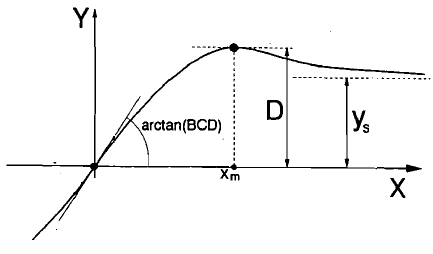
\includegraphics{Chapter3/fig/magicformula}
%	\caption{Tipical Curve of Magic Formula \cite{pacejka1992magic}}
%	\label{fig:magicformula}
%\end{figure}

\subsection{Kinematics with wheel slip}
\label{sec:slipKina}
 Figure \ref{fig:VehicleWithSlip}  shows the line digram of the RARS robot. Even though the actual RARS robot uses Davis linkage for steering the front wheels, here let us consider the steer angles $\psi_1$, $\psi_2$ corresponding to  each wheel. This makes the mathematical  modelling  more general. In order to simplify the model  link connecting the front wheels to the platform, tie rod, etc. associated with the steering mechanism   are excluded from the analysis, as their weights are small compared to the platform and wheels. The steering axis is assumed to pass through the center of the front wheel, i.e.,  the offset is zero.  It means $d_1=d_2=0$  ( Figure \ref{fig:gen}). Thus, $O_4=O_5$ and $O_6=O_7$. In Figure \ref{fig:VehicleWithSlip}  $O_4$  for wheel \#4 and $O_5$ for wheel \#5, denotes both the centre of the wheel and also the steering pivot point. The NoC approach was used to derive the equations of motion of the RARS robot with wheel slip taken into account for all the four wheels.
\begin{figure}
	\centering
	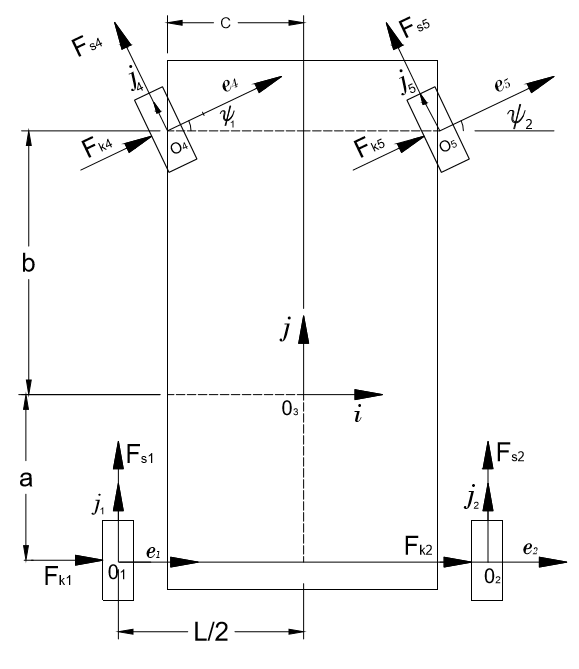
\includegraphics[width=\linewidth]{Chapter4/fig/VechileWithSlip}
	\caption{Free body diagram of RARS robot}
	\label{fig:VehicleWithSlip}
\end{figure}

The set of independent variables for this model is given by
\begin{equation}
\label{eqn:theta_slip}
\dot{\theta}=(\dot{\theta_1},\dot{\theta_2}, \dot{y_1},\dot{y_2},\dot{x},\dot{\psi_1},\dot{\psi_2},\dot{\theta_4},\dot{\theta_5})^T
\end{equation}
It may be noted that $\theta_i,\psi_i$  is same as defined earlier in Section \ref{sec:DynamicNoSlip}. The variables $\dot{y_1},\dot{y_2}$ are the linear velocity of centre of the rear wheels, i.e., of points point $O_1$ and $O_2$,, in the direction $j$ of the body coordinate system. The lateral slip of the rear wheels are denoted by $x_1$ and $x_2$ as shown in the Figure \ref{fig:VehicleWithSlip}. Due to rigidity constrains of the rear wheels there are related as follows
\[\dot{x_1}=\dot{x_2}=\dot{x}\] 
The velocities of points $O_1$ and $ O_2$ w.r.t the world coordinate ${X,Y,Z}$ and expressed in the robot's body co-ordinate system ${i,j,k}$ are given by 
\begin{equation}
\label{eqn:slip_do1}
\dot{o_1}=\dot{x}i +\dot{y_1}j, \quad \quad  \dot{o_2}=\dot{x}i +\dot{y_2}j
\end{equation}
Equating the velocity of point $O_3$ expressed in terms of $\dot o_1$ and $\dot o_2$, one gets
\begin{equation}
\label{eqn:slip_do3_rel}
\dot{o_3}=\dot{o_1}+\omega_3\times o_1o_3=\dot{o_2}+\omega_3\times o_2o_3
\end{equation}
Let $\omega_3$ be the angular velocity of platform, i.e., body \#3. Then 
\begin{equation}
	\label{eqn:slip_domega3}
	\omega_3=\bar{\omega_3}k, \quad \bar{\omega_3}=\frac{\dot{y_2}-\dot{y_1}}{l} 
\end{equation}
Using Equations \ref{eqn:slip_do3_rel} and \ref{eqn:slip_domega3} , we get
\begin{equation}
\label{eqn:slip_do3}
\dot{o_3}=(\dot{x}+\frac{a\dot{y_1}}{l}-\frac{a \dot{y_2}}{l})i+(\frac{\dot{y_1}}{2}+\frac{\dot{y_2}}{2})j
\end{equation}
The twist $t_3$ for body \#3 is obtained as
\begin{equation}
\label{eqn:slip_t3}
t_3=
\begin{pmatrix}
\omega_3\\
\dot{o_3}
\end{pmatrix}=T_3 \dot{\theta}, \quad \text{where,} \quad 
T_3=
\begin{pmatrix}
0 & 0& -k/l & k/l & 0 &0 & 0 &0 &0\\
0 & 0& ai/l+ j/2& -ai/l+j/2 & 0 &0 & 0 &0 &0\\ 
\end{pmatrix}
\end{equation}
or in expanded form
\begin{equation}
\label{eqn:slip_T3}
T_3=\left(
\begin{array}{ccccccccc}
0 & 0 & 0 & 0 & 0 & 0 & 0 & 0 & 0 \\
0 & 0 & 0 & 0 & 0 & 0 & 0 & 0 & 0 \\
0 & 0 & -\frac{1}{l} & \frac{1}{l} & 0 & 0 & 0 & 0 & 0 \\
0 & 0 & \frac{a}{l} & -\frac{a}{l} & 1 & 0 & 0 & 0 & 0 \\
0 & 0 & \frac{1}{2} & \frac{1}{2} & 0 & 0 & 0 & 0 & 0 \\
0 & 0 & 0 & 0 & 0 & 0 & 0 & 0 & 0
\end{array}
\right)
\end{equation}
Using the fact \[\frac{d i}{dt}=\bar{\omega_3}k\times i =\bar{\omega_3}j, \quad  \frac{d j}{dt}=\bar{\omega_3}k\times j =-\bar{\omega_3}i, \frac{d k}{dt}=\bar{\omega_3}k\times k =0 \] 
\begin{equation}
\label{eqn:slip_dT3}
\dot{T_3}=\begin{pmatrix}
0 & 0& 0 & 0 & 0 &0 & 0 &0 &0\\
0 & 0&-\frac{ \bar{\omega_3}}{2}i +\frac{a \bar{\omega_3}}{l}j& -\frac{ \bar{\omega_3}}{2}i -\frac{a \bar{\omega_3}}{l}j & 0 &0 & 0 &0 &0\\ 
\end{pmatrix}
\end{equation}

The angular velocities $\omega_1$ and $\omega_2$ of wheels \#1 and \#2 are given as
\begin{equation}
\label{eqn:slip_omega1and2}
\omega_1=\dot{\theta_1}i+\omega_3, \quad \omega_2=\dot{\theta_2}i+\omega_3
\end{equation}
Using Equations \ref{eqn:slip_do1} and \ref{eqn:slip_omega1and2}, one gets the twist vector for wheel \#1 as 
\begin{equation}
\label{eqn:slip_t1}
t_1=
\begin{pmatrix}
\omega_1\\
\dot{o_1}
\end{pmatrix}=T_1 \dot{\theta}
\end{equation} 
\begin{equation}
\label{eqn:slip_T1}
T_1=
\begin{pmatrix}
i & 0& -k/l & k/l & 0 &0 & 0 &0 &0\\
0 & 0& j& 0 & i &0 & 0 &0 &0\\ 
\end{pmatrix}=
\left(
\begin{array}{ccccccccc}
1 & 0 & 0 & 0 & 0 & 0 & 0 & 0 & 0 \\
0 & 0 & 0 & 0 & 0 & 0 & 0 & 0 & 0 \\
0 & 0 & -\frac{1}{l} & \frac{1}{l} & 0 & 0 & 0 & 0 & 0 \\
0 & 0 & 0 & 0 & 1 & 0 & 0 & 0 & 0 \\
0 & 0 & 1 & 0 & 0 & 0 & 0 & 0 & 0 \\
0 & 0 & 0 & 0 & 0 & 0 & 0 & 0 & 0
\end{array}
\right)
\end{equation}

and 
\begin{equation}
\label{eqn:slip_dT1}
\dot{T_1}=\begin{pmatrix}
\bar{\omega_3}j & 0& 0& 0 & 0 &0 & 0 &0 &0\\
0 & 0& -\bar{\omega_3}i& 0 & \bar{\omega_3}j &0 & 0 &0 &0\\ 
\end{pmatrix}
\end{equation}

Using Equations \ref{eqn:slip_do1} and \ref{eqn:slip_omega1and2} for wheel \#2 the twist vector $t_2$  is obtained as 
\begin{equation}
\label{eqn:slip_t2}
t_2=
\begin{pmatrix}
\omega_2\\
\dot{o_2}
\end{pmatrix}=T_2 \dot{\theta}
\end{equation} 
\begin{equation}
\label{eqn:slip_T2}
T_2=
\begin{pmatrix}
0 & i& -k/l & k/l & 0 &0 & 0 &0 &0\\
0 & 0& 0& j &i &0 & 0 &0 &0\\ 
\end{pmatrix}=
\left(
\begin{array}{ccccccccc}
0 & 1 & 0 & 0 & 0 & 0 & 0 & 0 & 0 \\
0 & 0 & 0 & 0 & 0 & 0 & 0 & 0 & 0 \\
0 & 0 & -\frac{1}{l} & \frac{1}{l} & 0 & 0 & 0 & 0 & 0 \\
0 & 0 & 0 & 0 & 1 & 0 & 0 & 0 & 0 \\
0 & 0 & 0 & 1 & 0 & 0 & 0 & 0 & 0 \\
0 & 0 & 0 & 0 & 0 & 0 & 0 & 0 & 0
\end{array}
\right)
\end{equation}

and 
\begin{equation}
\label{eqn:slip_dT2}
\dot{T_2}=\begin{pmatrix}
0 & \bar{\omega_3}j & 0& 0 & 0 &0 & 0 &0 &0\\
0 & 0& 0& -\bar{\omega_3}i & \bar{\omega_3}j &0 & 0 &0 &0\\ 
\end{pmatrix}
\end{equation}


Next,  the angular velocity of the steered wheel, i.e, body \#4, relative to the absolute frame is given as 
\[\omega_4=\dot{\theta_4}e_4+ \dot{\psi_1} k +\omega_3\]
The transformation matrix between the Frame $\{e_4,f_4\}$ attached to the wheel \#4 is given by the rotation matrix $R_4$. 
\begin{equation}
\label{eqn:slipR4}
R_4=\begin{pmatrix}
\cos \psi_1 & - \sin \psi_1\\
\sin \psi_1 & \cos\psi_1
\end{pmatrix}
\end{equation}
Then, $e_4= \cos\psi_1 i +\sin \psi_1 j$  and $\omega_4$ can be written as 
\[ \omega_4= \dot{\theta_4}( \cos\psi_1 i +\sin \psi_1 j)+ \dot{\phi_1} k +\omega_3 \]
Linear velocity of point $o_4$ is given by
\[ \dot{o_4}=\dot{o_3}+\omega_3 \times (-\frac{c}{2}i+bj) \]
or in terms of the twist as
\begin{equation}
\label{eqn:slip_t4}
t_4=
\begin{pmatrix}
\omega_4\\
\dot{o_4}
\end{pmatrix}=T_4 \dot{\theta}
\end{equation}
where 
\begin{equation}
\label{eqn:slip_T4}
T_4=\left(
\begin{array}{ccccccccc}
0 & 0 & 0 & 0 & 0 & 0 & 0 & \cos\psi_1 & 0 \\
0 & 0 & 0 & 0 & 0 & 0 & 0 & \sin\psi_1 & 0 \\
0 & 0 & -\frac{1}{l} & \frac{1}{l} & 0 & 1 & 0 & 0 & 0 \\
0 & 0 & \lambda_1 & -\lambda_1 & 1 & 0 & 0 & 0 & 0 \\
0 & 0 &\lambda_3 & \lambda_2 & 0 & 0 & 0 & 0 & 0 \\
0 & 0 & 0 & 0 & 0 & 0 & 0 & 0 & 0
\end{array}
\right)
\end{equation}
\begin{equation}
\label{eqn{:slip_dT4}}
\dot{T_4}=\begin{pmatrix}
0 & 0 & 0 & 0 & 0 & 0 & 0 & \lambda_4 & 0\\
0 & 0 & \lambda_7 & \lambda_6 & \bar{\omega_3}j & 0 & 0 & 0 & 0
\end{pmatrix}
\end{equation}

 \[\lambda_1=\frac{a+b}{l}, \quad \lambda_2=\frac{l-c}{2l}, \quad \lambda_3=\frac{l+c}{2l} \]
  \[\lambda_4=(\bar{\omega_3}+\dot{\psi_1}) (\cos\psi_1 j-\sin \psi_1 i) \]
  \[\lambda_6=-\bar{\omega_3}(\lambda_1 j+\lambda_2 i), \quad \lambda_7=\bar{\omega_3}(\lambda_1 j-\lambda_3 i)\]
Next, for wheel \#5  one gets 
\[\omega_5 = \dot{\theta_5} (R_5.e_5) + \dot{\psi_2} k + \omega_3 =
  \left(
\begin{array}{c}
\dot{\theta }_5 \cos \psi_2 \\
\dot{\theta_5} \sin \psi_2 \\
\dot{\psi_2}+\frac{-\dot{y_1}+\dot{y_2}}{L}
\end{array}
\right) \]
Accordingly, the linear velocity of point $o_5$ is given as 
\[ \dot{o_5}=\dot{o_3}+\omega_3 \times o_3o_5\]
where, \begin{equation}
\label{eqn:slipR5}
R_5=\begin{pmatrix}
\cos \psi_2 & - \sin \psi_2\\
\sin \psi_2 & \cos\psi_2
\end{pmatrix}
\end{equation}
Using  \[ o_3o_5=\frac{c}{2}i+bj\] along with $\omega_3$ and $\dot{o_3}$ from Equations \ref{eqn:slip_domega3} and  \ref{eqn:slip_do3},the following is obtained.
\[\dot{o_5}= \left( \dot{x}+\dot{y_1}(\lambda_1)-\dot{y_2}\lambda_1 \right)i +\left( \lambda_2\dot{y_1}+\lambda_3\dot{y_2}\right)j  \]
The twist of body \#5 , i.e., wheel \#5 is given as 
\begin{equation}
\label{eqn:slip_t5}
t_5=
\begin{pmatrix}
\omega_5\\
\dot{o_5}
\end{pmatrix}=T_5 \dot{\theta}
\end{equation}
Where
\begin{equation}
\label{eqn:slip_T5}
T_5=\left(
\begin{array}{ccccccccc}
0 & 0 & 0 & 0 & 0 & 0 & 0 & 0 & \cos \psi_2\\
0 & 0 & 0 & 0 & 0 & 0 & 0 & 0 & \sin\psi_2 \\
0 & 0 & -\frac{1}{l} & \frac{1}{l} & 0 & 0 & 1 & 0 & 0 \\
0 & 0 & \lambda_1 & -\lambda_1 & 1 & 0 & 0 & 0 & 0 \\
0 & 0 &\lambda_2& \lambda_3 & 0 & 0 & 0 & 0 & 0 \\
0 & 0 & 0 & 0 & 0 & 0 & 0 & 0 & 0
\end{array}
\right)
\end{equation}

Using the fact $\dot{e_5}=(\dot{\psi_2}+\bar{\omega_3})k\times e_5 =(\dot{\psi_2}+\bar{\omega_3})f_5$,  $f_5=-\sin \psi_2 i+\cos \psi_2 j$ and coordinate system $\{e_5,f_5\}$ is rotated by $\psi_2$ with respect to coordinate $ \{i,j\}$, $\dot{T_5}$ is given as

\begin{equation}
\label{eqn:slip_dT5}
\dot{T_5}=
\begin{pmatrix}
0 & 0 & 0 & 0 & 0 & 0 & 0 & 0 & \lambda_5\\
0 & 0 & \lambda_7 & \lambda_6 & \bar{\omega_3}j & 0 & 0 & 0 & 0
\end{pmatrix}
\end{equation}
where 
\[ \lambda_5 = (\bar{\omega_3}+\dot{\psi_2}) (\cos\psi_2 j-\sin \psi_2 i) \]
\subsection{Dynamics  with wheel slip}
\label{sec:slipDynamics}
The mass inertia matrix $M_i$ of the wheel and platform are same as that used in Section \ref{sec:GIM}. The generalized inertia matrix is then calculated using $T_i$ derived in Section  \ref{sec:slipKina}, as
\begin{equation}
I(\theta)=\sum_{i=1..n}(T_i^TM_iT_i)
\end{equation}
Where the inertial matrix $M_i$, for $ i=1,2,4,5$ given in Equation \ref{eqn:wheelInertiaMatrix} for each wheel. For platform  \[ I_p=\begin{pmatrix}
 p_{1,1} & p_{1,2} & p_{1,3}\\   
 p_{1,2} & p_{2,2} & p_{2,3}\\   
 p_{1,3} & p_{2,3} & p_{3,3}\\   
\end{pmatrix},  \quad  M_3=\begin{pmatrix}
 I_p & 0_{3x3}\\
 0_{3x3} & m_p 1_{3x3}
\end{pmatrix}\]
where $m_p$ is the mass of the platform and $1_{3x3}$ is the identity matrix.
The generalized inertia matrix $I$ is then given in terms of the  physical parameters of the wheel and platform as 
\begin{equation}
    I=
    \left(
\begin{array}{ccccccccc}
I_w & 0 & 0 & 0 & 0 & 0 & 0 & 0 & 0 \\
 0 & I_w & 0 & 0 & 0 & 0 & 0 & 0 & 0 \\
 0 & 0 & \bar{\alpha_1} & \bar{\alpha_2} & \bar \alpha_3  & -\frac{H}{l} & -\frac{H}{l} & 0 & 0 \\
 0 & 0 & \bar \alpha_2 & \bar \alpha_1 & -\bar\alpha_3 & \frac{H}{l} & \frac{H}{l} & 0 & 0 \\
 0 & 0 & \bar\alpha_3 & -\bar\alpha_3 & \bar\alpha_4& 0 & 0 & 0 & 0 \\
 0 & 0 & -\frac{H}{l} & \frac{H}{l} & 0 & H & 0 & 0 & 0 \\
 0 & 0 & -\frac{H}{l} & \frac{H}{l} & 0 & 0 & H & 0 & 0 \\
 0 & 0 & 0 & 0 & 0 & 0 & 0 & \bar \alpha_5 & 0 \\
 0 & 0 & 0 & 0 & 0 & 0 & 0 & 0 & \bar \alpha_6 \\
\end{array}
\right)
\end{equation}
where
\begin{equation*}
    \bar\alpha_1=\frac{p_{3,3}}{l^2}+m_p \left(\frac{a^2}{l^2}+\frac{1}{4}\right)+\frac{4 H}{l^2}+m_w \left(2 \lambda_1^2+\lambda_2^2+\lambda_3 ^2+1\right)
\end{equation*}
\[\bar \alpha_2=
-\frac{p_{3,3}}{l^2}+m_p \left(\frac{1}{4}-\frac{a^2}{l^2}\right)-\frac{4 H}{l^2}-2 m_w(\lambda_1^2 + \lambda_2 \lambda_3 )
\]
\[\bar\alpha_3=
\frac{a m_p}{l}+2 \lambda_1 m_w \]
\[\bar\alpha_4= m_P+4 m_w \]
\[\bar\alpha_5= I_w \cos^2{\psi_1}+H \sin^2{\psi_1}\]
\[\bar\alpha_6= I_w \cos^2{\psi_2}+H \sin^2{\psi_2}\]

The convective term $C(\theta,\dot{\theta})$ is calculated using the $T_i$, and $\dot{T_i}$ derived in Section \ref{sec:slipKina}, as
\begin{equation}
\label{eqn:RedConv}
C(\theta,\dot{\theta})=\sum_{i=1..n}T_i^T M_i\dot{T_i}+ \sum_{i=1..n}T_i^T W_i M_i T_i)\end{equation}
Introducing the following notions, the explicit expression of Equation \ref{eqn:RedConv}, is obtained below. 
\[ \delta_0=m_w\omega_3, \quad \delta_1= \frac{m_p \omega_3}{2}, \quad \delta_2=\frac{2a^2}{l^2}\delta_1+\frac{a \omega_3 p_{3,3}}{l^2}, \quad m_w\omega_3 \lambda_1(\lambda_2+\lambda_3)\]
\[ \delta_4 = \dot\theta_4 (H-I_w)\cos{\psi_1}\sin{\psi_1},\quad \delta_5=H\lambda_{4j}\sin{\phi_1}+I_w \lambda_{4i}\cos{\psi_1}-\frac{\dot \psi_1+\omega_3}{\dot\theta_4}\delta_4  \]
\[ \delta_6 = \dot\theta_5 (H-I_w)\cos{\psi_2}\sin{\psi_2},\quad \delta_7=H\lambda_{5j}\sin{\phi_2}+I_w \lambda_{5i}\cos{\psi_2}-\frac{\dot \psi_2+\omega_3}{\dot\theta_5}\delta_6  \]
\[\delta_8=\lambda _2 \delta _0+\lambda _3 \delta _0+\delta _0+\delta _1-\delta _2 \quad \delta_9=(\lambda _2+\lambda _3 +1)\delta _0  \]
\[ C=
\left(
\begin{array}{ccccccccc}
 0 & 0 & 0 & 0 & 0 & 0 & 0 & 0 & 0 \\
 0 & 0 & 0 & 0 & 0 & 0 & 0 & 0 & 0 \\
 0 & 0 & 0 & -\frac{a \delta _1}{l}-2 \delta _3+\frac{P_{33} \omega _3}{2 l} & \delta_8 & 0 & 0 & -\frac{\delta _4}{l}-\frac{\delta _6}{l} & 0 \\
 0 & 0 & 2 \delta _3 & \frac{P_{33} \omega _3}{2 l}-\frac{a \delta _1}{l} & \delta_8 & 0 & 0 & \frac{\delta _4}{l}+\frac{\delta _6}{l} & 0 \\
 0 & 0 & -\delta_9& -\lambda _3 \delta _0-\delta _0-\delta _1 & -\frac{2 a \delta _1}{l}-\delta _0 \lambda _2 & 0 & 0 & 0 & 0 \\
 0 & 0 & 0 & 0 & 0 & 0 & 0 & \delta _4 & 0 \\
 0 & 0 & 0 & 0 & 0 & 0 & 0 & \delta _6 & 0 \\
 0 & 0 & 0 & 0 & 0 & 0 & 0 & \delta _5 & 0 \\
 0 & 0 & 0 & 0 & 0 & 0 & 0 & 0 & \delta _7 \\
\end{array}
\right)\]
The wrench $\tau$ acting on the system is given as 
\begin{equation}
\label{eqn:slipTauSum}
\tau=\sum_{i=1..n}T_i^T w^w_i
\end{equation}
\begin{figure}
	\begin{minipage}[t]{0.5\textwidth}
		\centering
		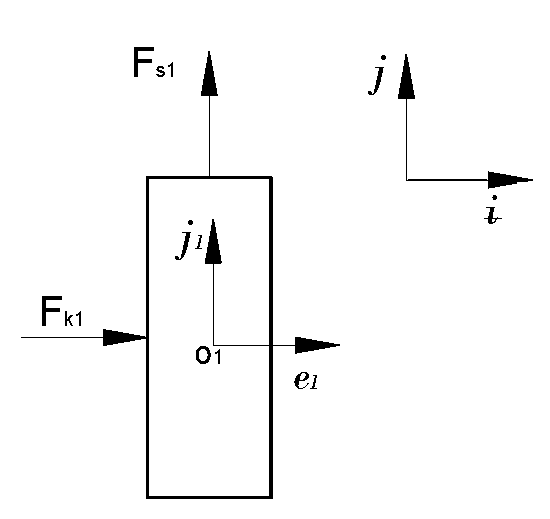
\includegraphics[width=0.8\textwidth]{Chapter4/fig/ForceWheel1}
		\caption{External force on rear wheel}\label{fig:ForceRearWheel}
	\end{minipage}
	\hfill
	\begin{minipage}[t]{0.5\textwidth}
		\centering
		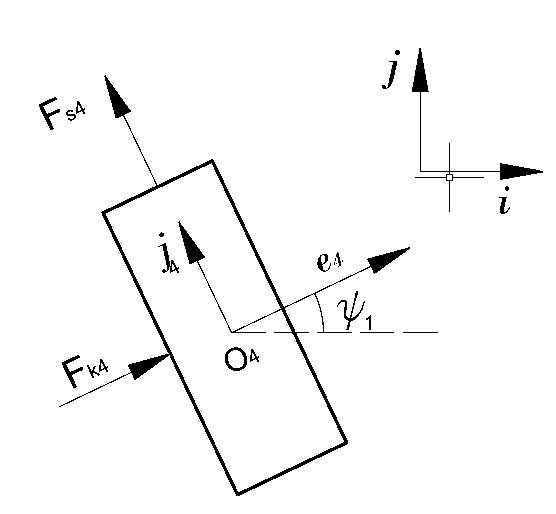
\includegraphics[width=0.8\textwidth]{Chapter4/fig/ForceWheel2}
		\caption{External forces on front wheel }\label{fig:ForceFrontWheel}
	\end{minipage}
	%\caption{Actuator effort}
\end{figure} 
The matrix $T_i$ has allready been calculated in the above section, whereas $w_i^w$ is derived next. The vector, $w_i^w$ is the working wrench acting on the individual bodies. This consists of all the external forces such as actuator force, friction force and gravitational force.
The forces acting on wheel 1, as shown in Figure \ref{fig:ForceRearWheel},  are the friction force due to longitudinal slip $Fs_1$ and frictional force  due to lateral slip or skidding, $Fk_1$ at the ground-wheel interface . The motor torque acting on the wheel 1 is $\tau_{m1}$.  Similarly forces acting on wheel 2 are $Fs_2$, $Fk_2$ and $\tau_{m2}$. Therefore, $w_1$ and $w_2$ are written as 
\begin{equation}
\label{eqn:wrenchWheelSlipRear}
 w_n=\begin{pmatrix}
\tau_{m,n}i\\
F_{k,n}i+F_{s,n}j
\end{pmatrix},  \quad n=\{1,2\}
\end{equation}
The superscript $w$ has been removed as it is understood that only working forces need to be considered in the formulation below. 
The front wheels have steering actuation, let the steering  torques be represented by $\tau_{s,4}$ and  $\tau_{s,5}$ for the wheel \#4, and \#5. The friction forces on the front steered wheel is shown in Figure \ref{fig:ForceFrontWheel} act along $\{e_4,f_4\}$ and $\{e_5,f_5\}$ for the two front wheels. No traction motor torque is applied to the front wheels as they are passive. Therefore, $w_4$ and $w_5$ are given by
\begin{equation}
\label{eqn:wrenchWheelSlipFront}
w_n=\begin{pmatrix}
\tau_{s,n}k\\
F_{k,n}e_n+F_{s,n}f_n
\end{pmatrix},  \quad n=\{4,5\}
\end{equation}
Since no external force is acting on the platform, i.e., body \#3, \[w_3=0_{6x1}\]

One can then calculate $T_i^Tw_i$, as

\begin{subequations}
	\label{eqn:slip_Tau_is}
	\begin{align}
	T_1^T w_1&=\begin{pmatrix}
	\tau_{m1} & 0 & F_{s1}& 0& F_{k1}&0&0&0&0
	\end{pmatrix} ^T\\
	T_2^T w_2&=\begin{pmatrix}
	0&\tau_{m2}& 0&F_{s2}&  F_{k2}&0&0&0&0
	\end{pmatrix} ^T\\
	T_3^T w_3&=0_{9x1} \quad \text{since } w_3=0\\
	T_4w_4&= \begin{pmatrix}
	0 & 0& \alpha_1& \alpha_2 & \alpha_3 &\tau_{s4}& 0&0 &0
	\end{pmatrix}^T\\
	T_5w_5&=\begin{pmatrix}
	0 & 0& \beta_1& \beta_2 & \beta_3 &0 &\tau_{s5}& 0&0
	\end{pmatrix}^T
	\end{align}
\end{subequations}
where 
\[\alpha_1=-\frac{\tau_{s4}}{l}+\lambda_1(F_{k4}C_{\phi_1}-F_{s4}S_{\phi_1})+\lambda_3(F_{k4}S_{\phi_1}+F_{s4}C_{\phi_1})\]
\[\alpha_2=\frac{\tau_{s4}}{l}-\lambda_1(F_{k4}C_{\phi_1}-F_{s4}S_{\phi_1})+\lambda_2(F_{k4}S_{\phi_1}+F_{s4}C_{\phi_1})\]
\[\alpha_3=(F_{k4}C_{\phi_1}-F_{s4}S_{\phi_1})\]
\[\beta_1=-\frac{\tau_{s5}}{l}+\lambda_1(F_{k5}C_{\phi_2}-F_{s5}S_{\phi_2})+\lambda_2(F_{k5}S_{\phi_2}+F_{s5}C_{\phi_2})\]
\[\beta_2=\frac{\tau_{s5}}{l}-\lambda_1(F_{k5}C_{\phi_2}-F_{s5}S_{\phi_2})+\lambda_3(F_{k5}S_{\phi_2}+F_{s5}C_{\phi_2})\]
\[\beta_3=(F_{k5}C_{\phi_2}-F_{s5}S_{\phi_2})\]
Therefore, the expression for  $\tau$ in  Equation \ref{eqn:slipTauSum} can be written as
\begin{multline}
\tau=(
\tau_{m1} \quad \tau_{m2} \quad (F_{s1}+\alpha_1+\beta_1) \quad( F_{s2}+\alpha_2+\beta_2) \\
 \quad  (F_{k1}+ F_{k2}+\alpha_3+\beta_3)\quad \tau_{s4}\quad  \tau_{s5} \quad 0 \quad 0 )  ^T
\end{multline}
The longitudinal  friction force $F_{si}$ for $i=1,2,4,5 $ is given by Equation \ref{eqn:magic} or any other adhesion model, with $ x $ as the slip ratio $\rho_i$ defined as
\[
x = \rho_i = \frac{\dot{\theta_i} r - \dot{o_i}.\hat{f_i}}{\max(\dot{\theta_i} r,\quad \dot{o_i}.\hat{f_i})}
\]
The lateral force  $F_{ki}$ for $i=1,2,4,5 $, i.e., the skid forces are given again by adhesion model such as Equation \ref{eqn:magic},  where $x$ is the slip angle $\delta$ defined in Figure \ref{fig:skid}. 
\[
x = \delta_i=\tan^{-1}(\frac{\dot{o_i}.e_i}{\dot{o_i}.f_i})
\]
It may be noted that $f_i,e_i$ are unit vectors of the coordinate system defined at each wheel centre and $\dot{o_i}$ are the velocities of wheel centres as shown in Figure  \ref{fig:ForceRearWheel}.
\subsection{Simulation}
To study the effect of wheel slip on the mobile robot dynamics, forward dynamics of the mobile robot was carried out. 
A reduced order  of the dynamic  equation derived in section \ref{sec:DynamicNoSlip} was used.
 The order was reduced by  neglecting the dynamic effect due to steering motion of the front wheels. The  variables $\psi_1$ and $\psi_2$ was  removed  from the  set of independent variables. They were directly set  at each time step using the relation,
 \[\phi_1=\arctan\left( \frac{(a+b)(\dot{y_2}-\dot{y_1})}{\dot{y_1}L}\right) , \quad
 \phi_2=\arctan\left( \frac{(a+b)(\dot{y_2}-\dot{y_1})}{\dot{y_2}L  }\right) 
 \]
  under the assumption $c=L/2$.
The total number of independent variables  was  reduced from  9 to 5. The new set of independent variables are now

\begin{equation}
\label{eqn:theta_slip_reduced}
\dot{\theta}_{red}=(\dot{\theta_1},\dot{\theta_2}, \dot{y_1},\dot{y_2},\dot{x})^T
\end{equation} 

The physical parameters used for the mobile robot are same as the one used in simulation of forward and inverse dynamics with ideal rolling condition for the wheels that  are listed in Table \ref{tb:massproperty}.
The generalized inertia  matrix $I_{red}$  and the convective term $ C_{red}$ of the reduced system are given by
\begin{equation}
I_{red}=\left(
\begin{array}{ccccc}
0.00046395 & 0 & 0 & 0 & 0 \\
0 & 0.00046395 & 0 & 0 & 0 \\
0 & 0 & 167.399 & -131.899 & 73.3333 \\
0 & 0 & -131.899 & 167.399 & -73.3333 \\
0 & 0 & 73.3333 & -73.3333 & 71.00
\end{array}
\right)
\end{equation}
\begin{equation}
C_{red}=\left(
\begin{array}{ccccc}
0 & 0 & 0 & 0 & 0 \\
0 & 0 & 0 & 0 & 0 \\
0 & 0 & 0 & -\frac{73.3333 (\dot{y_2} - \dot{y_1})}{l} & \frac{35.5 (\dot{y_2} - \dot{y_1})}{l} \\
0 & 0 & \frac{73.3333 (\dot{y_2} - \dot{y_1})}{l} & 0 & \frac{35.5 (\dot{y_2} - \dot{y_1})}{l} \\
0 & 0 & -\frac{35.5 (\dot{y_2} - \dot{y_1})}{l} & -\frac{35.5 (\dot{y_2} - \dot{y_1})}{l} & 0
\end{array}
\right)
\end{equation}
The equations of motion of the reduced system are given by 
\begin{equation}
I_{red}\ddot{\theta}_{red}+C_{red}\dot{\theta}_{red}=\tau_{red}
\end{equation}
The $\tau_{red}$ is calculated using Equation \ref{eqn:slipTauSum} with $i=1,2,3 $, where $w_i$ for $ i=1,2$ are given in Equation \ref{eqn:wrenchWheelSlipRear}.
Earlier $w_3=0$ was used as no external wrench was acting on it. In the reduced model case it is assumed that the frictional force acting on the front wheels are directly transmitted to the platform. Therefore, the moment acting about the C.G., of the platform, $O_3$ is given by
\begin{equation}
 	\label{eqn:redPlatMoment}
 	\tau_{p}=(F_{S4}+F_{K4}) \times (-i c+jb) +(F_{S5}+F_{K5}) \times (i c+jb) +T_s
\end{equation}
where $F_{Si},F_{Ki},\quad i=4,5$ are those explained in Section \ref{sec:slipDynamics}, $T_s$ is calculated as given  in Section \ref{sec:SteerinTorqueStatic}.
Therefore, $w_3$ is written as 
\begin{equation}
w_3=\begin{pmatrix}
\tau_{p}\\
F_{S4}+F_{K4}+F_{S5}+F_{K5}
\end{pmatrix}
\end{equation}

To evaluate $F_{s,i} $ and $F_{k,i}$ for $i=1,2,4,5$,   which are function of  slip ratio or slip angle,  Equation \ref{eqn:friction_Slip}  \cite{balakrishna1995modeling}, which is based on adhesion model proposed by \cite{dugoff1970analysis} was used.  A representative Friction-slip curve with the peak friction co-efficient, $\mu_{peak}=0.1$, is given in  Figure \ref{fig:friction_Slip}. The longitudinal and lateral friction forces acting on the wheels are given as $Fs=\mu N_i$ where $N_i$ is the normal force action on the wheel due to ground reaction.  
\begin{equation}
\label{eqn:friction_Slip}
\mu =
\begin{cases}
-(\lambda-0.15)\frac{0.34\mu_{peak}}{0.85}-\mu_{peak}, & -0.15\le\lambda \le -1.00,\\
(\lambda-0.15)\frac{\mu_{peak}}{0.15}+\mu_{peak}, & -0.15<\lambda<0.15,
\\
-(\lambda-0.15)\frac{0.34\mu_{peak}}{0.85}+\mu_{peak}, & 0.15\le\lambda \le 1.00,
eqn
\end{cases}
\end{equation}
To calculate $F_{Si},F_{Ki}$ for $ i=4,5$ spin rate of front wheels $\dot\theta_4,\dot\theta_5$ are required. This is obtained from Equation \ref{eqn:simpDynFront} which represents the dynamics  of the front wheels, where $r$ is the radius of wheel and $I_w$ is the inertia of wheel about $e_i$.
\begin{equation}
\label{eqn:simpDynFront}
I_w\begin{pmatrix}
 \ddot\theta_4\\
 \ddot\theta_5
\end{pmatrix}
=
\begin{pmatrix}
F_{s4} r\\
F_{s5} r
\end{pmatrix}
\end{equation}
 Figure \ref{fig:InputTorqueProfile} shows input torque applied to the two rear wheels for the forward dynamic simulation. This torque profile for the pair of rear wheels was generated by inverse dynamics  of the mobile robot presented in Section \ref{sec:InvDynamics_NoSlip} to trace a circular path given in Figure \ref{fig:CirTrace} and represented by Equation \ref{path} on a flat surface under the assumption of pure rolling condition of all wheels. 

\begin{figure}
	\begin{minipage}[t]{0.5\textwidth}
		\centering
		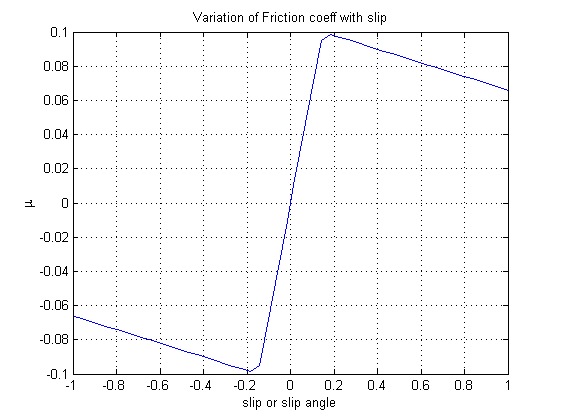
\includegraphics[width=\textwidth]{Chapter4/fig/frictionVsSlip}
		\caption{Friction model}\label{fig:friction_Slip}
	\end{minipage}
	\hfill
	\begin{minipage}[t]{0.5\textwidth}
		\centering
		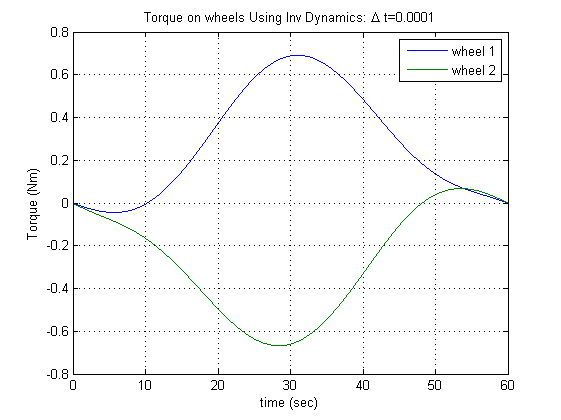
\includegraphics[width=\textwidth]{Chapter4/fig/InputTorqueProfile}
		\caption{Input Torque Profile }\label{fig:InputTorqueProfile}
	\end{minipage}
	%\caption{Actuator effort}
\end{figure}
\ 
\subsection{Results and inference}
The path traced by the RARS mobile robot  with  $\mu_{peak} =0.3$ is shown in Figure \ref{fig:pathWithMu3}. There is no visible difference between the  actual path traced  and the given path in terms of lateral shift. Circular path radius is same for both curves, though the vehicle is not able to complete the path. The path ends at ${(4.862,-1.166)}$ denoted as ``End Point" in  Figure \ref{fig:pathWithMu3} instead of  ${(5,0)}$. This deviation is assumed to be there due to the longitudinal slip at the wheel-surface interface.  Figure \ref{fig:ForcesMu3} presents the plot of lateral force acting on the vehicle during the period of its motion. The centrifugal force, denoted by green line,  tries to shift the vehicle laterally is below the maximum frictional resistance provided by the wheel-surface interface, denoted by the red line. Hence, the net lateral force acting on the mobile robot at any point of time during the motion is zero as indicated by the blue line.

When the friction coefficient is reduced to  $\mu_{peak} =0.1$, both lateral and longitudinal shift are present, as shown in Figure \ref{fig:pathWithMu1}. The  net lateral force acting on the vehicle, i.e., the blue curve of Figure \ref{fig:ForcesMu1} is greater than zero between 20 sec to 40 sec. This lateral force is responsible for the deviation of the actual path traced from the given path. The deviation increases from point ``A" to point ``B" in Figure \ref{fig:pathWithMu1}. This is region of the path where the centrifugal force exceeds the frictional force. After point ``B" the curve maintains constant radius as the net lateral force acting on the mobile robot again becomes zero. 

Note that Figure \ref{fig:beta1} shows the variation of $\beta(t)$ defined in Equation \ref{path} and $\dot\beta(t)$ with time.  Figure \ref{fig:ForcesMu1} indicates  that lateral slip initiates for $\mu=0.1$ at time $t=18.3s$. This corresponds to angular velocity of $ \dot \beta =0.1412 $ rad/sec as can be read from Figure \ref{fig:beta1} at time $t=18.3s$.
\begin{figure}
	\centering
	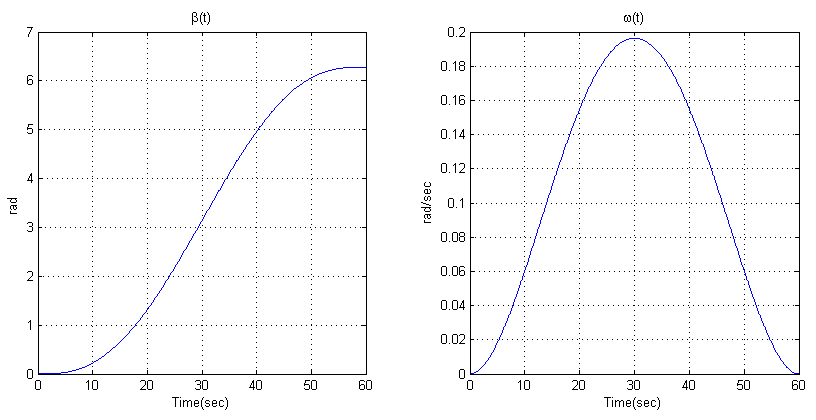
\includegraphics[width=\linewidth]{Chapter4/fig/beta}
	\caption{Plot of $\beta$ and $\dot{\beta}$}
	\label{fig:beta1}
\end{figure}
The linear velocity of the robot to initiate lateral slipping is given by $R\dot{\beta}$, which is equal to $0.7$  m/sec. The robot at hand is restricted to the speed of $0.5$ m/sec as specified in the robot specification in Table \ref{tb:specifications}. The estimated coefficient of friction between the Polyurethane wheel liner and factory floor is around $0.3$. Therefore skidding of the mobile robot RARS is unlikely during teleoperation. 
\begin{figure}
	\begin{minipage}[t]{0.5\textwidth}
		\centering
		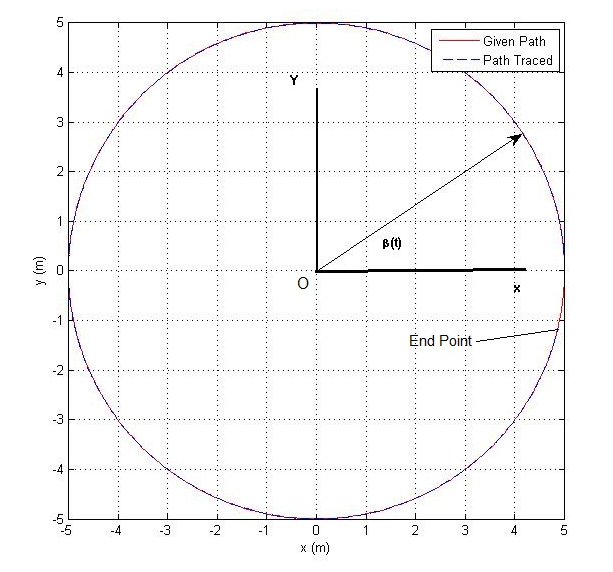
\includegraphics[height=3in]{Chapter4/fig/PathWithMu-3slip}
		\caption{RARS path traced when $\mu=0.3$}\label{fig:pathWithMu3}
	\end{minipage}
	\hfill
	\begin{minipage}[t]{0.5\textwidth}
		\centering
		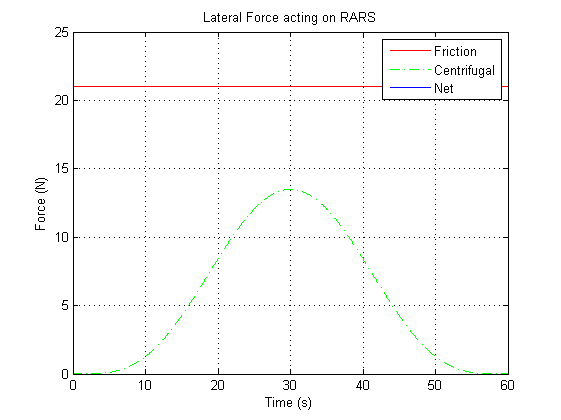
\includegraphics[height=3in,width=\textwidth]{Chapter4/fig/ForceMu-3}
		\caption{Forces on RARS when $\mu=0.3$ }\label{fig:ForcesMu3}
	\end{minipage}
	%\caption{Actuator effort}
\end{figure}
\begin{figure}
	\begin{minipage}[t]{0.5\textwidth}
		\centering
		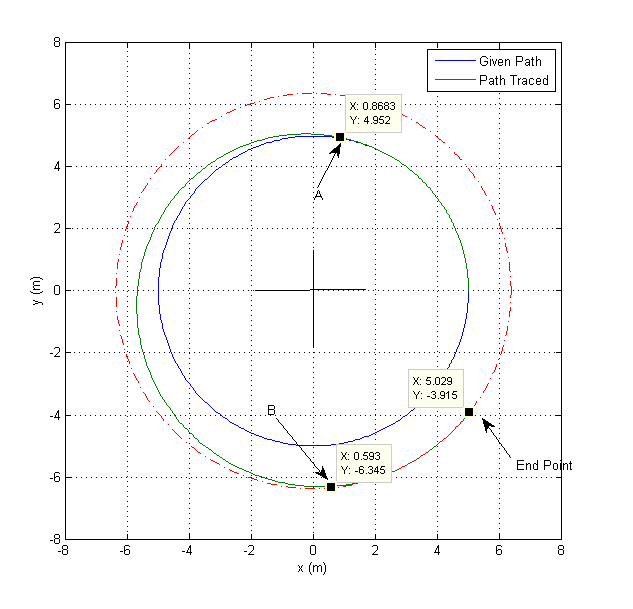
\includegraphics[height=3in]{Chapter4/fig/PathWithMu-1slip}
		\caption{RARS path traced when $\mu=0.1$}\label{fig:pathWithMu1}
	\end{minipage}
	\hfill
	\begin{minipage}[t]{0.5\textwidth}
		\centering
		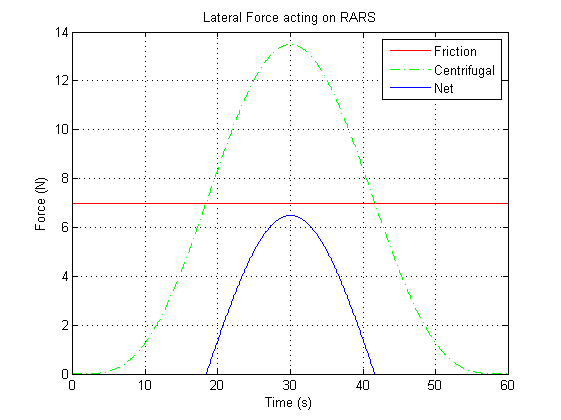
\includegraphics[height=3in,width=\textwidth]{Chapter4/fig/ForceMu-1}
		\caption{Forces on RARS when $\mu=0.1$ }\label{fig:ForcesMu1}
	\end{minipage}
	%\caption{Actuator effort}
\end{figure}
\section{Dynamical Model of Steering System}
Typically, the tuning of steering motor is done while the vehicle is stationary. Hence, an independent dynamic model for steering system is essential, which is carried out in this section. 
The  steering system is shown in Figure \ref{fig:SteerAsm}. The equations of motion were derived under the assumptions,  that the vehicle body \#3 was at rest and  the mass of links \#8 and \#9 were negligible compared to other links. The kinematic energy of each body except \#8 and \#9 is derived below.

The kinetic energy of link  \#6 is given by
\begin{equation}
 K_6=\frac{1}{2}(m_6((x^b_6)^2+(y^b_6)^2)+I_{6zz})\dot{\phi_6}
\end{equation}
 where, $m_6$ is the mass, $(x^b_6,y^b_6)$  the coordinate of c.m.  expressed  in the body co-ordinate frame $B:\{i_6,j_6,k_6\}$ as shown in Figure \ref{fig:SteerLink} and $I_{6zz}$ is the moment of inertia in the body coordinate of link \#6.
 
 
 Next we derive the kinetic energy of body \# 4, the wheel. 
 The coordinate of c.g of wheel, $O_4$ in the world  $F:\{i,j,k\}$  is given by \[ \begin{pmatrix}
x_{4}\\y_{4} \end{pmatrix}_F
= \begin{pmatrix}-\frac{l}{2} \\0
\end{pmatrix}+
\begin{pmatrix}
		\cos\phi_6 &  -\sin\phi_6\\ -\sin\phi_6 & \cos\phi_6
\end{pmatrix} + 
\begin{pmatrix}
			-l_3\\0
\end{pmatrix}\]
\begin{figure}
	\begin{minipage}[t]{0.5\textwidth}
		\centering
		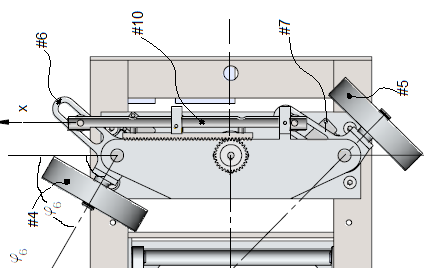
\includegraphics[width=3in]{Chapter4/fig/SteerModel} 
		\caption{Steering assembly}\label{fig:SteerAsm}
	\end{minipage}
	\hfill
	\begin{minipage}[t]{0.5\textwidth}
		\centering
		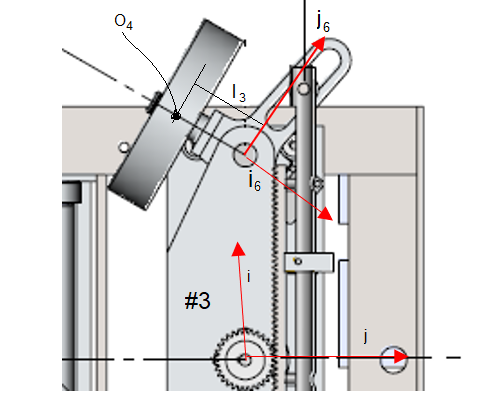
\includegraphics[width=2in]{Chapter4/fig/link} 
		\caption{Steering linkage }\label{fig:SteerLink}
	\end{minipage}
	%\caption{Actuator effort}
\end{figure}
 	
  The linear velocity $\dot{O}_4$  and its angular velocity $\omega_6$  expressed in the world frame $F:\{i,j,k\}$ is given by
 \begin{eqnarray}
 \dot{O}_4=l_6\dot{\phi_6}[\sin\phi_6, ~ -\cos\phi_6] ^T
 \end{eqnarray}
 
 \begin{equation}
 \omega_6=\dot\phi_6k_6+\dot\theta_4i_6 ~=~ [\dot\theta_4\cos\phi_6,~ \dot\theta_4\sin\phi_6,~ \dot\phi_6]^T
 \end{equation} where, $l_6$ is the length as shown in Figure \ref{fig:SteerLink}  and $\dot\theta_4$ is the spinning rate of the wheel about axis $i_6$.
 Then the kinetic energy of body \#4 is given by
\begin{equation}
 K_4=\frac{1}{2}(m\dot O_4 ^T ~\dot O_4+ \omega_6^T [I_6]_F~\omega_6  )
 \end{equation}
 \begin{multline}
 K_4=\frac{1}{2} l_6^2 \dot\phi_6 m \begin{pmatrix}
 \sin\phi_6, ~ -\cos\phi_6
 \end{pmatrix}
 \begin{pmatrix}
 \sin\phi_6\\ -\cos\phi_6
 \end{pmatrix}\\
 + 
 \begin{pmatrix}
 \dot\theta_4 \cos\phi_6, ~ \dot\theta_4 \sin\phi_6, ~\dot\phi_6
 \end{pmatrix}[I_6]_F
 \begin{pmatrix}
 \dot\theta_4 \cos\phi_6\\ \dot\theta_4 \sin\phi_6\\ \dot\phi_6
 \end{pmatrix}
 \end{multline} Where $[I_6]_F$ is the inertia matrix of wheel about its c.g. expressed in world frame $F$.
 In general the moment of inertia matrix of the body is known in the body frame $B$, ie $[I_6]_B$. This can be transformed to the world coordinate frame $F$ by using the formula
 \[ [I_4]_F=R^F_B[I_4]_B [R^F_B]^T\] where, $R^F_B$ represents rotation transformation matrix between the fixed Frame, $F$, and the body frame, $B$. 
 The above Equation, after above transformation can be written as
 \begin{equation}
 K_4=\frac{1}{2}(l_3^2\dot\phi_6^2m_4+[I_{4xx}]_B\theta_4^2)
 \end{equation} 
where, $I_{4zz} $ is the moment of inertia of the wheel about its z axis in the body coordinate frame.

The kinetic energy of the tie rod, i.e., body \#10, which under goes linear reciprocating motion in a plane is given by
\begin{equation}
K_{10}=\half m_{10} \dot{x}
\end{equation} where, $x$ is the displacement of the tie rod and $m_{10}$ is its mass.


The kinetic energy of body \#5, i.e., second wheel and second link \#7 can be derived in a similar fashion as that of body \#4 and \#6 respectively. The kinetic energy of body \#7 is given as
\begin{equation}
K_7=\frac{1}{2}(m_7((x^b_7)^2+(y^b_7)^2)+I_{7zz})\dot{\phi_7}
\end{equation}
where, $m_7$ is the mass and  $I_{7xx}$ moment of inertia of body \#7 .

The kinetic energy of body \#5  is given as
 \begin{equation}
K_4=\frac{1}{2}(l_3^2\dot\phi_7^2m_5+[I_{5xx}]_B\theta_5^2)
\end{equation} 
 where $m_5$  is the mass and $I_{5xx}$ moment of inertia of body \#5.
 

From the geometry of Figure \ref{fig:davis} following relations can be derived 
\begin{equation}
\label{eqn:thetaTox}
\tan(\alpha-\phi_6)=\frac{b+x}{h}, \quad \quad \tan(\alpha-\phi_7)=\frac{b-x}{h}
\end{equation}
\begin{equation}
\label{ro}
x^b_6+y^b_6=x^b_7+y^b_7=r_0
\end{equation}
\begin{equation}
\dot{\phi_6}=\dfrac{h\dot x}{h^2+b^2+2bx+x^2}=f_1(x)\dot x,\quad \dot{\phi_7}=\dfrac{h\dot x}{h^2+b^2-2bx+x^2}=f_2(x)\dot x
\end{equation}
 Therefore the total kinetic energy of steering unit is 
\[K_s=\sum_{i=4..10}K_i\]
using the expression for $K_i$  and using Equations 4.48, 4.49 and 4.50, the above equation for $K_s$  is written as 
\begin{multline}
	K_s=\frac{\dot x^2}{2} \left( m_{10}+(m_l r^2_0+I{zz})+l^2_3m_w \right) \left(f^2_1(x)+f^2_2(x) \right)\\ + \half I_{wxx}\left(\dot\theta^2_4  +\dot\theta^2_5\right)
\end{multline}
under the following assumptions \[l_3=l_4, \quad m_4=m_5=m_w, \quad m_6=m_7=m_l, \quad I_{7zz}=I_{6zz}=I_{zz}\]
The Lagrangian in this case is simply the kinetic energy, i.e,  $L=K_s$. Since the external forces acts only along the $x$ ordinate, via steering motor. We get
\[F_x= \dfrac{\partial}{\partial t}\dfrac{\partial L}{\partial \dot x} - \dfrac{\partial L}{\partial x}\]
or 
\begin{multline}
\label{eqn:SteerDyn}
F_x=\ddot{x}\left[ m_{10}+\left(m_lr_o^2+I{zz}+l^2_3m_w \right) \right] \left( f_1^2+f_2^2 \right)\\
+2\dot x^2 \left(m_lr^2+I{zz}+l_3^2 m_w \right) \left( f_1 \dot f_1 +f_2 \dot f_2\right)+F_1+F_2
\end{multline}
The external force $F_1$ and $F_2$ in the above equation is given by
\[F_i=\dfrac{T_s}{h},i={1,2} \]
where $T_s$ is evaluated using Equation \ref{eqn:brake} assuming symmetric loading of both the wheels. The derivative of $f_1(x)$ and  $f_2(x)$ is given by 
\[ \dfrac{df_1}{dt}=-\dfrac{2(x+b)h}{(h^2+b^2+2bx+x^2)^2}, \quad \dfrac{df_2}{dt}=-\dfrac{2(x-b)h}{(h^2+b^2-2bx+x^2)^2}\]



\subsection{Design of PID controller}
To control the steer angle of the front wheels a computed torque controller \cite{craig2005introduction} was designed. If $U$ denotes the auxiliary control input then $F_x$ is given by
\begin{multline}
\label{eqn:SteerCont}
F_x=U\left[ m_{10}+\left(mr_o^2+I{zz}+l^2_3m_w \right) \right] \left( f_1^2+f_2^2 \right)\\
+2\dot x^2 \left(mr^2+I{zz}+l_3^2 m_w \right) \left( f_1 \dot f_1 +f_2 \dot f_2\right) 
+F_1+F_2
\end{multline}
eliminating  $F_x$ using Equation \ref{eqn:SteerDyn} and Equation\ref{eqn:SteerCont}, we get
\begin{equation}
\label{eqn:SteerCont2}
\ddot x =U
\end{equation}
If $x_d$, is the set point for the displacement of the rack of the steering system and $e(t)=(x(t)-x_d)$ is the position error, we define auxiliary input $U$ as  
\begin{equation}
\label{eqn:SteerCont3}
 U=-K_d \dot x -K_p \left(x(t)-x_d \right) -K_i\int e(t)dt \end{equation}
then Equation \ref{eqn:SteerCont2} which represents the overall dynamics of the steering mechanism along with the controller, can  be written as 
\[\ddot e(t) +K_d \dot{e}(t) +K_p e(t)+ K_i\int e(t)dt=0 \]
It is be noted that $\dot e(t)=\dot x$ and $\ddot e(t)=\ddot x$, since $x_d=const$. Given that  $y_1(t)= \int e(t)$ and $Y=[y_1,~y_2,~y_3]^T$, the above equation can be rewritten in state space \[\dot{Y}=AY\] or
\begin{equation}
\begin{pmatrix}
\dot y_1 \\ \dot y_2 \\\dot y_3
\end{pmatrix}
=
\begin{pmatrix}
0 & 1 & 0\\ 0 & 0 & 1\\ -K_i & -K_d & -K_p
\end{pmatrix}
\begin{pmatrix}
 y_1 \\ y_2 \\ y_3
\end{pmatrix}
\end{equation}
With $K_d=20,~K_p=60,~K_i=100 $ the system is stable as  the state transition matrix $A$ has all its eigen values, $\lambda$, with negative real part, as given below 
\[ \lambda= \{-16.7794 + 0.0000i, ~ -1.6103 + 1.8348i, ~ -1..6103 - 1.8348i\}\]
 These controller parameters were arrived by trial and error using multiple simulation. The guiding principle behind the selection of these parameters was to choose one root far away form the imaginary axis so that its contribution to the response decays faster with the respect to  the other two roots.  The system then behaves as second order system. The remaining two roots thus governs the dynamics of the system.  They were chosen as complex conjugate with negative real part near the imaginary axis so as to make the steering unit dynamics  under damped.

\subsection{Simulation and results}
The simulation of the  dynamic Equation \ref{eqn:SteerDyn} and controller given by Equations \ref{eqn:SteerCont} and \ref{eqn:SteerCont3} was carried out with the step change in steering angle responding to $ 20~mm$  rack displacemet $(x)$.  The parameter used for the nominal plant were obtained form solid model of the parts and are listed in table \ref{tb:steerPara}. The results of the wheel orientations and the actuator effort required are given in Figure \ref{fig:SteerPos} and \ref{fig:SteerEfort} respectively.

\begin{table}[!htbp]
	\caption{Key parameters steering assembly.}
	\label{tb:steerPara}
	\centering
	\begin{tabular}{l l l }
		\hline
		
		%\emph{Parameter}  & \emph{Example} & \emph{Font size and style} \\
		%\hline
		Wheel Mass& $m_w $ &$ 350~g$  \\ 
		Wheel Inertia & $I_{wxx}$ & $463~ Kg ~mm^2$\\
		Connecting Rod Mass & $m_{10} $& $200~g$ \\
		Link mass& $m_l$ & 80g\\
		Link Inertia & $I_{zz} $& $60834~Kg ~mm^2$\\
		Link Cg distance & $r_o$ & $18mm$\\
		\hline
	\end{tabular}
\end{table}

 
\begin{figure}
	\begin{minipage}[t]{0.5\textwidth}
		\centering
		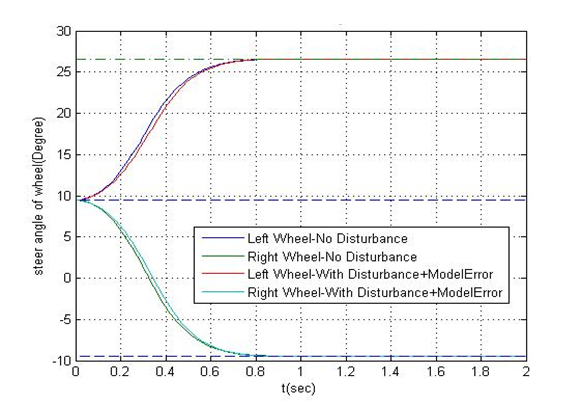
\includegraphics[width=3in]{Chapter4/fig/SteeringPos} 
		\caption{Change in steer angle}\label{fig:SteerPos}
	\end{minipage}
	\hfill
	\begin{minipage}[t]{0.5\textwidth}
		\centering
		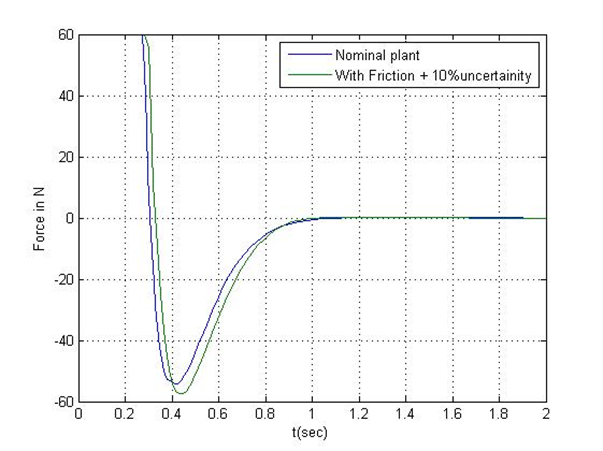
\includegraphics[width=3in]{Chapter4/fig/SteerEffort} 
		\caption{Control effort}\label{fig:SteerEfort}
	\end{minipage}
	%\caption{Actuator effort}
\end{figure} 
The simulation results establishes that with $10\%$ error in plant parameters there is practically no deviation in the performance of the controller. The results also predicts a settling time of $0.8~sec$ for the system. It may be noted that the roll velocity of the wheel does not affect the dynamics of the steering system as is indicated by the absence of $\dot\theta_4$ and $\dot\theta_5$  from Equation \ref{eqn:SteerDyn} .
\section{Summary}
In this chapter, the dynamic equations were derived for  the most general form of passive wheel configuration. Even though  only two passive wheel configuration was considered the same formulation can be extended to any number of  wheels. It is shown that the  dynamics of standard caster wheels is a special case of the  general case with $d_1=0$. It is also proven why a caster needs  non-zero caster offset. There is a  need of extra actuator in case $d_2=0$. 

NOC based approach to model wheel slip in dynamics of a mobile manipulator was presented in this chapter. RARS  being a redundantly actuated system has a inherent tendency to induce slip in the wheels if their velocities and orientations are not synchronised. A simulation study of RARS was carried out to assess the effect of  wheel slip on its dynamics. 

The steering mechanism was modelled separately. Simulation was used to find the   controller parameters which makes the system marginally damped. This ensured that there is no over steering while keeping the settling time small. These controller parameters were later used to tune the actual system.   
    






\cleardoublepage
\chapter{Control of a Mobile Manipulator }
\label{c5_Control}
In this chapter, the control architecture of the tele-operated  mobile manipulator or platform  is presented. The user interface for teleoperation is discussed. The control algorithm  running on the mobile manipulator and the hardware used for the control of traction and steering is discussed. The protocol used  for communication between the robot and the user interface is also described in detail.
\section{Control Architecture and Hardware}


\begin{figure}
	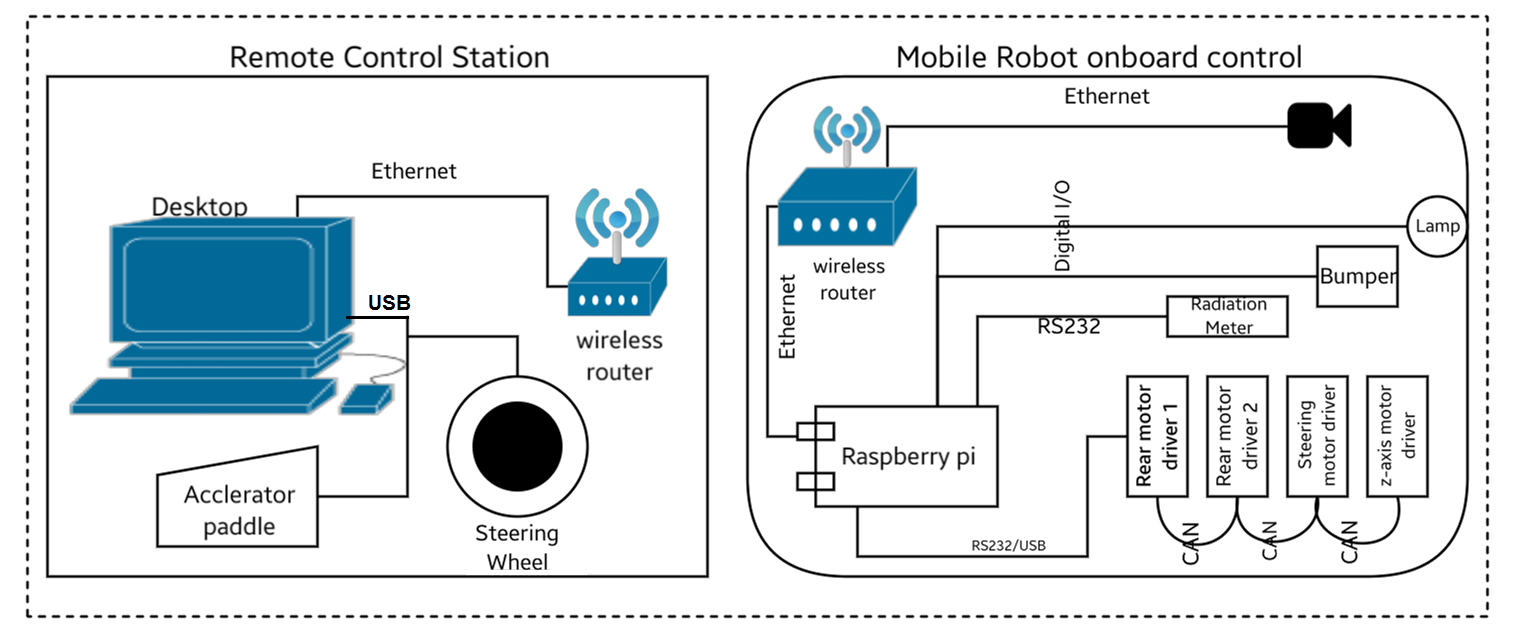
\includegraphics[width=\linewidth,keepaspectratio]{Chapter3/fig/controlblock}
	\captionof{figure}{Control architecture }
	\label{fig:ControlBlockDiag} 
\end{figure} 
The mobile manipulator explained in chapter \ref{ch_3:Design} was planned to be teleoperated over a wireless network. The control block diagram and architecture are shown in Figure \ref{fig:ControlBlockDiag}. It has a remote control station which is the interface for the operator and a local onboard controller of the mobile robot. They  communicate over a dedicated wireless network. The remote station sends data packet in every  50 milliseconds (20Hz) to the mobile robot. The commanded velocity, steer angle,  z position of the platform, and  state of the detector and headlamps constitute the data packet sent by the remote station, as shown in Figure \ref{fig:sentBytes}. The onboard controller of the mobile robot replies with a data packet consisting of the $X$, $Y$ position and orientation $\theta$ of the robot, the current steer angle, angular velocities of each wheel, the z position of the top platform,  battery voltage  and current of each motor. They are indicated in Figure \ref{fig:recvBytes}.
\begin{figure}
	
	\begin{minipage}[t]{0.5\textwidth}
		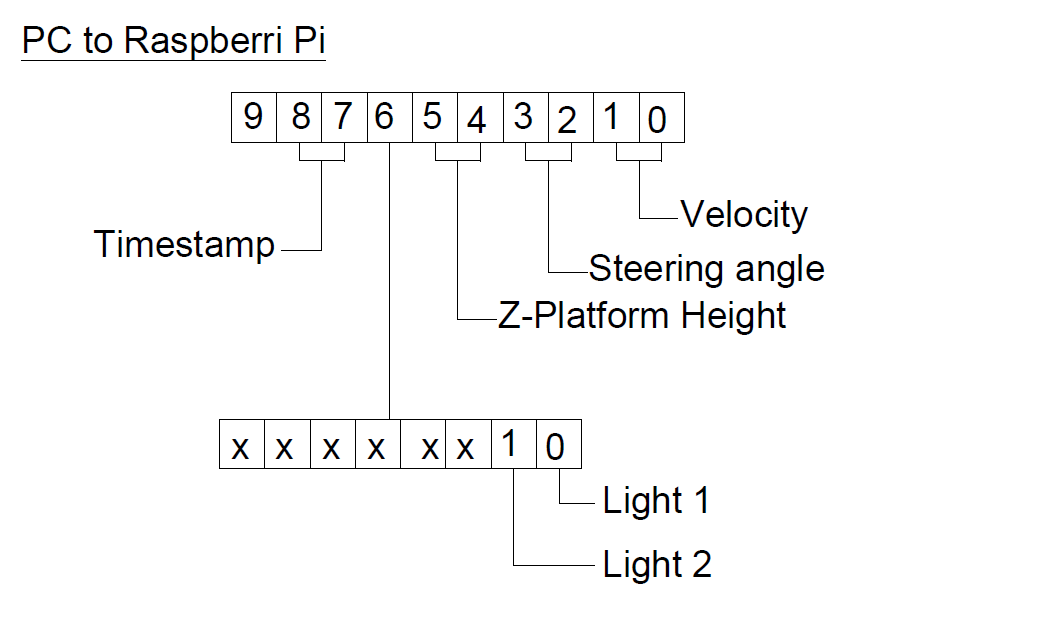
\includegraphics[width=\linewidth,keepaspectratio]{Chapter5/fig/bitconfig}
		\captionof{figure}{Data from PC to the robot }
		\label{fig:sentBytes} 
	\end{minipage}
\hfill
   \begin{minipage}[t]{0.5\textwidth}
   		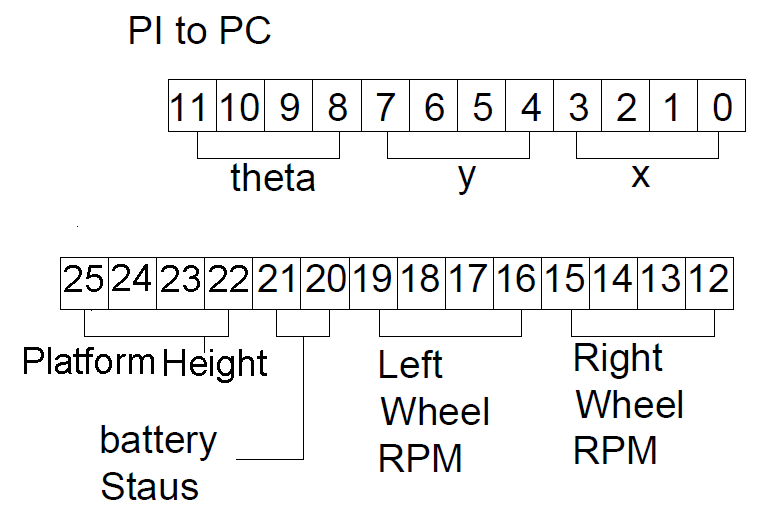
\includegraphics[width=\linewidth,keepaspectratio]{Chapter5/fig/bitconfig2}
   		\captionof{figure}{Data from the robot to PC}
   		\label{fig:recvBytes} 
   \end{minipage}
	
\end{figure}

\subsection{Local onboard controller}
The  onboard computer which is Raspberry Pi running raspian (linux) os receives  command from the remote station and controls the robot hardware through customized c++ application.
The Raspberry Pi  is daisy chained to the four Maxon make, EPOS2 motor controllers/drivers. The communication between the onboard computer and the first Maxon controller is over usb/RS232 interface using Maxon's proprietorial protocol~\cite{maxonrs232}. The first controller serves as CAN master for the rest of the controllers. The rear wheel motor drivers were configured in velocity servo loop. The drivers for steering and the z-axis motors were configured in position control loop.  The camera mounted on the mobile robot  and Raspberry Pi  were connected over Ethernet via a wireless hub. The wiring diagram of the robot is given in Figure \ref {fig:wiring}. Since the onboard camera is connected to the wireless network directly, it does not interfere with the command loop between the Raspberri Pi and the PC. 
\begin{figure}
	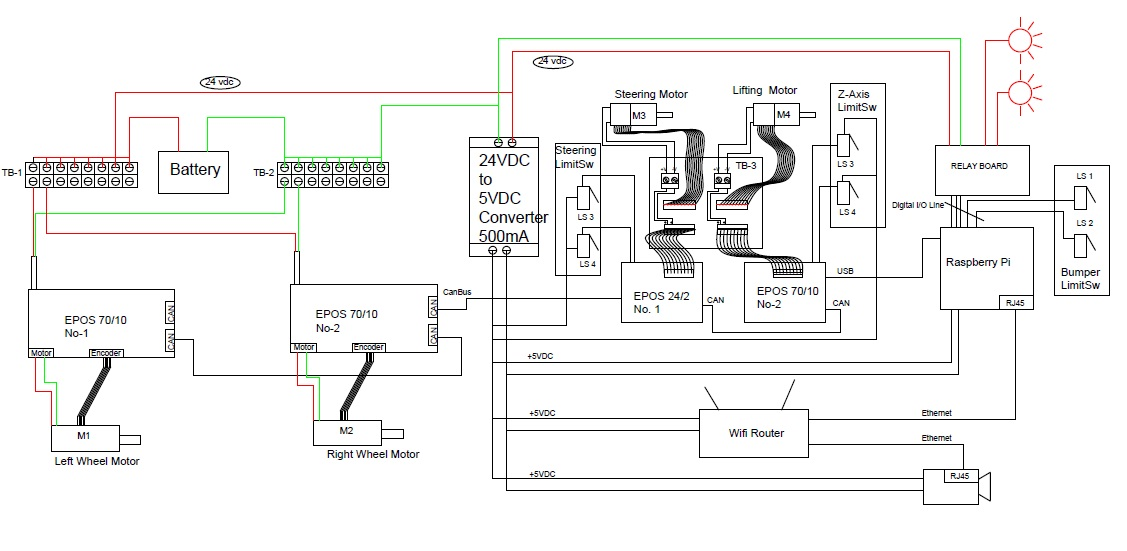
\includegraphics[width=\linewidth,keepaspectratio]{Chapter5/fig/RobotSideWiring}
	\captionof{figure}{Wiring  diagram of the WMR }
	\label{fig:wiring} 
\end{figure} 

The mobile robot is teleoperated using position-speed command as in \cite{farkhatdinov2007hybrid}.  The workspace for the mobile robot was assumed  infinite compared to the input device. In case of manipulators position-position, control approach is generally used with scaling. In this case,  the mixed approach was used. The steering angle was controlled in position-position mode whereas the mobile robot's speed was controlled by foot pedal's position, i.e. in  position-velocity mode. This can be given by the following equation: 
\begin{equation}
	\begin{pmatrix}
	V\\\theta_S
	\end{pmatrix}=
	\begin{pmatrix}
	K_v & 0\\0 & K_s
	\end{pmatrix}
	\begin{pmatrix}
	\tilde{X_p}\\
	\tilde{\Theta_s}
	\end{pmatrix}
\end{equation}
where $\tilde{X_p}$ is the displacement of pedal, $\tilde{\theta_s}$ is the twist of steering wheel, $K_v$ and $K_s$ are the proportionality constants, $V$ is the velocity of point $O_3$   and $\theta_s$ is the displacement of the steer motor. These proportionality constants are derived  based on extreme limits. They are  listed in Table \ref{tbl:propCnst}. 

\begin{table}[!htbp]
	\caption{Proportionality constant table} 
	\label{tbl:propCnst}
	\centering
	\begin{tabular}{l l l l l}
		\hline
		Robot  & range & Joy-Stick& range & parameter \\
		parameters& & Parameter & & Value\\
		\hline
		$\theta_s$ & -60 to +60 & $\tilde{\Theta_s}$ & $-90^o$ to $90^o$ & $K_s=2/3$\\
		$V$ & 0 to +60 mm/sec & $\tilde{X_p}$ & 0 to 30mm & $K_v=2$\\
		\hline
	\end{tabular}	
\end{table}


\subsection{Details of the motor controller}
Three EPOS2 controllers from Maxon Motors were used to control the mobile robot's rear wheel velocity and the steering gears position. Each controller can control one motor. The overall architecture of the controller  as given in \cite{maxonAutoTune}, \cite{maxonAppNotesPosition}  is shown  in  Figure \ref{fig:EPOS4}.
  \begin{figure}
	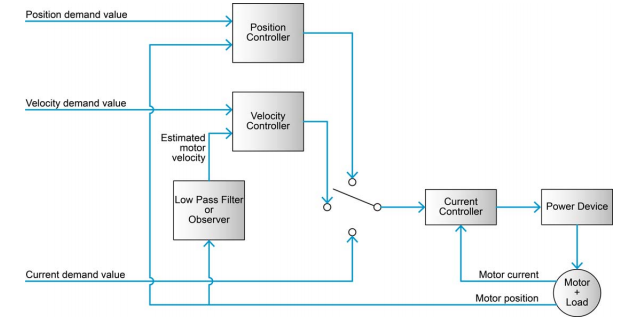
\includegraphics[width=\linewidth,keepaspectratio]{Chapter5/fig/overallcontorl}
	\captionof{figure}{Block digram of EPOS4 controller  }
	\label{fig:EPOS4} 
\end{figure}
 The controller can be configured in either current, position or velocity control mode. The inner most current loop controls the torque of the motor.
 The current feedback loop shown in Figure \ref{fig:curloop} is a Proportional Integrator (PI) controller, running at 25KHz and the transfer function of the PI block is given as \ref{eqn:curLoop}. 
 \begin{equation}
 	C(s)=K_p + \frac{K_I}{s}
 	\label{eqn:curLoop}
 \end{equation}
 where $K_p$ and $ K_I$ are the proportional and integral gains.
 
 
 \begin{figure}
 	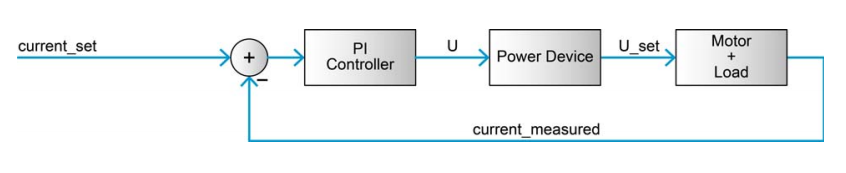
\includegraphics[width=\linewidth,keepaspectratio]{Chapter5/fig/currentLoop}
 	\captionof{figure}{Current control block }
 	\label{fig:curloop} 
 \end{figure}
 
 
  The rear motor controllers are configured in the velocity control mode.  The block digram  of the velocity loop is given in Figure \ref{fig:velloop}. The velocity controller is a PI controller with  velocity and acceleration feed-forward. 
  \begin{figure}
  	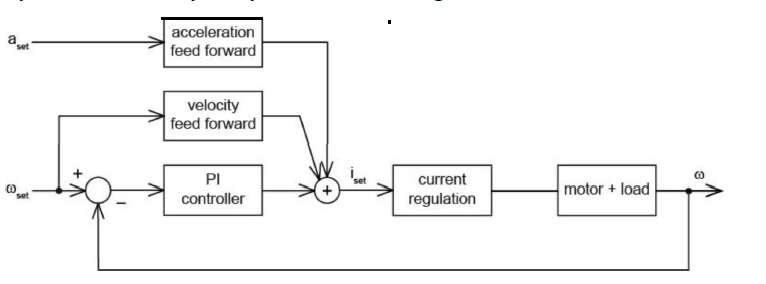
\includegraphics[width=\linewidth,keepaspectratio]{Chapter5/fig/velLoop}
  	\captionof{figure}{Velocity control bolck  }
  	\label{fig:velloop} 
  \end{figure}
  The transfer function $V(s)$ of the velocity loop PI block is given by
  \begin{eqnarray}
  V(s)=K_{p\omega}+\frac{K_{I\omega}}{s}
  \end{eqnarray}  where $K_{p\omega}$ and  $K_{I\omega}$ are  proportional and integral gains for velocity, respectively.   The sampling rate of the  velocity loop is 2.5 KHz. The feedforward acceleration and  velocity was used to compensate for the known inertial load and  viscous frictional load  \cite{maxonAppNotesPosition} respectively.   Velocity is estimated from differentiation of  the position data, the low-pass filter  in Figure \ref{fig:EPOS4}  eliminates noise due to differentiation. The transfer function $H(s)$ for the  low-pass filter is given by
  \begin{equation}
  H(s)=\frac{1}{1+\frac{K_{p\omega}}{48K_{I\omega}}}
  \end{equation} 
  
  The gain values used for each rear motor in  the velocity control mode is listed in Table \ref{tb:motorPara}. No acceleration or velocity feedforward  was used. These parameters were determined by auto tuning.  
  

  	  \begin{table}[!htbp]
  		\caption{Parameters for left and right rear wheel motor controllers  }
  		\label{tb:motorPara}
  		\centering
  		\begin{tabular}{c c c c}
  			\hline
  			\emph{Gain}  & \emph{ Right motor}  & \emph{ Left motor}& \emph{Unit} \\
  			\emph{ Parameter}  & \emph{ Value} & \emph{ Value} & \emph{\space} \\
  			\hline
  			$K_p$  & 300 & 230 &  $\frac{mV}{A}$ \\ 
  			$K_I $ & 100 & 53 & $\frac{mV}{A.mS}$ \\
  			$K_{P\omega}$& 1000 & 5182 & $ \frac{mA.sec}{rad}$\\
  			$K_{I\omega}$&100 & 425& $\frac{mA}{rad}$\\
  			\hline
  		\end{tabular}
  	\end{table}






The steering motor was in position control mode. The block digram is shown in Figure \ref{fig:posloop}. It is a PID controller with transfer function given as 
\begin{equation}
P(s)=K_{PP}+K_{IP}s+\frac{K_{DP}s}{1+\frac{K_{DP}}{10 K_{PP}}s}
\end{equation}
where $K_{PP}$, $K_{IP}$ and $K_{DP}$ are position proportional, integral and derivative gains respectively. The velocity feed-forward $F_{\omega P}$ and acceleration feed-forward $F_{\alpha P}$ were used in position control loop to take care of viscious friction and known inertial load. The gains for controller were decided using auto tuning software provided by Maxon Motors. The values are reported in Table \ref{tb:steer}.
\begin{figure}
	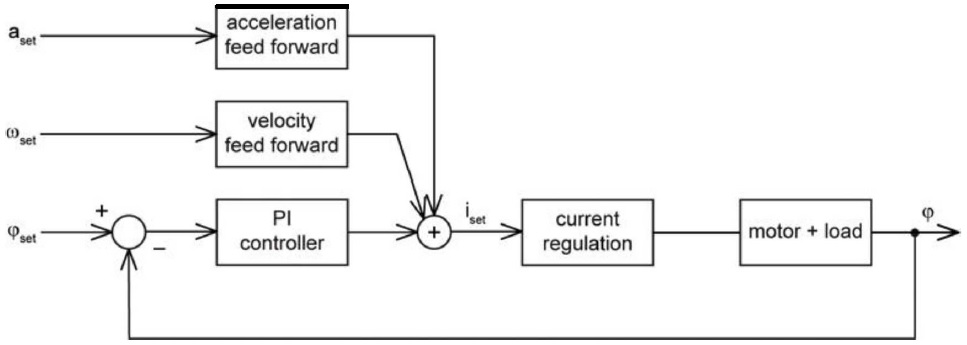
\includegraphics[width=\linewidth,keepaspectratio]{Chapter5/fig/posLoop}
	\captionof{figure}{Position control bolck  }
	\label{fig:posloop} 
\end{figure}
\begin{table}[!htbp]
	\caption{ Parameters of steering motor controller }
	\label{tb:steer}
	\centering
	\begin{tabular}{l l l}
		\hline
		\emph{Gain Parameter}  & \emph{ Value} & \emph{Unit} \\
		\hline
		$K_p$  & 537 &  $\frac{mV}{A}$ \\ 
		$K_I $ & 307 & $\frac{mV}{A.mS}$ \\
		$K_{PP}$& 128 & $ \frac{mA.sec}{rad}$\\
		$K_{IP}$&663&$\frac{mA}{rad}$\\
		$K_{ID}$&200&$\frac{mA}{rad}$\\
		$F_{\omega P}$& 0& $ \frac{mA.sec}{rad}$\\
		$F_{\alpha P}$& 54& $ \frac{mA.sec^2}{rad}$\\
		\hline
	\end{tabular}
\end{table}
\section{Control Algorithm }
This section discusses in detail the algorithm running on the onboard controller.  Command received by the controller was parsed to extract the velocity  and the steer angle  information. They were suitably scaled to get command velocity  $V$ in mm/sec, and steering  angle $\theta_s$ in radians.  It may be noted that the velocity $V$ corresponds to the velocity of point $O_r$ the reference point of the mobile robot.  Next the set point for each motor was calculated  and sent to individual drive. The algorithm is listed below and the block digram for the same in Figure \ref{fig:ControlBlock}
\begin{figure}[h]
	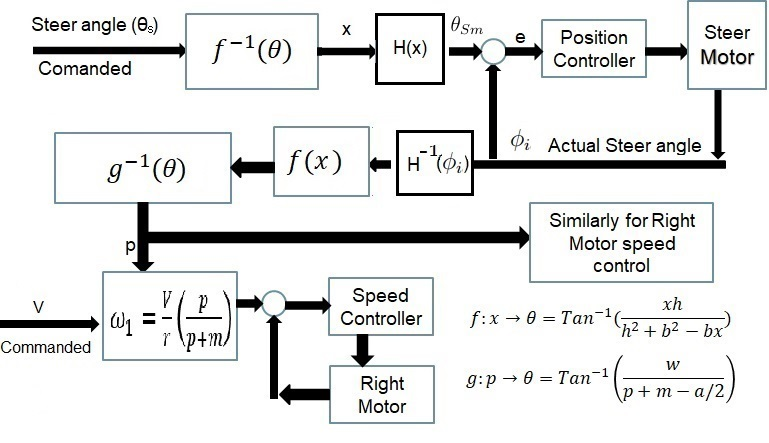
\includegraphics[width=\linewidth,keepaspectratio]{Chapter5/fig/BlkDigLocal2}
	\captionof{figure}{Block digram of WMR controler}
	\label{fig:ControlBlock} 
\end{figure}

\begin{enumerate}
	\item Calculate the setpoint for steering motor $\theta_{SM} $ based on $\theta_s$.
	\item Read the current steering  angle $\phi_{ic}$.
	\item Calculate the velocity setpoints $\omega_{i}$ and $\omega_{o}$ of  rear wheels based on the $V$ and $\phi_{ic}$.

	
	\item Command  setpoints $\omega_{i}$, $\omega_{o}$ and $\theta_{SM} $ to each motor. 
\end{enumerate}
The above loop is repeated every 50 mSec.

It may be noted that the steer angle command received from the control station is not directly sent to the steer motor as set point after suitable scaling. The steer set point is based on the current rear wheel velocities. This is important as the response time of the  motors are different. The above methodology helps  minimize the deviation  from the Ackerman  steering condition even during transit condition, particularly, in case of large change in commanded $v$ and $\theta_s$. 
Each block in Figure \ref{fig:ControlBlock} is discussed next. 

 It may be noted that the $\theta_s$ always refers to the steer angle of the inner front wheel $\phi_i$  and $V$ refers to $O_r$ as shown in Figure \ref{fig:KenVec}, i.e.
 \begin{equation}
	 \theta_s =\phi_i
 \end{equation}
 The set point of the steering motor at the output of  gear box $\theta_{SM}$ is given by equations \ref{eqn:sterineq1} and \ref{eqn:sterineq2}  based on the geometry of Davis steering gear \cite{TOMBook}.
\begin{equation*}
 \tan\phi_i=\frac{xh}{h^2+b^2-bx}
\end{equation*}
or
\begin{eqnarray}
f(\phi_i): x=\frac{\tan\phi_i (h^2+b^2)}{h+b \tan\phi_i }
\label{eqn:sterineq1}
\end{eqnarray}
\begin{figure}
	\begin{minipage}[t]{0.6\textwidth}
		\centering
		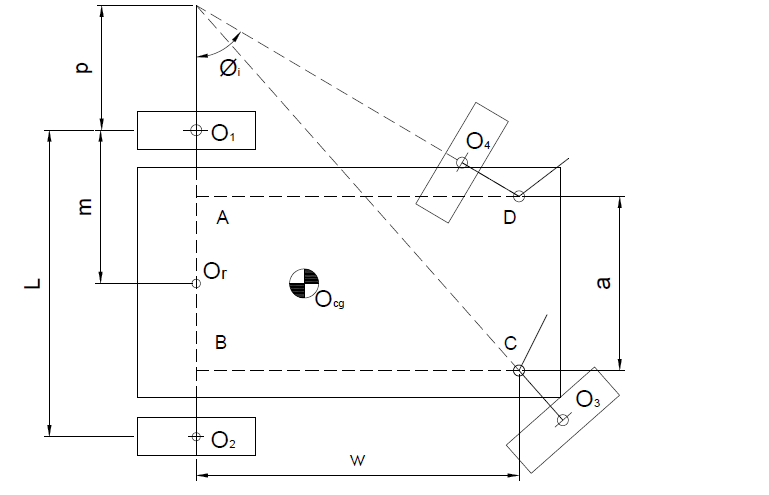
\includegraphics[width=5in]{Chapter5/fig/kinvec} 
		\caption{Ackerman Steering Condition}\label{fig:KenVec}
	\end{minipage}
	%\hfill
	\begin{minipage}[t]{0.7\textwidth}
		\centering
		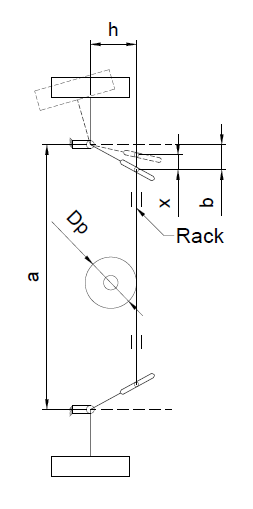
\includegraphics[height=3.5in]{Chapter5/fig/davisgear} 
		\caption{Davis Steering Gear}\label{fig:steering_gear_train}
	\end{minipage}
\end{figure}
where $x$ is the displacement of the rack and $h$ and $b$ are link lengths. The rack is connected to the steering motor by pinion of pcd $D_p$ (30mm) as shown in  Figure \ref{fig:steering_gear_train}. Therefore, the steering motor angle,  $ \theta_{Sm}$, is given below as
\begin{eqnarray}
H(x): \theta_{Sm}= x \frac{360}{\pi D_p}
\label{eqn:sterineq2}
\end{eqnarray}
 
Next,  the equation relating current steer angle $\phi_{i}$   and rear wheel  set point velocities $\omega_{RS}$ and $\omega_{LS}$ is presented. From the geometry of Figure \ref{fig:KenVec}, one gets
\begin{align}
\nonumber \tan\phi_{i} &=\frac{\bar{BD}}{\bar{OB}}=\frac{w}{p+m-a/2}\\ 
g:\phi_{i} \rightarrow p,\quad \quad p &= \frac{w}{\tan\phi_{c}}-m + \frac{a}{2}
\label{eqn:pFromTheta}
\end{align}
%similarly for the inner wheel we get  
%\begin{equation}
%p = \frac{w}{\tan\theta_i}-m - \frac{a}{2}
%\end{equation}
Now using Equations \ref{velO1} and \ref{omegaPlat}  in equations relating the right and left wheel velocities to the WMR platform angular velocity $\omega_3$ and velocity, $V$, of the reference point $O_r$, presented below
\begin{align*}
\dot{O_r}&=\dot{O_i}+\omega_3 \times (O_r-O_i)\\
\dot{O_r}&=\dot{O_o}+\omega_3 \times (O_r-O_o)
\end{align*}
 We get the  velocity of each rear wheel as  
\begin{align}
\nonumber \omega_i&=\frac{Vp}{r(p+m)}\\
\nonumber \omega_o &=\frac{V(p+2m)}{r(p+m)}
\end{align}
Using the above equations and Equation \ref{eqn:pFromTheta},  the setpoints for the rear wheels are as follows 
\begin{equation}
\omega_i =\frac{V}{r}\frac{( \frac{w}{\tan\theta_o}-m + \frac{a}{2})}{ \frac{w}{\tan\theta_o}-m + \frac{a}{2}+m}
\end{equation}
\begin{equation}
\omega_o =\frac{V}{r}\frac{( \frac{w}{\tan\theta_o}-m + \frac{a}{2})+2m}{ \frac{w}{\tan\theta_o}-m + \frac{a}{2}+m}
\end{equation}
 

 
%\begin{itemize}
%\item calibration of steer data and wheel velocity
%\end{itemize}

\subsection{Wheel odometery }
The dead reckoning odometery can be performed based on either the differential drive or Bicycle model. In the present case, we use the differential drive model was used/ Where the rear wheel velocities were used to determine the position and orientation of the mobile robot. The position here means the position of the reference point $O_r$. The steps are followes.
\begin{enumerate}
	\item calculate $V$ and $\omega_3$ from current wheel velocities $\omega_1$  and  $\omega_2$  using equations \ref{omegaPlat} and \ref{velPlat} with $a=0$.
	\item integrate $V$ and $\omega_3$ over time step.
\end{enumerate}
If $x(t)$, $y(t)$ are the coordinate of $O_r$  and  $\beta(t)$ be the orientation of the robot with some global coordinate system, the kinematic model of the differential wheel robots is given by \cite{campion1996structural}  
\begin{equation}
\label{eqn:DiffKinModel}
\begin{pmatrix}
\dot{x}\\\dot{y}\\\dot{\beta}
\end{pmatrix}=
\begin{pmatrix}
\cos\beta & 0\\
\sin\beta & 0\\
0&1
\end{pmatrix}
\begin{pmatrix}
V\\\omega_3
\end{pmatrix}
\end{equation}
Equation \ref{eqn:DiffKinModel} is numerically integrated for time $\delta t$ using the following expressions:
\begin{align}
\label{eqn:odo1}
 x(i+1)&=x(i)+\delta t~ V(i)\cos\beta(i);\\
 \label{eqn:odo2}
y(i+1)&=y(i)+\delta t~V(i)\sin\beta(i);\\
\label{eqn:odo3}
\beta(i+1)&=\beta(i)+\delta t~\omega_3(i);
\end{align}
where $i$ is at time step $t_i$. Next,  the actual odometric results for the vehicle moving in a circle and a straight line are presented.
\begin{figure*}
	\begin{minipage}[t]{0.5\textwidth}
		\centering
		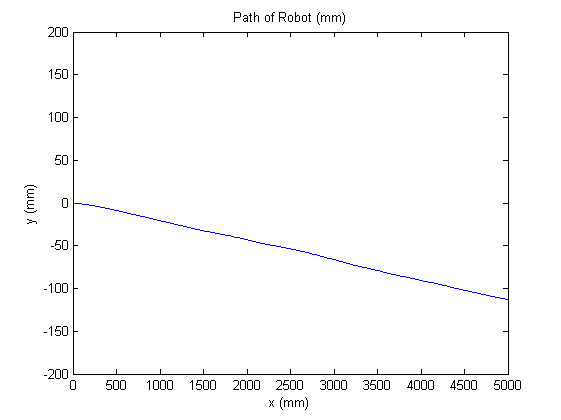
\includegraphics[width=3.0in]{Chapter5/fig/Line} 
		\caption{Tracing a line}\label{fig:line}
	\end{minipage}
	\hfill
	\begin{minipage}[t]{0.5\textwidth}
		\centering
		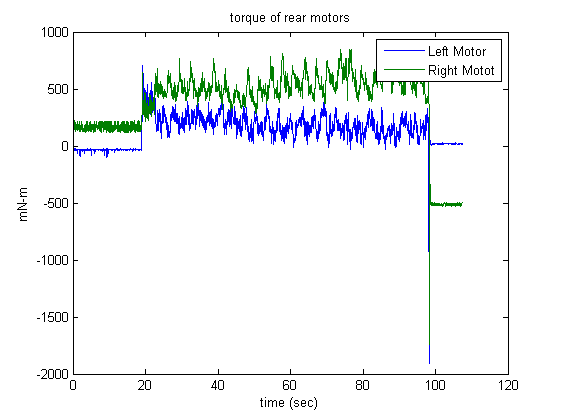
\includegraphics[width=3.2in]{Chapter5/fig/linTorq} 
		\caption{Motor torque}\label{fig:linTorq}
	\end{minipage}
	\begin{minipage}[t]{0.5\textwidth}
		\centering
		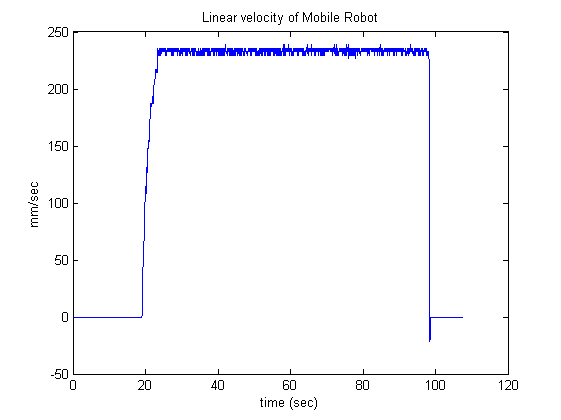
\includegraphics[width=3.1in]{Chapter5/fig/linVel} 
		\caption{Linear velocity}\label{fig:linVel}
	\end{minipage}
	\hfill
	\begin{minipage}[t]{0.5\textwidth}
		\centering
		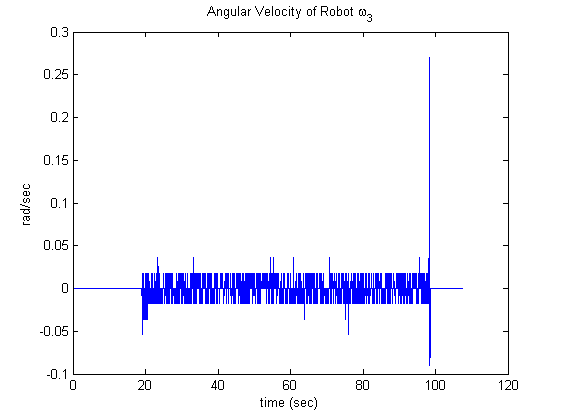
\includegraphics[width=3.1in]{Chapter5/fig/linOmega} 
		\caption{Angular velocity}\label{fig:linOmega}
	\end{minipage}
	%\caption{Linear motion of  WMR}
\end{figure*}

As seen in the graph of Figure \ref{fig:line} there is a lateral shift in the robots path calculated using odometry.  There is a linear shift too, which can observed due to longer path calculated by odometry. The lateral shift of 200 mm and a linear shift of 300 mm for 15000 mm long path was calculated. This clearly indicates slip in the wheels. The torque curves also shows that one wheel is more loaded that the other this is expected as the battery weight was on one side of the robot.
\begin{figure}
	\begin{minipage}[t]{0.5\textwidth}
		\centering
		\includegraphics[width=3.5in]{Chapter5/fig/circleOdo} 
		\caption{Tracing a circle}\label{fig:circle}
	\end{minipage}
	\hfill
	\begin{minipage}[t]{0.5\textwidth}
		\centering
		\includegraphics[width=3.2in]{Chapter5/fig/cirTorq} 
		\caption{Motor torque}\label{fig:cirTorq}
	\end{minipage}
\vfill 
\begin{minipage}[t]{0.5\textwidth}
	\centering
	\includegraphics[width=3.1in]{Chapter5/fig/cirVel} 
	\caption{Linear velocity}\label{fig:cirVel}
\end{minipage}
\hfill
\begin{minipage}[t]{0.5\textwidth}
	\centering
	\includegraphics[width=3.1in]{Chapter5/fig/cirOmega} 
	\caption{Angular velocity}\label{fig:cirOmega}
\end{minipage}
	%\caption{Circular motion of  WMR}
\end{figure}

\subsection{ Remote control station}   
The operator controls the vehicle from a local station away from the robot over a wireless network. The control station consists of a desktop computer running Windows XP. A steering wheel and two foot switches are connected to the desktop. The steering wheel sets the steering of the remote mobile robot and the footpadel is used to set the velocity $V$ of the robot. A push button in the steering wheel is used to reverse the direction of motion of the robot.

The screen of the desktop displays  video streaming  from the mobile robot's on board camera. A graphical user  interface (GUI) shown in Figure \ref{fig:Gui} displays the robot's parameters such as current steer angle, velocity of each rear wheels and the position of the z-axis. Buttons on the GUI operates the z-axis, head lamps, etc.

\begin{figure}
	\includegraphics[width=\linewidth,keepaspectratio]{Chapter5/fig/gui}
	\captionof{figure}{User interface for teleoperation }
	\label{fig:Gui} 
\end{figure}


%\subsubsection{Control of Z platform}
%Decentralized control technique treats the manipulator and the platform as two different system. The inter-coupling forces are treated as external forces on the system. The dynamics equation of the mobile manipulator can thus be split as follows [3].
%\section{Admissible path}
%\section{Trajectory Tacking}


\section{Summary}
In this chapter, the control architecture of the mobile manipulator has been presented. The  algorithm used  to move the robot was discussed in detail. The odometry used for pose estimation of the robot was also presented with the experimental results. 



\cleardoublepage

\chapter{Simulation Time Delay Tele-operation}
\label{c7_DI_equimomental}
In this chapter simulation of a teleoperated mobile platform is presented. In tele-operation the human operators observe a remote scene through camera/s, and manipulating the local steering wheel and accelerator paddle as shown in figure \ref{fig:teleoperation} . The command is transmitted to the mobile robot over wireless network. The operator response is based on the latest feedback images from the cameras. The simulation results are presented of robots behaviour for the delayless and delay transmission network.
\begin{figure}
	\includegraphics[width=\linewidth,keepaspectratio]{Chapter6/fig/teleoperation}
	\captionof{figure}{Teleoperation  Architecture }
	\label{fig:teleoperation} 
\end{figure}

\section{Tele operation simulation architecture}
The standard kinematic model as described in \cite{campion1996structural} of the mobile platform is used for the simulation. This is justified as  the vehicle is expected to move at relatively slow speed. The inputs to the model are the left and right rear wheel velocities. The front wheels are steered to satisfy the Ackerman condition as presented in **** and are assumed to attain the desired angle instantaneously. Therefore the robot can be treated as differential drive robot.  The kinematic model of the platform is presented below
\begin{equation}
\begin{pmatrix}
\dot{x}\\ 
\dot{y}\\ 
\dot{\theta}
\end{pmatrix}
=
\begin{pmatrix}
\sin \theta & 0 \\
-\cos \theta & 0 \\
0& 1
\end{pmatrix}
\begin{pmatrix}
r/2 & r/2\\
1/b & -1/b
\end{pmatrix}
\begin{pmatrix}
\dot{\phi_L}\\
\dot{\phi_R}
\end{pmatrix}
\end{equation}


Where ,  $b$is the distance between the rear wheels,$r$ wheel radius. $\dot{\phi_R}$ and $\dot{\phi_L} $ are the left and right wheel rotational velocity. 

The operator station sends the command $u_1$ and $u_2$ over the wireless network, in general it will be delayed by $\delta$ time. These commands are interpreted by the robot controller as the left and right wheel velocities.  Therefore by taking the time delay into consideration we can write
\begin{equation}
\begin{pmatrix}
\dot{\phi_R}(t) \\
 \dot{\phi_L}(t)
\end{pmatrix}
=
\begin{pmatrix}
u_1(t-\delta)\\
u_1(t-\delta)
\end{pmatrix}
\end{equation}

The control inputs to the mobile robot  $u_1$ and $u_2$ are generate by the operator based on the visual data available to him. We next present the model of the human operator to be used for simulation the complete loop.


\section{Modeling the human operator}
In order to simulate the teleoperation loop we need a mathematical model of human operator. The mathematical  modelling of the operator`s action is modelled assuming a car driving metaphor. The video feedback, which the he receives of the remote environment, give him the idea of the vehicles  position and the tentative next goal point (p) based on a lookahead distance (l). He then constructs a  virtual path mentally and tries to manoeuvre or steers the robot to follow that path as shown in figure \ref{fig:drivingStratagy}. As he moves forward the goal point keeps changing until he reaches the desired location. This methodology of path tracing is known as pure pursuit \cite{coulter1992implementation} or following the carrot strategy. 
\begin{figure}
	\includegraphics[width=\linewidth,keepaspectratio]{Chapter6/fig/mentalMap}
	\captionof{figure}{Assumed driving strategy  }
	\label{fig:drivingStratagy} 
\end{figure}

The mathematical model is derived next.

\section{Simulation Results }
\section{Predictive Model based Feedback}
\subsection{Using Dynamic model of vehicle}
\subsection{Kalman Filter with odometer data and Accelorometer?}


\section{Summary}
In this chapter, 

\cleardoublepage
\chapter{Time Delay Compensation and Predictive Display}
\label{ch_7:PDsply}
In the last chapter, it is shown using simulation that time delay between the remote and local stations leads the system towards instability. In this chapter, first  predictive model controller for time delayed teleoperation is presented. Associated issues of time delay on human performance are then highlighted. To alleviate the problem of time delay in visual feedback, predictive display using a RGB-Depth sensor is  implemented.

\section {Time Delay Compensation}
Simulation of time delayed system with pure pursuit model for human controller was presented in Chapter \ref{c6_simulation}.  Stability aspects with input delay to the human model was pointed out. In paper by Ollero \cite{ollero1995stability}, stability of pure pursuit with input delay is presented and for completeness briefly discussed in Appendix \ref{appendix_b}.   In view of the above theoretical analysis and the simulation results presented in chapter \ref{c6_simulation}, it is required to design  a stabilizing controller to take care of large delays, e.g.,  0.8 sec. One such design based on model  predictive control is presented next.

 \begin{figure}
 	\includegraphics[width=\linewidth]{Chapter7/fig/Smith_predictor}
 	\caption{Smith Predictor \cite{smith1959controller}}
 	\label{fig:Smith}
 \end{figure}
 
 One of the earliest predictor based controller for Linear system with time delay  was proposed by Smith \cite{smith1959controller} called the Smith Predictor or Smith Controller. The schematic of the smith controller is shown in Figure \ref{fig:Smith}. There are two loops, the inner and the outer loop, where $G(z)$ is the plant, $C(z)$ is the stabilizing controller  for the plant without delay, $\hat{G}(z)$ is the model of the plant.  As can be seen from the Figure \ref{fig:Smith} that during the period (k time unit ) when the feedback (output) is not available the model of the plant is used to predict the actual plant behaviour and generate the control signal accordingly. 
 
 In the presented case, the plant is the mobile robot developed in this PhD research. The block digram shown in Figure \ref{fig:blockdigTimeDelay} depicts the architecture of time delayed system which is applicable to the current mobile robot and the local station. The teleoperation  over wireless network for our system   resulted in a delay of $T_1= 500~ms$ with update frequency of 2Hz.  The delay was caused due to large amount of data being transmitted as  video feedback from the robot's onboard camera. Figure \ref{fig:delayphoto} shows the measured delay in the video link. The frequency of odometric and control  data exchange between the two stations was at the rate of 20Hz, i.e., a delay $T_2=50~ms$ only. This  loop runs  independent of the video feedback link.  It may be noted that $T_2<<T_1$.
 \begin{figure}[ht]
 	\centering
 	\begin{minipage}{0.55\textwidth}
 		\centering
 		\includegraphics[width=.9\linewidth,keepaspectratio]{Chapter7/fig/BlockTimeDelay}
 		\captionof{figure}{Block digram of time \\delayed system}
 		\label{fig:blockdigTimeDelay}
 	\end{minipage}
  	\begin{minipage}{0.40\textwidth}
 	\centering
 	\includegraphics[width=\linewidth,keepaspectratio]{Chapter7/fig/delayMeasureNew}
 	\captionof{figure}{Delay measurment}
 	\label{fig:delayphoto}
 \end{minipage}%
 \end{figure} 


\subsection{Proposed Controller}
The proposed control strategy to mitigate the effect of time delay is to predict the current position from the last known position, based on the delayed video image; using  the dynamic model of the mobile robot.  As shown in Figure \ref{fig:SmithRobot}, let us assume that we are at time $t+\delta$, but the latest pose  data of the robot available is that of at time $t$. The present pose at time $t+\delta$ was predicted  using  the dynamic model  of the robot derived in Chapter \ref{c4_Dynamics}, Equation \ref{CE}, and presented here again for convenience. 
\begin{equation}
\label{CE2}
\quad I(\theta)\ddot{\theta}=C(\theta,\dot{\theta})\dot{\theta}+\tau
\end{equation}
It may be noted that the dynamic model uses torque $\tau$ as its input, whereas the local station which uses pure pursuit for simulation of  human action   generates linear and angular velocities of the robot,  $v$ and $\omega$ as shown in Figure \ref{fig:SimBlock}. This is taken care by first converting $v \equiv\dot o_3$ and $\omega\equiv\omega_3$ to rear wheel velocities using Equations \ref{omegaPlat} and \ref{velPlat}. The rear wheel velocities  are then used in PI controller of the rear wheel motors to generate the $\tau$ for Equation \ref{CE2}.

This predicted position is given to the pure pursuit algorithm to generate required control outputs for the remote robot. In the simulation, it was assumed that this control inputs reaches the remote robot instantaneously, as $T_1>> T_2$. As discussed in the   Kinematic model of Chapter \ref{c6_simulation}. Equation \ref{eqn:KinematicModelOfRobot} was used to simulate the remote robot.
 \begin{figure}
	\includegraphics[width=1.2\linewidth]{Chapter7/fig/robotPredictPos}
	\caption{Smith predictor applied to the developed mobile robot}
	\label{fig:SmithRobot}
\end{figure}
 \begin{figure}
	\includegraphics[width=\linewidth]{Chapter7/fig/Sumilation_BlkDgm}
	\caption{Simulation block Digram}
	\label{fig:SimBlock}
\end{figure}
\subsection{Simulation algorithm and  results} 
The simulation scheme is  shown in block digram of Figure \ref{fig:SimBlock}. The algorithm  is explained  below.

\begin{algorithmic}[1]
	\State Convert the path from global coordinate system (CS) to Robot's Local Coordinate System based on the  current pose  $(x,y,\theta)$ of the robot.
	\State With a given look ahead distance ($l$) search for a goal point on the path.
	\State Determine the turning radius ($r$) using Equation 6.5 
	\State Calculate $\omega$ using turning radius ($r$) and given Linear Velocity $v$
	\State Command Robot $\omega$ and  $v$
	\If  {new pose of the robot is available from remote station}
		\State Update robot pose $(x,y,\theta)$
	\Else
		\State Calculate the predicted pose of the robot  based on command given in Step 4, and using dynamic model of therobot given by Equation \ref{CE2}.
		\State Update robot's pose $(x,y,\theta)$ 
	\EndIf
	\State\textbf{ Goto} Step 1
\end{algorithmic}	
 Simulation was carried using Matlab. Differential equation solver \textit{"Ode24"} was used to solve Equations \ref{eqn:KinematicModelOfRobot} and \ref{CE2}.  The desired path  was a circle of radius 5m centred at origin of the global coordinate system. The human action was modelled with look ahead distance $l$ of 0.5m and linear velocity $v$ of $0.5~m/s$. The initial position of the robot was (4.5,0.0). 
 The  robot's motion  under feedback delay of 0.5 sec and 0.8 sec, i.e.,  $T_1=0.5~sec$ and $T_1=0.8~sec$,  are shown in  Figures \ref{fig:PreDelay500plot} and \ref{fig:PreDelay800plot} respectively.   It is seen that oscillation are no more visible at delay of 0.5 sec  and   0.8 sec. The system shows no instability. 

 \begin{figure}[h]
 	 \begin{minipage}[T]{0.5\linewidth}
 	 	\centering
 	 	\captionsetup{justification=centering}
 		\includegraphics[width=\linewidth,keepaspectratio]{Chapter7/fig/withPrediction05dely}
 		\captionof{figure}{Time delay $T_1=.5~sec$\\ and $T_2=0$ }
 		\label{fig:PreDelay500plot}
 	\end{minipage}
 \hfill
 	\begin{minipage}[T]{0.5\linewidth}
 		\centering
 		\captionsetup{justification=centering}
		\includegraphics[width=\linewidth,keepaspectratio]{Chapter7/fig/withPrediction08delay}
		\captionof{figure}{Time delay  $T_1=.8~sec$ \\ and $T_2=0$ }
		\label{fig:PreDelay800plot} 
 	\end{minipage}
 \end{figure} 


The above results show that model-based prediction of the robot's pose helps in removing the instability of the system. In  actual teleoperation, the operator's control actions are based on the visual display available to him.  The delay in visual feedback results in inefficient operator's performance as the person tends to adopt a wait and watch policy to see the effect of his control action. In the next section,  an implementation and adaptation  of above discussed \textit{model based prediction }  for  visual display feedback is presented.   
  
\section{Predictive Display}
As indicated in Chapter \ref{c2_LitRev} on Literature survey,  the delay of visual feedback leads to inefficient and unstable performance of a teleoperated system. There are two major methods to overcome time delay induced problems in teleoperation. One is to use \textit{supervisory control} and the other is \textit{predictive display}. The second methodology, i.e., the Predictive Display, was adapted here. This is because it is more intuitive to human operators, and the onboard controller  required on the mobile robot is very much simplified.  

  
Predictive display has been defined as using the computer for extrapolating the display forward in time \cite{sheridan}. In this, a local model of the remote scene is used to predict and render the remote scene in response to operator's command. It replaces the delayed video feedback with extrapolated synthesised  image of the remote environment. This enables the operator to perform the task normally. Predictive display has been implemented in the past using different sensors such as monocular camera fixed on the wall, camera mounted on the robot arm, fusion of Lidar scanner and RGB camera, etc. 
The proposed approach here is to use a low-cost  Kinect Sensor from Microsoft Inc. to generate the 3-D model of the remote environment and use kinematic model of the mobile robot to predict the motion of the actual robot on the 3-D model of the environment  to generate a delay-free estimated image of the remote scene operator.

\subsection{Kinect Sensor }
\begin{figure}
	\includegraphics[width=\linewidth,keepaspectratio]{Chapter7/fig/kinect}
	\caption{Kinect Sensor from Microsoft}	\label{fig:Kinect}
\end{figure}
Kinect sensor from microsoft is shown in Figure \ref{fig:Kinect}. The hardware contains a normal RGB camera, a depth sensor and a four-microphone array, which are able to provide  RGB images,  depth signals, and audio signals simultaneously. The depth sensor comprises of an Infra Red (IR) projector and the IR camera. The IR projector casts an IR speckle dot of known  pattern into the 3-D scene while the IR camera captures the reflected IR speckles. To determine the depth, triangulation method is used.  Kinect is therefore an instance of a structured light depth sensor. More details concerning the structured light 3-D imaging technology can be found in \cite{geng2011structured}. 

The \textit{RGB camera}  delivers three basic colour components of the video. The camera operates at 30 Hz, and can offer images at $640\times480$ pixels with 8 bits per channel. The  \textit{3-D Depth Sensor} creates a depth map, which provides the distance information between the camera and an object. The sensor has a practical rang limit of 0.8m-3.5m distance, and outputs video at a frame rate of 30 frames/sec with the resolution of 640 x 480 pixels. The angular field of view is $57^o$ horizontally and $43^o$ vertically.
Number of different open source software libraries are available  which includes OpenNI \cite{openni}, Microsoft Kinect SDK  \cite{mssdk} and OpenKinect \cite{freenect} to access data from the Kinect sensor. OpenNi was used inn this research, as it is compatible with RTabMap, an Open Source Software used for reconstruction of the 3-D point cloud model of the  remote scene. 

\subsection{Onboard Data processing and transmission}
In teleoperation. the Kinect sensor mounted on the mobile robot was connected with the onboard Raspberry Pi single board computer with limited processing power. The onboard controller uses OpenNi library to interface with the kinect hardware.  The Kinect sensor has two separate cameras. The transformation between the camera centres are known and provided by the manufacturer. It therefore generates two streams, the colour and depth data. It is possible to send the two raw data streams over the network  without any processing at the robot's side. This  puts less stress on the onboard computer but requires high communication bandwidth. The other option is to stream \textit{ registered depth} data over the network. This requires less bandwidth as each pixel has both the colour and depth value associated with it when it is transmitted. Depth Registration requires minimal computing power. Known transformation between the two cameras was used to align the depth pixel and the colour pixel so that they correspond to the same point of the 3-D scene. This is referred to as \textit{depth registration} or \textit{image registration} in the literature. The word "depth" in the   \textit{depth registration} indicates  that the final image data is with respect to  the depth camera's frame. The second method was adapted here. The robot transmits registered depth data, i.e., the RGB and the Depth (RGB-D) values associated with each pixel to the control station over network. 


\begin{figure}
	\includegraphics[width=\linewidth,keepaspectratio]{Chapter7/fig/PredictorBlockDig}
	\caption{Predictive display architecture}	\label{fig:PDBLock}
\end{figure}

\subsection{3-D Reconstruction }
The registered depth data received at the operator-station was processed using the RTabMap library \cite{rtabmap} and 3-D Point Cloud data was generated. The details of the working of RTabMap can be found in \cite{labbertab} and \cite{labbe2013appearance}.  Point cloud map is a set of points in 3-D space derived using the camera model and the depth data associated with each pixel of the depth registered data sent from the mobile robot. Each new frame that arrives is added to the current data set after proper transformation. The transformation between the two frames of data was created by matching the common feature in the two frames. The RTabMap library thus outputs a set of 3-D point alongwith their RGB color. The coordinates of the points are always  with respect to camera coordinate frame. It may be noted that the registered depth image that has arrived was delayed by $T_1$ unit of time. So the local station always has a 3-D map w.r.t  the robot at $(t-T_1)$ sec.
 

\subsection{Extrapolation remote scene } 
The visual data present in the current frame is the view that the robot has seen $T_1$ seconds earlier. Let this data be denoted as $P(t-T_1)=Set\{P_k\}$. The point $P_i$ is associated with the coordinates ${Px_k,Py_k,Pz_k}$ and color data $c_k$. In order to predict the current scene that the robot might be seeing one needs to estimate the current position of the robot. The  architecture of the teleoperation shown in Figure \ref{fig:PDBLock} was used inthe developed mobile robot to accomplish the task.
 It has been stated earlier that the delay $T_2$ in exchange of command data and the wheel velocity data from the robot to the operator station was 20ms. It may thus be assumed that  using the odometric data in Equation \ref{eqn:odo1},~\ref{eqn:odo2} and \ref{eqn:odo3}, the current position of the robot was always known to the operator-station. This was performed by Odometric Block of Figure \ref{fig:PDBLock} by using Equations \ref{eqn:odo1},~\ref{eqn:odo2} and \ref{eqn:odo3} from time $t-T_2$ to $t$. Where $t$ denotes the current time and  with initial condition \[x(i=0)=0,~y(i=0)=0 ,~ \beta(i=0)=0\] and  \[ i=0 \text{ to } n;  \quad n=T_1/T_2\] 
 Let the predicted position of the robot at time $t$ be given by 
\[[x(i),~y(i) ,~ \beta(i)]\rightarrow [_v(t),y_v(t),\beta_v(t)]^T\]
This was basically the amount by which the robot has moved after the last video frame had arrived. Next, the transformation matrix, $T^c_r$ between the mobile robot's coordinate frame at point $O_r$ in Figure \ref{fig:KenVec} and the camera frame was used to calculate the change in pose of the camera. Since the points $P_i$ are in the camera frame their current coordinates ${P'x_i,P'y_i,P'z_i}$ was arrived at by using 
\begin{eqnarray}
\begin{pmatrix}
P'x_i \\ P'y_i \\P'z_i
\end{pmatrix}=T^c_r
\begin{pmatrix}
Px_i\\Py_i\\Pz_i
\end{pmatrix}
\end{eqnarray}
This new location of the points were then  projected onto the screen of the local operator, thus, giving him the estimated current view of the remote scene. 
 \begin{figure}[ht]
	\begin{minipage}{.5\textwidth}
		\includegraphics[height=4cm,keepaspectratio]{Chapter7/fig/pcdT}
		\captionof{figure}{PCD at time T }
		\label{fig:pcdt} 
	\end{minipage} 
	\begin{minipage}{.5\textwidth}
		\includegraphics[height=4cm,,keepaspectratio]{Chapter7/fig/pcdT_p}
		\captionof{figure}{Predicted Scene}
		\label{fig:pcdP} 
	\end{minipage}
\end{figure}
The view available at the operator station at time $t$ is shown in Figure \ref{fig:pcdt} which is $T_1$ sec old. Based on this old data, the predicted scene is shown in Figure \ref{fig:pcdP}.  The operator  sees  Figure \ref{fig:pcdP} instead of Figure \ref{fig:pcdt}.

With the predictive display model the operator was able to move the robot without\textit{ "wait and see"} stratagey adopted earlier. The motions were smooth and speed of operation improved.

\section{Summary}
In this chapter,  the model-based predictive control for control of mobile robot over time delayed network is presented. The stability of the control was verified using simulation. This model was then adopted for  teleoperation using visual feedback. Kinect sensor was used to generate the 3-D model of the remote environment in real time. The estimated position of the mobile robot using the odometry was used to project a synthesised image of the 3-D model of the remote environment.  


\cleardoublepage
\chapter{Conclusions}
\label{ch_8:Con}
%This chapter includes the thesis summary, major contributions and future scope of the work.
\section{Thesis Summary}
This thesis describes the design and development of a customized mobile manipulator developed at Bhabha Atomic Research Centre, Mumbai, India  for mapping radiation in different areas of Cyclotron building where human access is restricted during Cyclotron operation. The custom mobile manipulator is a four wheeled mobile robot with a vertical lifting platform on which the radiation detector is mounted. The mobile platform has two rear wheels individual coupled to   two motors and the front two wheels are mutually connected using motorized Davis steering mechanism.

   The first chapter describes the various types of mobile manipulator reported in literature and different areas in which mobile manipulators have been successfully used. The chapter also describes the motivation and requirement of a customized mobile manipulator.  Second chapter gives the literature review related to design, mathematical modeling and teleoperation setup of mobile robot which forms the complete system and is  the scope of this thesis. 

In chapter 3 the mechanical design, selection of motors and optimization  of steering mechanism to achieve minimum turning radius within the required space is discussed. The optimal location of CG for  the mobile manipulators so as to provide maximum traction as well as  stability over $30^o$ ramp is described.   It also discusses different lifting platform for vertical motion required by the sensor for scanning. Detail design  of scissor based lifting platform and its advantage with respect to the system requirements are discussed. 

The kinematic and dynamic modeling of the customized mobile manipulator is presented in chapter 4.  Natural orthogonal compliment method is used to derive the dynamic model of the wheeled platform. This analysis highlights the  effect of caster  offsets on the manuverability of a mobile platform. The need of having a positive drive for certain castor offsets are also brought in the analysis. This chapter also include the dynamic modeling and simulation of steering mechanism  and lifting platform used in the mobile robot.     


Control structure for intuitive teleoperation of the mobile robot is discussed in chapter 5. This chapter discuss the user interface at the operator side, the hardware and software required for teleoperation. The control algorithm running on the robot on-board computer is described. The uniqueness of the algorithm used is that it synchronizes all the three motors; two in velocity control mode and one in position control mode (steering), in spite of difference in response time, so as to always satisfy the wheel rolling condition given by Akerman relation. The mobile robot uses encoder based dead reckoning for odometry is also describe and the actual results are presented.    

The mobile robot is controlled by a operated physically separated from the mobile manipulator over a dedicated wireless network based on the video of remote environment sent by the robot on-board camera. The limited bandwidth results in the delay of the video. Chapter 6 deals with simulation of teleoperation of mobile robot under time delay. A mathematical model of the human operator based on pure pursuit algorithm is presented. The simulation studies predicts instability with increase in time delay and linear velocity of the mobile platform. These studies qualitative matches with the operator behaviour under similar condition.

   The time delay in the video feedback reduces the efficiency of the operator was highlighted above. In order to overcome this predictive display has been used time delayed teleoperation. In chapter 7 we present a new methodology for predictive display based on the 3-d model generated using the RGB-Depth data provided by Kinect Sensor mounted on the mobile robot and the predicted position of the robot based on dynamic model of the robot presented in in chapter 4. This novel method does not need to have the 3-D model of the remote environment known before hand as reported in literature earlier.  This flexibility gives us to tele-operate  the mobile robot in unknown environment. 
   
   \section{Current status} 
   A prototype mobile manipulator and teleopration system  was   manufactured and assembled at BARC, Mumbai, India based on the analysis and algorithms presented in this thesis. The robot has been lab tested and the video of the same can be accessed on at the following url. http.xxxx.com. The system will  shortly  be deployed at Variable energy cyclotron centre at Kolkata, India. 


\section{Future Scope of the work}
The testing and evaluation of teleoperation system during actual trial opens up  further scope of improvement. Few of these are listed below  
\begin{itemize}
	\item [(i)] Use of inertial sensors such as gyroscope and accelerometer  on the mobile robot  in combination with wheel odometer for more accurate  pose estimation.   
	
	\item[(ii)]  Pose estimation using encoder mounted on front passive wheels for slip detection.
	
	\item[(iii)] Semi-automated navigation using intermediate goal point.  
	
	\item[(iv)] Texture mapping of predicted of visual image instead 3-D point cloud model currently used.
	\item [(v)] Some kind of force feedback to the operator for estimation of obstacle location in the remote environment.
%	The schematic of it is shown in Figure~\ref{fig:EKF_control}.

%\begin{figure}[h]
%\centering
%\includegraphics[width=0.7\linewidth]{Chapter7/figure/EKF_control}
%\caption{Control scheme with computed torque control}
%\label{fig:EKF_control}
%\end{figure}

\end{itemize}	

\noindent \addcontentsline{toc}{chapter}{\bf Bibliography}
\cleardoublepage
%\bibliographystyle{apalike}
%\bibliographystyle{elsarticle-num}
\bibliographystyle{ieeetr} %bibliography style-file
\singlespacing

\bibliography{zhref}

\cleardoublepage

\appendix
\cleardoublepage
\doublespacing
\chapter{Simulation Time Delay Tele-operation }
\section{Measurment of Time Delay in Video Feedback}
\label{app:DH}
The experimental method used to find the delay in video stream  coming from the remote station is described here.
% % % % % % % % % % % % % % % % % % % % % % % % %
  % DH and Dual Vector
\cleardoublepage
\chapter[]{}
\label{appendix_b}
\section{Gaussain Distribution}
\label{app:PDF}
Gaussian or Normal distribution is a bell curve shaped distribution, as shown in Fig.~\ref{fig:PDF_normal}. Physical quantities often follow this distribution with indipendently drawn random samples. Figure~\ref{fig:PDF_normal} was drwan with $10,000$ data points with mean as zero and stadard deviations (SD), $\sigma=1$.\\

\begin{figure}[b!]
\begin{center}
\includegraphics[scale=0.9]{Misc_end/figures/PDF_normal}
\caption{Normal (or Gaussian) distribution}
\label{fig:PDF_normal}
\end{center}
\end{figure}
\noindent Figure~\ref{fig:PDF_normal} shows the normal distribution of a single variable which is also denoted as $\mathcal{N}(0,\sigma^2)$ where $\mathcal{N}$ denotes normal distribution with zero mean and variance\footnote[1]{variance = \text(standard deviation)$^2$}  $\sigma^2$. For multivariate distribution, i.e., say for vector $\mathbf{x}$ with $n$ variables is denoted as  $\mathcal{N}(\mathbf{0},\mathbf{V})$, $\mathbf{0}$ is a zero vector of size $n \times 1$ and $\mathbf{V}$ is a covariance matrix as:
\begin{eqnarray*}
Var({\bf x})  & = & \left( \begin{array}{cccc}
\sigma_{x_{1}}^{2} & \sigma_{x_{1}x_{2}} & \cdots & \sigma_{x_{1}x_{n}} \\
\sigma_{x_{1}x_{2}} & \sigma_{x_{2}}^{2} & \cdots & \sigma_{x_{2}x_{n}} \\
\vdots             & \vdots              & \ddots & \vdots \\
\sigma_{x_{1}x_{n}} & \sigma_{x_{2}x_{n}} & \cdots & \sigma_{x_{n}}^{2}
\end{array} \right) \\
  & = & {\bf V} \\
\end{eqnarray*}
A variance-covariance (VCV) matrix 
is square, symmetric and are always be positive definite,  
i.e. all of the eigenvalues must be positive. For an independent or unbiased variables the VCV matrix will have the off diagonal terms zero resulting in the covariance matrix  $\mathbf{V}$$\equiv diag(\sigma_{x_{1}}^{2}, \cdots, \sigma_{x_{n}}^{2})$.
\section{Global Sensitivity Index}
Let us consider a scalar function $ y= f(\mathbf{x})$  where $x$ is vector of input variables $\mathbf{x}=(x_1,\ldots,x_i,x_j, \ldots,x_n)$. Each input
parameter is considered to range over some finite interval which can be  rescaled to be [0, 1]. This results in the function which is square-integrable in the unit hypercube. The function then  can be decomposed into summands of different dimensions as: 
\begin{eqnarray}  
\label{eq:dec_f1}
  f(\mathbf{x})  & = & f_0 + \sum_i^n \sum_{i_{1}<\ldots<i_{s}}^n f_{i_{1}<\ldots<i_{s}}(x_{i_1},\ldots,x_{i_s})
\end{eqnarray}
where $ 1 \leq i_1<\ldots \leq n$. The above expression means in expanded form as:

\begin{eqnarray}  
\label{eq:dec_f21}
  f(\mathbf{x})  & = & f_0 + \sum_i^n f_i(x_i) + \sum_{i<j}^n f_{ij}(x_i,x_j) + \ldots + f_{1\ldots n}(x_1,\ldots,x_n)   
\end{eqnarray}
The above equation is representation for the analysis of variance (ANOVA) of $f(\mathbf{x})$ with total number of summands equal to $2^n$. The expansion in the Eq.~\ref{eq:dec_f1} is unique with $f_0=\text{constant}$ and the integrals of each summand over any of its own variables must be zero:
\begin{equation}
\label{eq:cond11}
 f_0 = \text{constant}\\
\end{equation}
\begin{equation}
\label{eq:cond21}
\displaystyle \uint_{0}^{1}  f_{1\ldots n}(x_1,\ldots,x_n) dx_i=0~~ \forall~i=1\ldots n
\end{equation}


The consequence of the above two conditions is that each summands in Eq.\ref{eq:dec_f2} are orthogonal, i.e.,
\begin{equation}
\label{eq:orth}
\displaystyle \uint f_{1\ldots i}f_{j\ldots n}dx = 0
\end{equation}

with terms in the summands can be expressed as:
%******************************************************
\begin{equation} \label{eq:fo}
f_0 = \displaystyle \uint f(\mathbf{x})d\mathbf{x} 
\end{equation}
\begin{equation} \label{eq:f1}
 f_i(x_i) = -f_0 + \displaystyle  \uint   f(\mathbf{x}) \displaystyle \prod_{k\neq i}dx_k 
\end{equation}
\begin{equation} \label{eq:f2}
f_{ij}(x_i,x_j) = -f_0 - f_i(x_i) + \displaystyle  \uint   f(\mathbf{x}) \displaystyle \prod_{k\neq i,j}dx_k 
\end{equation}
%*******************************************************
and so on. Note that in Eq.~\ref{eq:fo}, $ \displaystyle \uint f(\mathbf{x})d\mathbf{x}$ means multidimensional integrals over all the differential variables present ($ \displaystyle \int_0^1 \ldots \int_0^1 $) in an interval $[0,1]$. Similarly in Eq.~\ref{eq:f1} denotes the integration over all the differential variables except $x_i$, and so on.\\
Squaring Eq.~\ref{eq:dec_f1} both side and simplifying it using the conditions Eq.~\ref{eq:cond11} and \ref{eq:cond21}, following relation is obtained
\begin{equation}
\label{eq:squar_1}
 \displaystyle \uint f^2(\mathbf{x})d\mathbf{x} =  f_{0}^{2} + \sum_i^n \sum_{i_{1}<\ldots<i_{s}}^n \displaystyle \uint f_{i_{1}<\ldots<i_{s}}^{2}(x_{i_1},\ldots,x_{i_s})
\end{equation}
Using the definition of variance, i.e., \textit{mean of square minus square of mean}, the total output variance $D$ of the function $f(\mathbf{x})$ is expressed in a discrete form as in Eq.~\ref{eq:var1}.
\begin{equation}
\label{eq:var1}
D = \displaystyle \uint f^2(\mathbf{x})d\mathbf{x} - f_{0}^{2}  %\approx \frac{1}{N}\sum\limits_{k=1}^{N}{f({{x}_{k}})}
\end{equation}
and the partial variance of each input variables term is:
\begin{equation}
\label{eq:var2}
D_{i_{1},\ldots,i_{s}} =  \sum_i^n \sum_{i_{1}<\ldots<i_{s}}^n \displaystyle \uint f_{i_{1}<\ldots<i_{s}}^{2}(x_{i_1},\ldots,x_{i_s})
\end{equation}
 The global sensitivity indices (SI) \citet{sobol2001global} is then defined as,
\begin{equation}
\label{eq:GSI}
S_{i_{1},\ldots,i_{s}} = \frac{D_{i_{1},\ldots,i_{s}}}{D}
\end{equation}
where, $S_i$ is the first order SI for factor $x_i$, on the output, i.e., partial contribution of $x_i$ on variance of $f(\mathbf{x})$. Similarly, $S_{ij}$ for $i\neq j$ is the second order SI which gives the effect of interactions  between $x_i$ and $x_j$ and so on.\\
 The total variance and partial variances can be computed using Monte Carlo based technique for integration \citet{sobol2001global},
which makes Sobol's method relatively easy to implement. Equation \ref{eq:fo}, \ref{eq:var1} (total variance) and \ref{eq:var2} are expressed in discrete form as:
\begin{equation}
\label{eq:Dis_sob1}
\hat{f_0} = {\frac{1}{N}} \sum\limits_{m=1}^{N}{f({{\mathbf{x}}_{m}})}
\end{equation}
where, $\mathbf{x}_m $ is a sampled point in the input parameters and $N$ is the sample size of quasi-random data points inside the hypercube. Generally N$=10^4$ gives an estimate of SI with $10 \% $ uncertainty. The Monte Carlo estimate of output variance is:
\begin{equation}
\label{eq:Dis_sob2}
\hat{D} = {\frac{1}{N}} \sum\limits_{m=1}^{N}{f^2({{\mathbf{x}}_{m}})}- \hat{f_0}
\end{equation}
From Chapter~\ref{c4_SenCal} Eq.~\ref{eq:TS_S1} the total sensitivity indices were calculated using the two subsets of the variables, namely, $x_i$ and $\mathbf{x}_{ci}$. Where, $\mathbf{x}_{ci}$ is a complimentary vector of input variables except $x_i$. The sensitivity of complimentary vector of variables $\mathbf{x}_{ci}$ can be calculated using just one integral expressed in discrete form with $N$-trials:
\begin{equation}
\label{eq:S_ci}
S_{ci} = \displaystyle \frac{1}{\hat{D}} \bigg(\frac{1}{N}\sum_{i=1}^{N}f(x_i,\mathbf{x}_{ci})f(x'_{i},\mathbf{x}_{ci}-\hat{f}_0^2\bigg)
\end{equation}
Hence, the GSI for $x_i$ will be $1-S_{ci}$.

The Monte Carlo is constructed using two sets of independent random numbers generated for each element of input vector $\mathbf{x}$.  Let $\boldsymbol{\zeta}$ and $\boldsymbol{\zeta}_c$ be the two sets of uniformly distributed random numbers of size $ (N \times n)$, with $\boldsymbol{\zeta} = (\boldsymbol{\zeta}_{x_i},\boldsymbol{\zeta}_{\mathbf{x}_{ci}})$ and $\boldsymbol{\zeta}' = (\boldsymbol{\zeta}'_{x_i},\boldsymbol{\zeta}'_{\mathbf{x}_{ci}})$     In total three computation of the model $f{(\boldsymbol{\zeta}_{x_i},\boldsymbol{\zeta}_{\mathbf{x}_{ci}})}$, $f{(\boldsymbol{\zeta}_{x_i},\boldsymbol{\zeta}'_{\mathbf{x}_{ci}})}$ and $f{(\boldsymbol{\zeta}'_{x_i},\boldsymbol{\zeta}_{\mathbf{x}_{ci}})}$ are required with $N$ trials to get the Monte Carlo estimates  as:
\begin{eqnarray}
\label{eq:MC_Disc}
 {f_0} & \approx & {\frac{1}{N}}\sum\limits_{m=1}^{N}{f(\boldsymbol{\zeta}_m)} \\
 {f_0^2}+D & \approx & {\frac{1}{N}}\sum\limits_{m=1}^{N}{f^2(\boldsymbol{\zeta}_m)} \\
 {f_0^2}+D_{x_i} &\approx& {\frac{1}{N}}\sum\limits_{m=1}^{N}f{(\boldsymbol{\zeta}_{x_{i,m}})}f{(\boldsymbol{\zeta}_{x_{i,m}},\boldsymbol{\zeta}'_{\mathbf{x}_{ci,m}})} \\
 {f_0^2}+D_{\mathbf{x}_{ci}} &\approx& {\frac{1}{N}}\sum\limits_{m=1}^{N}f{(\boldsymbol{\zeta}_{x_{i,m}})}f{(\boldsymbol{\zeta}'_{x_{i,m}},\boldsymbol{\zeta}_{\mathbf{x}_{ci,m}})}
\end{eqnarray}

From the above expressions, it is easier to calculate the first order sensitivity index of parameter $x_i$ as $S_{1,x_i}=D_{x,i}/D$ and Global Sensitivity Index (GSI) as $((1-D_{\mathbf{x}_{ci}})/D)$.


\section{Illustration of Sensitivity Analysis}
\label{app:example_SA}
Let us consider the function:
\begin{equation}
\label{eq:fun_1}
y=f(x_1,x_2) \equiv f(\mathbf{x}) =x_1^2+x_1x_2
\end{equation}
Variable $x_1$ and $x_2$ are denoted together using a bold face symbol as vector $\mathbf{x} \equiv [x_1 x_2]^T$. The Monte Carlo technique  can efficiently calculate the multidimensional integration as explained in Section \ref{sec:MonteCarlo}. The analytical expression for the decomposition of the function in Eq. is given in the Appendix. The steps are listed below with the results: 
\begin{table}[!b]
  \centering
  \caption{Sensitivity indices }
    \begin{tabular}{rrr}
    \hline
    Variable & FoSI  & TSI \\
    \hline
        $x_1$  & 0.875       & 0.890 \\
        $x_2$  &   0.109    &  0.124 \\
    \hline
    \end{tabular}%
  \label{tab:sen_func1}%
  %D:\BACKUP_Dec_2016\KIN_IDEN_Work\1_SENSITIVITY\Test_sensitivity_sobol
\end{table}%
\begin{enumerate}
\item Provide the number of trials $N$ for the simulation to be carried. 
\item Select the parameters for the SA. For the function in Eq.\eqref{eq:fun_1}, $x_1$ and $x_2$ were selected. 
\item Assign the range of values that the input parameters can take: $0 \leq x_1 \leq 1$ and $0\leq x_2 \leq 1$.
\item Assign the distribution for each parameters. Here normal distribution is given to all the input parameters.
\item Calculate the mean and variance using Eq.\eqref{eq:MC_Disc}. 
\item Determine the TSI using Algorithm \ref{alg:TSI_MC}. 
\end{enumerate}

\noindent The number of model call done here in the simulation was $10^5$. The first order sensitivity and the TSI are listed in Table~\ref{tab:sen_func1}. It can be easily figured out that the sensitivity of the parameter $x_1$ is much more than $x_2$. It can also be stated that $90 \%$ of the variance of the output is 
caused by the first input ($x_1$), and $12\%$ by the variance in the second. There exist very less interaction between the two. This fact can be concluded by looking at the differences in the value between the FSI and TSI in Table~\ref{tab:sen_func1}. It is $0.030$ for $x_1$ and $x_2$ is $0.01$ only.
% Table generated by Excel2LaTeX from sheet 'Sheet1'

\section{Manipulability}
\label{app:manip}
Manipulability of a manipulator is defined as ``capacity of changing  position and orientation of the end-effector of a robot for a given  joint configuration''. For a given joint space configuration  \cite{yoshikawa1985manipulability} proposed the  manipulability measure as:
\begin{equation}
\label{eq:manip}
w = \sqrt{det(\mathbf{J}\mathbf{J}^T)}
\end{equation}
$w$ is a scalar quantity which is dependent on the configuration of the manipulator. 

\section{Orientation from three points}
\label{app:ori_1}
A single plane passes through three points. By measuring the position of the three points the orthogonal coordinate system can be attached to any point (say $P_1$) as shown in the Fig.~\ref{fig:app_ori}. The rotation matrix can be written from the direction cosine $\mathbf{n_x, n_y}$  and $\mathbf{n_z}$ in the measurement frame as $\mathbf{Q} = [\mathbf{n_x,~ n_y, ~ n_z}]$. The Euler angles ($\alpha_z, \beta_y, \gamma_z$) can be found from the rotation matrix as given in \cite{saha2014introduction}.
\begin{figure}[htbp]
\begin{center}
\includegraphics[scale=0.35]{Misc_end/figures/app_ori.jpg}
\caption{Finding orientation and rotation matrix from measurement of three points}
\label{fig:app_ori}
\end{center}
\end{figure}

\section{Procrustes Analysis }
\label{app:Procrustes}
In the experimental setup as shown in Fig.~\ref{fig:Calib_trans_Frame}a the homogenous transformation matrix (HTM) between the base of the robot and the measuring equipment is needed. This is obtained by taking the coordinates of $m$-positions of the robot's EE, in robot base frame (say, $\mathbf{X}_B$) and in the measurement equipment frame (say, $\mathbf{X}_M$) as:
\begin{equation}
 \begin{matrix}
   {\mathbf{x}_{B}^{1}=f(\textbf{b, a}, \boldsymbol{\upalpha, {{\uptheta }}}^{1})=[x_{B}^{1},y_{B}^{1},z_{B}^{1}]}  \nonumber \\ 
   \vdots \\
   {\mathbf{x}_{B}^{m}=f(\textbf{b, a},\boldsymbol{\upalpha ,{{\uptheta }}}^{m})=[x_{B}^{m},y_{B}^{m},z_{B}^{m}}]  \\
\end{matrix} ~~~ \text{and} ~~ \begin{matrix}
   \mathbf{x}_{M}^{1}=[x_{M}^{1},y_{M}^{1},z_{M}^{1}]   \\
   \vdots    \\
   \mathbf{x}_{M}^{m}=[x_{M}^{m},y_{M}^{m},z_{M}^{m}]    \\
\end{matrix} 
\end{equation}
The coordinates of the EE are concatenated in a matrix form for the measurement data as $\mathbf{X}_M \equiv [\mathbf{x}_M^1, \cdots, \mathbf{x}_M^m]_{m \times 3}^T$ and that from the FK as $\mathbf{X}_B \equiv [\mathbf{x}_B^1, \cdots, \mathbf{x}_B^m]_{m \times 3}^T$. Both the information are related by the HTM as:
\begin{equation}
\label{eq:tran_pinv}
\mathbf{T}_{M,(4\times 4)}^{B} \underbrace{{\left[ \begin{matrix}
   \mathbf{X}_{M}^{T}  \\
   {{\mathbf{1}}_{1\times m}}  \\
\end{matrix} \right]}}_{\textbf{P}^M_{4\times m}}=\underbrace{{\left[ \begin{matrix}
   \mathbf{X}_{B}^{T}  \\
   {{\mathbf{1}}_{1\times m}}  \\
\end{matrix} \right]}}_{\textbf{P}^B_{4\times m}}
\end{equation}
\begin{equation}
\text{where}~~[\textbf{T}]_{M}^B 
 \equiv 
\left[ \begin{array}{c|c}
\mathbf{Q}&\mathbf{p}\\ \hline
\mathbf{0}& 1 
\end{array} \right]
\label{eq:TDH}
\end{equation}
The transformation matrix in Eq.(\ref{eq:tran_pinv}) can be found using the Moore Penrose method as:
\begin{equation}
\label{eq:pinv_T}
\mathbf{T}_{M}^{B} = (\textbf{P}^M)^\dag \textbf{P}^B
\end{equation}
\begin{figure}[!b]
\centering
\includegraphics[width=0.8\linewidth]{../HELP_FILES/CHAPTER_4/Calibration_Plots_Figures/Calib_trans_Frame}
\caption{End effector (EE) position measurement for calibration}
\label{fig:Calib_trans_Frame}
\end{figure}
The rotation matrix found using Eq.\eqref{eq:pinv_T} does not ensure orthogonality. This constraints of orthogonality, i.e., $\mathbf{Q}^T\mathbf{Q}=1$ is taken into account using the Procrustes method 
\citep{gower2004procrustes}. The rotation matrix is then found as:
\begin{eqnarray}
 ~& \mathbf{A}=[{{\bar{\mathbf{X}}}_{B}}]_{3\times m}^{T}{{[{{\bar{\mathbf{X}}}_{M}}]}_{m\times 3}} \\ 
 ~& \left[ \begin{matrix}
   \mathbf{U} & \mathbf{D} & \mathbf{V}  \\
\end{matrix} \right]=\text{SVD}(\mathbf{A}) \\ 
 ~& {{[\mathbf{Q}]}_{3\times 3}}=\left[ \mathbf{V} \right]_{3\times 3}{{\left[ \mathbf{U} \right]}^{T}_{3\times 3}} 
\end{eqnarray}


\noindent An example is presented for the differences in the transformation matrix found using least square method and the Procrustes method. Figure~\ref{fig:Trans_procrustes} shows the set of data points given in two different frames. Note that the fourth column in Fig.~\ref{fig:Trans_procrustes} was added to make it homogenous.
\begin{figure}[t]
\centering
\includegraphics[width=0.9\linewidth]{../HELP_FILES/Appendix_figures/Trans_procrustes}
\caption{Sample of measured points in two different frames}
\label{fig:Trans_procrustes}
\end{figure}
The transformation element were then found and compared below using pseudo inverse (\texttt{pinv}: which uses SVD), backslash operator ($\backslash$ which uses QR-decomposition) and Procrustes (\texttt{[d,Z,transform] = procrustes(X,Y)} which is based on SVD and preserves orthogonality of rotation) in \texttt{Matlab}. Where \texttt{transform} is a class with \texttt{transform.c} gives translational component \texttt{transform.T} gives orthogonal rotation. 
% Table generated by Excel2LaTeX from sheet 'Sheet1'
\begin{table}[!b]
  \centering
  \caption{Transformation matrix found between two sets of data points}
    \begin{tabular}{p{0.05\linewidth} p{0.25\linewidth} p{0.4\linewidth} rp{0.15\linewidth}}
    \toprule
          & Method & Transformation Matrix & Orthogonal \\
    \midrule
    1     &
     Pseudo-inverse \texttt{pinv}(\textbf{P}$^M$)\textbf{P}$^B$ &  $\mbox{\fontsize{9}{6}\selectfont\(\left[\begin{array}{cccc}  0.0073 & -0.0001 & -0.8641 & -0.0491\\ -0.0151 & 1 & 0.0001 & -0.0015\\ 0.7804 & 0 & 0.5003 & -0.0085\\ -0.0070 & -0.0015 & 0.0383 & 0.0025 \end{array}\right]\)}$     
     & No \\
     
    2     &
     Backslash Operator (\textbf{P}$^M$) $\backslash$ \textbf{P}$^B$ & $\mbox{\fontsize{9}{6}\selectfont\(\left[\begin{array}{cccc} 0.0076 & 0 & -0.8660 & -0.0492\\ -0.0151 & 1 & 0 & -0.0015\\ 0.7805 & 0 & 0.5000  & 0\\ 0 & 0 & 0 & 0 \end{array}\right]\)}$  
     & No \\
    3     & 
    Procrustes Method \texttt{procrustes}(\textbf{P}$^M$, \textbf{P}$^B$) &   $\mbox{\fontsize{9}{6}\selectfont\(\left[\begin{array}{cccc} 0.5000  & 0 & -0.8660 & 10\\ 0 & 1 & 0 & 0\\ 0.8660 & 0 & 0.5000 & 0\\ 0 & 0 & 0 & 1 \end{array}\right]\)}$     
    
    & Yes \\
    \bottomrule
    \end{tabular}%
  \label{tab:comp_rot}%
\end{table}%

Table~\ref{tab:comp_rot} lists the transformation matrix obtained using different methods. Only the Procrustes method satisfies the orthogonality condition of the rotation matrix and hence the transformation matrix between two frames obtained using this method should be used over other methods.  

%\include{Misc_end/appendix_d}
\cleardoublepage
\addcontentsline{toc}{section}{\bf Publications from the Thesis}
\doublespacing
\chapter*{Publications from the Thesis}
Research papers published/presented/under preparation are listed below
\begin{enumerate}
\item   
\end{enumerate}

\cleardoublepage
\addcontentsline{toc}{section}{\bf Brief Bio-data of the Author}
\doublespacing
\chapter*{Brief Bio-data of the Author}

%Abdullah Aamir Hayat received his Bachelors of Technology in Mechanical Engineering from the from the Zakir Hussain College of Engineering and Technology (ZHCET), AMU, Aligarh, in 2009 and Masters of Technology in the year 2011. He joined Ph.D. in 2011 at the Department of Mechanical Engineering at Indian Institute of Technology Delhi as a Ph. D. scholar. 

%He also worked as a Junior Research Fellow (JRF)  at the Programme for Autonomous Robotics (PAR) Laboratory under the project ``Adaptive Force Control of an Industrial Robot equipped with Force/Torque sensor'' granted by BARC/BRNS Mumbai.  

\end{document}
